%%===============================================================================================%%
%%===============================================================================================%%
%%=================================  博士论文主框架   ===========================================%%
%%=================================  作者:吴乙荣     ===========================================%%
%%=================================  日期:2016.3.19  ===========================================%%
%%===============================================================================================%%
%%===============================================================================================%%


%文档类别:浙江大学博士论文格式
\documentclass{ZJUThesis}

%--- 数学排版的国际标准 ----%
%%---------------------------------------------------------------------------%%
%%--------------------------- ��ѧ�Ű��еĹ��ʱ�׼ --------------------------%%
%%---------------------------------------------------------------------------%%

\renewcommand{\vec}[1]{\bm{#1}} % �ô�б���ʾ����

\renewcommand{\I}{\mathrm{I}}   % ����ֱ��ʾ��λ����

\newcommand{\IO}{\bm{\mathrm{I}}} % ����ֱ�����ʾ��λ����

\newcommand{\me}{\mathrm{e}}    % ���� e ����ֱ��ʾ

\newcommand{\mi}{\mathrm{\,i}}    % ������λ i ����ֱ��ʾ

\newcommand{\dif}{\mathrm{\,d}} % ΢������ d ����ֱ��ʾ

\newcommand{\im}{\mathrm{im}}   % ֵ�����ֱ��ʾ

\newcommand{\mint}{\mathrm{int}}% �㼯�ڲ�����ֱ��ʾ

\newcommand{\rank}{\mathrm{rank}}    % �����ȵ���ֱ��ʾ

\newcommand{\mspan}{\mathrm{span}}   % �ųɷ��ŵ���ֱ��ʾ

\newcommand{\nspace}{\mathrm{null}}    % �����ȵ���ֱ��ʾ

\newcommand{\ball}{\bm{\mathrm{B}}}  % ����ֱ�����ʾ��

\newcommand{\ve}{\vec{e}}       % �ô�б���ʾ��λ���� e

\newcommand{\vx}{\vec{x}}       % �ô�б���ʾ���� x

\newcommand{\vy}{\vec{y}}       % �ô�б���ʾ���� y

\newcommand{\vz}{\vec{z}}       % �ô�б���ʾ���� z

\newcommand{\CS}{\mathbb{C}}    % �������ļ��

\newcommand{\NS}{\mathbb{N}}    % ��Ȼ�����ļ��

\newcommand{\RS}{\mathbb{R}}    % ʵ�����ļ��

\newcommand{\IS}{\mathbb{Z}}

\newcommand{\inv}[1]{{#1}^{-1}} % �������ӵ��������

\newcommand{\Real}{\mathrm{Re\,}}

\newcommand{\conv}{\mathrm{conv}}

\newcommand{\Int}{\mathrm{Int}}

\newcommand{\tran}[1]{{#1}^\mathrm{T}}

\newcommand{\diag}{\mathrm{diag}}


\newcommand{\MCR}{\mathcal {R}}
\newcommand{\MCE}{\mathcal {E}}
\newcommand{\MCD}{\mathcal {D}}
\newcommand{\MCF}{\mathcal {F}}
\newcommand{\MCH}{\mathcal {H}}
\newcommand{\MCN}{\mathcal {N}}
\newcommand{\MCG}{\mathcal {G}}


% 设置图形文件的搜索路径
\graphicspath{{chapters/}{picture/}}

% 取消链接的颜色(黑白打印时)
%\hypersetup{colorlinks=false}

%允许公式换页显示
\allowdisplaybreaks



\begin{document}

%%===========================================================================%%
%%========================= 封面部分 ========================================%%
%%===========================================================================%%

%=== 中文封面内容 ===%
  \SchoolCode{10335}         %学校代码
  \ResearchType{基础研究}    %研究类型
  \Title{不可压流体的移动网格有限元求解及其代数多重网格预处理} %题目
  \SubjectMajor{计算数学}    %学科专业
  \Department{数学系}        %所在院系
  \Graduate{吴乙荣}          %研究生
  \Advisor{黄正达 \ 教授、王何宇 \ 副教授}    %指导教师
  \Classification{O241.5}    %中图分类号
  \SubmitDate{2014~年~4~月}  %论文提交时间

%=== 显示格式化封面 ===%
 %\maketitle

%=== 中英文扉面内容 ===%
  \Title{不可压流体的移动网格有限元求解及其代数多重网格预处理} %
  \EnglishTitle{Moving Mesh Finite Element Method and Its AMG Preconditioning for solving Incompressible Flow}
  \Author{吴乙荣}                               %作者
  \EnglishAuthor{Yirong Wu}                  %英文作者
  \Advisor{黄正达, 王何宇}                              %导师
  \EnglishAdvisor{Zhengda Huang, Heyu Wang}                %英文导师
  \Major{计算数学}                              %专业
  \EnglishMajor{Computational Mathematics}      %英文专业
  \Degree{理学博士}                             %学位
  \EnglishDegree{Doctor of Science}                       %英文学位
  \Institute{浙江大学}                          %授予单位
  \EnglishInstitute{Zhejiang University}        %英文授予单位

%=== 显示格式化中英文扉面 ===%
%  \makeenglishtitle

%%===========================================================================%%
%%========================= 目录部分 ========================================%%
%%===========================================================================%%

%把页码切换成罗马数字格式,并且不再对章进行自动编号
\frontmatter

  %=== 摘要 ===%
  %%---------------------------------------------------------------------------%%
%%---------------------------- ��Ӣ��ժҪ -----------------------------------%%
%%---------------------------------------------------------------------------%%



\begin{Abstract}

        �������Ԫ����ⲻ��ѹ���巽�̵�һ����Ҫ�������������һ�������Ԫ������
        �кܶ���ŵ㡣�ڼ�����������ʱ��ͨ��������Ԫ�ǰ��ٶȺ�ѹ���ֿ�����⣬
        �ȼ���ѹ����Ȼ���ѹ����֮���ټ����ٶȣ��������ή�ͼ��㾫�ȡ������
        Ԫ�����ǰ��ٶȺ�ѹ�������һ����⣬�Ӷ���߼��㾫�ȡ����Ԫ�漰��
        ��������Ԫ�ռ䣬����������Ԫ�ռ���Ҫ����~inf-sup �� ~LBB ��������֤��� ����Ԫ��Ĵ���Ψһ�ԡ������������������dz��Ĺؼ���

        ����ʹ�õ��� ~$4P_1-P_1$ Ԫ����Ϊ���ֻ��Ԫ��Ȼ����~inf-sup ��������֤������Ԫ��Ĵ���Ψһ�ԣ��������ٶȺ�ѹ���ռ䶼ֻ������Ԫ�ƽ���
        $4P_1-P_1$ Ԫ�ǻ�������Ƕ�׵�����ṹ�����ٶ������ѹ�����񣬶��ٶ�������ѹ����
        �����һ�εõ���������������ṹ��ʵ��һ��������IJ�����������������
        �ŵ㣺
        
        (1) �������ṹΪ�����ڿ�����ֵ�����Ŀ������������������������
        Ԥ������
        
        (2) Ϊ����Ӧ���������ṩ�����ݽṹ�ϵı�����
        
        ��ۡ���� ~\cite{di2005moving} �Ĺ�������֮�ϣ����� ~$4P_1-P_1$ Ԫ�������ƹ�����ⲻ��ѹ~Navier-Stokes ���̵��ƶ���������Ԫ������
        ���ַ�������ⲻ��ѹ����ʱ���������������Ա߽������� ���ǵ��ƶ���������ǣ������ƶ�ѹ������Ȼ��ͨ����״�ṹ��ͬ
        ���ٶ�����Ϊ�˼������ַ�����������һ����������⣬���������в���
        �ı߽����~Dirichlet ���� ~Neumann ������


        Ϊ����߼���Ч�ʣ����ǽ�� ~Elman �� ~\cite{elman2014finite} �жԲ���ѹ~N-S ��~PCD Ԥ���������Լ����еĴ�����������Ԥ�������ԣ� ���ƶ���������Ԫ���~N-S �����顣�ر��ǣ��ڴӾ�����
        ��������IJ�ֵ�����У�����Ҳʹ���˴�����������Ԥ�������ԡ��Ӷ������������
        һ�ִ�����������Ԥ�������ԣ��������ƶ���������Ԫ������ⲻ��ѹ~N-S �����顣�����������ֵ������չʾ����Ԥ�������Եĸ�Ч�ԡ�


%        ����Ӧ�ƶ����񷽷��ܹ�
%    ��Ч���ֲ��������Ե����⡣������Ӧ�ƶ������ϻ��ԪӦ�õ����������ϣ�
%    ������ץס����ֲ����ʵ�ͬʱ�������������ӹ���ļ�����������Ӧ��һ��
%    ~$4P_1-P_1$ Ԫ�Ļ��Ԫ����������ƶ���������Ԫ��������ⲻ��ѹ�������⡣
%    ��ⲻ��ѹ�������⣬ʵ�����������һ���������⡣ͨ�������ϵ���������
%    �ʣ����ҵ����ʵ�Ԥ���������������������⡣������ƶ���ı�����ϵ����
%    ������������Ӷ�Ӱ�����������ٶȡ������ô�����������Ԥ����������
%    �������⣬��������������ƶ��̶ȶ�������ٶȵ�Ӱ�졣
%
%        �������� ~$4P_1-P_1$ Ԫ����ƶ����񷽷�����ⲻ��ѹ~N-S���̡���������Ԫ����Ȼ����~inf-sup
%        �����ģ������ٶȺ�ѹ������Ԫ�ռ�ȫ������Ԫ�ƽ���$4P_1-P_1$ Ԫ�ǻ�������Ƕ�׵�����ṹ�����ٶ������ѹ�����񣬲����ٶ�������ѹ������
%    ȫ�ּ���һ�εõ��������ڼ����Ŵ����ṹ�����Խ����ٶ�����Ԫ��ѹ������Ԫ��� ~$1-1$ ��Ӧ��ϵ����˾���ƴװ�������ס����ǵ��ƶ���������ǣ����ƶ�ѹ������Ȼ��
%    ��ͬ���ٶ�����ֻҪ�������ٶ������ȫ���ڵ����꣬Ҳ��ʵ���������ͬ��������
%    �ٶ����񶥵�����ķ����ǣ�����ٶȶ��������ѹ�����񶥵��غϵģ�����Ҫ����
%    ����(��Ϊ�ٶȺ�ѹ������ͬ��һ������)������ٶ����񶥵�λ��ѹ������Ԫ������
%    �е��ϣ���Ҫ��ѹ����Ԫ����������������е���������ٶȶ������ꡣ�����Ժ���
%    Ҫ���������ϵ���ֵ���ֵ���������ϼ��ɣ����ڲ�ֵ�Ĺ�����Ҫ���ٶ�ɢ��Ϊ ~$0$��
%
%    �������ƶ��������ô����������������~PCD Ԥ������������������ⲿ��~N-S ���̡���������֪���Ӿ������������ϱ���ɢ��Ϊ ~$0$ �IJ�ֵ������ͨ�����һ�� ����������~N-S ���̡����������Ӧ�ö�������Ԥ�������Լ��������������⡣ ����Ԥ��������Ĺؼ����ҵ�ѹ��~Schur ������õĽ��ơ�����ֵ��
%    ��ֵ�����У�ѹ���նȾ����ѹ��~Schur ���������׵ȼ۵ġ������ѹ���նȾ������
%    ѹ��~Schur �������кܺõ�Ч��������ͨ����ֵ����չʾ��Ԥ���������ĸ�Ч�ԡ�


\Keywords{$4P_1-P_1$ Ԫ�����ṹ���ƶ����񷽷�����������Ԥ������PCD Ԥ������}
\end{Abstract}


\begin{EnglishAbstract}
    It is an important method for solving incompressible flow equations with
    mixed finite element method, and it has more advantages than general finite
    element method. When solving flow problems, velocity and pressure are
    separately solved, pressure solution is computed firstly, velocity solution
    is obtained after pressure derivation in general finite element method. This
    may reduce the calculation precision. While velocity and pressure are computed
    together in mixed finite element method, it will increase the calculation
    accuracy. It contains two finite element spaces, which need to satisfy inf-sup
    or LBB condition. The solutions of mixed finite element method are existed and
    unique if the inf-sup condition is satisfied, so this condition is very important
    for solving.

    In this work, $4P_1-P_1$ finite element pair is used, which naturally satisfies the inf-sup condition,
    so the existence and uniqueness of discrete finite element solutions is
    guaranteed, And linear approximation is for velocity and pressure finite
    element spaces. $4P_1-P_1$ pair is based on two nested mesh structure,
    velocity mesh and pressure mesh. Velocity mesh can be obtained by globally
    refining pressure mesh. The structure of this two layer mesh is actually a
    special four-fork tree, it has two advantages as following: 
    
    (1) This tree structre benefits for developing numerical fast solver, algebraic multi-grid precondition;
    
    (2) It provides convenience for adaptive mesh solving in data structure. 

    Based on the work of Prof. Di \cite{di2005moving}, we promote moving mesh finite element method for solving incompressible Navier-Stokes equations 
    based on the $4P_1-P_1$ finite element pair. This method is not restricted to period boundary condition in solving incompressible flow. Our moving strategy is: Firstly, we move the pressure mesh; next, we synchronize the velocity mesh by tree structure. For checking this method in solving general flow problem, Dirichlet or Neumann conditions are imposed on the boundaries of numerical experiments in this work.

    For improving the calculation efficiency, we solve Navier-Stokes equations with moving mesh finite element method, combining the work of Elman \cite{elman2014finite}
    that the PCD preconditioning and current AMG preconditioning stretegy.
    Especially, in the process of the interpolation from old mesh to new mesh, we also apply AMG preconditioning strategy. Then we propose an AMG preconditioning strategy, for accelerating the solving incompressible Navier-Stokes equations with moving mesh finite element method.
    Finally, we show efficiency of the preconditioning strategy by numerical 
    experiments.
    
%      It is an important method for solving incompressible flow equations with
%      mixed finite element method. Adaptive moving mesh method can efficiently solve
%      problems with local singularities. It can not only capture the local structure
%      of flow, but also not increase extra computation by applying adaptive moving
%      mesh finite element method to flow problems. In this work, we adopt a $4P_1-P_1$
%      finite element pair associating moving mesh finite element method to solving
%      incompressible flow problems. It is in fact solving a saddle-point problem in
%      the process of solving incompressible flow problem. It can accelerate the
%      solving by seeking out appropriate preconditioning matrix, according to the
%      property of coefficient matrix. Mesh moving will change the condition number
%      of matrix and affect the efficiency of solving. We apply algebraic multi-grid
%      precondition to accelerate the speed of solving problems and analyze the influence
%      for problem solving by the magnitude of mesh moving.
%
%        We use the $4P_1-P_1$ finite element pair cuppled with moving mesh method
%      to solve incompressible Navier-Stokes equations. $4P_1-P_1$ pair is based on
%      two nested mesh structure, velocity mesh and pressure mesh. Velocity mesh can
%      be obtained by globally refining pressure mesh. This finite element pair
%      naturally satisfies the inf-sup condition and velocity and pressure finite
%      element spaces can only use linear approximation. By the hierarchy geometry
%      tree structure, the $1-1$ index between velocity elements and pressure elements
%      can be built, so it is easy to assemble matrix. Our moving strategy
%      is: we move the pressure mesh and synchronize the velocity mesh. Once all of vertexes' coordinates of velocity mesh is updated, the mesh is synchronized. Updating coordinates of velocity element vertexes is through: if the coordinates of velocity vertexes coincide with the coordinates of pressure vertexes, then do noting (as the velocity and pressure mesh are on the same tree); If vertexes of velocity elements locate middle points of the pressure vertexes, then the coordinates of velocity vertexes is updated by middle point of three vertexes of pressure element. In this case, the velocity mesh moves along with the moving of pressure mesh. After meshes moving, it is necessary to keep divergence free in the process of interpolating the solutions on old mesh to the new mesh.
%
%    After meshes moving, we apply algebraic multi-grid iterated PCD preconditioning to accelerate the outer Navier-Stokes equations.
%     As we know,
%    the divergence free interpolation from old mesh to new mesh is implemented by
%    solving a inviscid Navier-Stokes-type equation. It can accelerate the speed of the
%    whole problem solving by applying the AMG preconditioning. Good approximation of
%    pressure Schur complement matrix is the key of constructing the preconditioning
%    strategy. In the solution interpolation, pressure stiff matrix is spectral with
 %   pressure Schur complement matrix. So approximating the pressure Schur complement
  % matrix using pressure stiff matrix will perform well.  We show the efficiency of
%  preconditioning strategy by numerical experiments.

\EnglishKeywords{$4P_1-P_1$ pair, moving mesh method, AMG preconditioning, PCD preconditioning.}
\end{EnglishAbstract}


  %=== 目录 ===%
  \tableofcontents

  %=== 表格目录 ===%
  \listoftables

  %=== 插图目录 ===%
  \listoffigures


%%===========================================================================%%
%%========================= 正文部分 ========================================%%
%%===========================================================================%%

%把页码切换成阿拉伯数字,并对章进行自动编号
\mainmatter

\newcounter{newlist}

  %=== 章节 ===%
  %%---------------------------------------------------------------------------%%
%%------------ ��һ�£����� -------------------------------------------------%%
%%---------------------------------------------------------------------------%%


\chapter{����}
\label{chapter:introduction}

\section{����}
        ����Ȼ���У��ܶ���������������һЩ��Ȼ���ɣ��Ӷ�������Щ��Ȼ���ɶ���������
    ���н�ģ��������ͨ����ģ�͵ķ����ͽ�һ���о��������õİ��պ�������Ȼ���ɡ�Ȼ����
    Щģ��ͨ��������ƫ΢�ַ�������������������˵���������˶���~Navier-Stoks �����顣������������ǽ��������������غ㶨��֮�ϵģ��������غ㣬�����غ��������
    �㡣N-S ��������������������Ϊ�������ں��������ţ�����塣�ں�۳߶��£����� �����Ƿ��ӵĽṹ���˶������ٶȡ�ѹ�����ܶȡ��¶���Щ������Լ������ڿռ�ĵ�����
    �����������ı仯���������������ԡ�����~N-S �������Ƿ����Եģ�Ѱ������ ��ȷ�� �Ǻ����ѵģ����ͨ�����ǽ��������������ֵ�ķ���ȥ��ɢ�����~N-S ������Ӷ�ʹ ���ڸ���������У���ֵ����õ��ܴ�����ӣ�����˵�������������������˶����Լ��ɻ�
    ����������������ƣ���������΢���У���ѪҺ�������ȵȡ���ʵ�ʵ������У����и�Ϊ����
    �����壬����˵������(��Һ����Һ������)���ر�أ��������ճ�Էdz�С��ʱ�򣬻����
    ������������Щ��Ҫ����������ֵ�������ܹ��ṩ���õļ��㷽�����ܹ��ܸ�Ч�������
    Щ���巽�̣�����ʹ�ü��������ֵ���ǿ�ѧ�ģ��Ƿ����������ɵġ�

        ��ʵ�ʵļ�������У�����ͨ��������������Ľ���ij���ֲ����������бȽϴ�������ԣ�
    �������������ھֲ��бȽ�ϸ΢�Ľṹ�������С�����Ϊ��ץס����ֲ������ʣ���֤��
    ��������ڵļ��㾫�ȣ�ͨ��Ҫʹ��С�߶ȵ�����Ȼ����ȫ�ֶ���ͬ���߶ȵ����񣬻�
    ʹ�����ǵļ���Ч�ʲ��ߣ�������һЩ�����ϵ��˷ѡ��ر����ڸ�ά�������У�������Ӧ
    �����񣬼��ֲ���ҪС�߶����񣬲���Ҫ��ȷ�������������ԱȽϴ�����񣬻��ڱ�֤
    ���㾫�ȵ������£�����Ľ��ͼ�������

       ��ο��ٵ����~N-S ���̣�Ҳ����Ҫ���ؿ��ǵġ���Ϊ���̱����Ƿ����Եģ������ȫ ����ʽ����ֵ������ɢ����Ҫ�÷����Ե�������⣬����ţ�ٵ����������ǽ�����������
    �Ի����������Ӧ����󣬻�ʹ����ɢ����ϵ�������������ᷢ���ı䣬�ر𵱾���Ľ�
    ���dz����ʱ�򣬴Ӷ������Ч�ʴ���һ������ս��������Ч����ⷽ�������ڱ��С���
    �����񷽷�����ʹ�þ������ĵ�������������Ľ������޹صģ���ˣ�����������϶�
    �����񷽷�������ܴ�̶���߼���Ч�ʡ�

    �ڱ����У�������Ӧ��������ⲻ��ѹ~N-S ���̣������о��������Ĵ�����������Ԥ ����������

\section{�����}

    Navier-Stokes ��������������غ㡢�����غ�������غ㷽�̣������غ㷽�̼�����ţ�ٵڶ����ɵõ��ġ�����ѹ��
    ������ζ�������غ㷽���˻�Ϊ�ٶ�ɢ��Ϊ ~$0$ �ķ��̡�����ɢ��Ϊ ~$0$ ����ʾ����ѹ��������������ѹ~N-S���̴��������ѡ���ֵ��ⲻ��ѹ ~N-S
     ���̵����ѵ�֮һ���ٶȺ�ѹ��Ҫ�����һ����⡣����ֵ����У���Ҫѡȡ����������߲���
     �������������㣬��~MAC ����(\cite{harlow1965numerical}) �� ~ALE ���� (\cite{hirt1974arbitrary})����Щ������һ���ľ����ԡ�������Ԫ�����У�ֻҪ���� ~inf-sup (LBB) ����~\cite{gunzburger2012finite}���ٶȺ�ѹ��������Ԫ�ռ���ܱ�֤ɢ��Ϊ ~$0$  ������Ԫ����������ɢ��Ϊ ~$0$ �ľ�ȷ�⡣���Ϊ�˱�֤~inf-sup �����ij�����Ҫô����ͬ�������ϣ��ٶȺ�ѹ����ȡ��ͬ�׵Ľ��ƣ�Ҫô�Ͳ��ò�ͬ������ͬ�׵Ľ��ơ�
     ����ǻ������Ԫ�������뷨���~\cite{brezzi2012mixed}���ڻ��Ԫ
    �����У��ٶ�����Ԫ�ռ��ѹ������Ԫ�ռ�Ҫ����~inf-sup  ���������������������֤���Բο�(\cite{cuvelier1986finite}��
    \cite{brezzi2012mixed}������)������֪������Ȼ����~inf-sup ����������Ԫ���� ~Taylor-Hood Ԫ��MiniԪ��RT Ԫ�ȵȣ�����һЩ������~inf-sup ����������Ԫ���� ~$P_1-P_1$��$Q_1-Q_1$��$Q_1-P_0$��$P_1-P_0$ Ԫ�����ڲ�����~inf-sup ����������Ԫ�ԣ���Ҫ��ѹ���ռ�ʩ��
    Լ�������ȶ��������緣�������йص����׿��Բο�(\cite{cheng1997analysis}��\cite{cheng2006analysis}��
    \cite{li2009performance}��\cite{bochev2006stabilization}��)�������ڹ��̼����У����������򲻹������˵��һЩ�սǣ�
    ������ֵ����һ����������ʱ�����Ǹ�������ʹ�õͽ׽��Ʋ��һ��õ�����Ӧ����
    ����������Ӧ���񷽷�һ���Ϊ ~$h$ ����Ӧ���ܷ������ƶ����񷽷�($r$ ����Ӧ)����(\cite{danaila2014newton}��\cite{ebeida2009unsteady}��\cite{berrone2009space}) ���ᵽ ~$h$ ����Ӧ�� ~$P_2-P_1$ Ԫ���ȶ����� ~$P_1-P_0$ �� ~$P_1-P_1$ ����Ԫ�����������Ӧ���񷽷��ο� (\cite{zheng2010adaptive}��\cite{zheng2010posteriori})��
%    �������ò�����~inf-sup  ����������Ԫ�Խ������Ӧ���񷽷�ʱ��������һЩ�����ϵ����ѡ�
%    ��������~inf-sup  �����ĵͽ׻��Ԫ�����õ�һ����չ���� ~$P_1isoP_2P_1$  Ԫ(\cite{vanden2009kinetic}��\cite{fujima1998iso}��\cite{bercovier1979error})��Bercovier �� ~\cite{bercovier1979error} ��֤���� ~$P_1isoP_2P_1$ Ԫ ������~inf-sup  �����ģ����Ҹ����������ơ�
%    �� ~$P_1isoP_2P_1$  �У��ٶ�������ѹ������ȫ�ּ���һ�Σ���Ϊ�ٶ��Ƕ��εģ������ٶ� ~$6$  �����ɶ�����λ��ѹ����Ԫ����������������е��ϡ�������ÿ��С���������϶��ֲ��� ~$3$ �����ɶȣ��������������ɶ��Ǵ��������������ɶ��е��������������С�ٶȵ�Ԫ�ϵĻ�����������
%    λ����һ���ٶȵ�Ԫ�С������ƴװ�����ʱ�򣬻��м����ϵ��鷳��
%
%    $4P_1-P_1$ Ԫ������ ~$P_1isoP_2P_1$ ӵ����ͬ������ṹ����������Ԫ�Ļ������ֲ���λ��ͬһ���ٶȵ�Ԫ�ϡ�����ܹ�����ѹ����Ԫ
%    ���ٶȵ�Ԫ��� ~$1-1$ ��Ӧ��ϵ����ôƴװѹ�����ٶȵ�Ԫ���ɢ�Ⱦ���Ĺ��̱�����ס��� ~$4P_1-P_1$ Ԫ��Ӧ�����IJ������Ը��� ~\cite{li2005multi} �еļ����Ŵ����ṹ�������������Ŵ����ṹ�� ~\cite{li2005multi} ��Ϊ��������Ӧ����׼���ġ�

    Di ��~\cite{di2005moving} �н�һ�ֻ��ڵ���ӳ����ƶ���������Ԫ���� (\cite{li2001moving}��
    \cite{li2002moving}) Ӧ�õ�ԭʼ������ʽ�IJ���ѹ~N-S ���̵���⡣����ӳ��Ӧ�õ�����Ӧ
    ������������һϵ�й���(\cite{Winslow1966NUMERICAL}��\cite{dvinsky1991adaptive})��
    ����֮�ϡ�Di ��~\cite{di2005moving} �Ļ���֮�ϣ����ƶ���������Ԫ����Ӧ�õ��������������� (\cite{di2008general}��\cite{di2007level})�����������ƶ����񷽷�������Ӧ�ñȽϹ㷺��
    �� Huang �� Russell ��չ���ƶ�����ƫ΢�ַ��̷���(\cite{huang1994MMPDE}��\cite{huang1994moving})�������ַ����У�
    �������������߼���������������Ʒ��̽���������⣬�����ڳ���黯������һЩ����ֵ�ù�ע��
    �ƶ����񷽷��� (\cite{baines1994moving}��\cite{wang2004three})�ȡ�

    �Բ���ѹ~N-S ��������û��Ԫ��ɢ�ᵼ��һ���������⣬��԰������������Ϊֱ�ӽⷨ�͵����ⷨ��
    �ڵ�������������кܶ��ַ���������~Uzawa �����������������ӷ�����Krylov �ӿռ䷽���ȵȣ�����
    �ο� ~\cite{benzi2005numerical} �е����������Ϊ���������ṩ�õ�Ԥ�����ӣ���Ϊ�����������Ĺؼ���������Ҫ����~Krylov �ӿռ䷽����
    ��Ԥ������������Ԥ�������ο� ~\cite{elman2014finite}���ڿ�Ԥ�����������Ԥ�����У��ؼ�����Ҫ�ҵ�Schur������õĽ��ơ� Elman �� ~\cite{elman2014finite} ����������ֽ��� ~Schur ������ �ķ�����ѹ��������ɢ�Լ���С���˽�����Ԥ������Boyle ��(\cite{boyle2007hsl}
    \cite{boyle2010hsl_mi20})�У������һ�ֻ��ڶ������������ѹ��������ɢ����С����Ԥ����������
    ����������Ԥ������������ ~ILU(incomplete LU) ~\cite{benzi2003robust}�ȡ��������񷽷�Ҳ����ⲻ��ѹ�������Ҫ������Xu ��������ӷ��� (\cite{he2003two}�� \cite{shen1999schur}��\cite{cai2009numerical}��\cite{mu2007two})��Wabro ~\cite{wabro2004coupled} �Ƚ�������������Ӧ�õ�����ѹ���巽�� ����⡣ά���� �ⷽ�� ~\cite{benzi2011relaxed} Ҳ����ⷽ��֮һ���û��� ~$4P_1-P_1$ Ԫ���ƶ����� ����Ԫ���������~N-S ���̣�����Ϊ��������ṩ��Ч�Ĵ����� ������Ԥ�����DZ� ���о��Ĺؼ���

\section{���ĵ���֯}


    �� ~$2$ ���н�����һЩ�о�����Ҫ�õ��ķ��������ۣ��������Ԫ��������������ݽṹ���ƶ����񷽷�
    �Լ���~Stokes ���̺�~N-S ���̵�Ԥ�����������ڻ��Ԫ�����У���~Stokes ����Ϊ����������ɢ~inf-sup(LBB)
    �������Լ����Ԫ��ɢ������Ĵ���Ψһ�ԡ�����������ݽṹ�У������˼����Ŵ������IJ����ṹ��
    ��Ԥ���������У�����ͨ�����ܾ��������ֵ���������볣�õĿ�Ԥ����������

    �� ~$3$ ����������һ������~LBB �����Ļ��Ԫ ~$4P_1-P_1$
    Ԫ�����ֻ��Ԫ������ṹ�ǽ����ڼ����Ŵ����ϣ��ٶȺ�ѹ���ֱ����������񣬵����ٶ�������ѹ������
    ����һ�εõ���ͨ�������Ŵ����������ٶ������ѹ�������� ~$1-1$ ��Ӧ��ϵ �� �������ǿ���ѹ���ٶ�ȫ��������Ԫ��ƴװ������������������Ԫ������ƶ����������~N-S
    ���̡�

    ��~$4$ ���������о����ô��������������Ԥ��������������~N-S ���̵���⣬�Լ���ֵ�����¾������غ��ֵ����
    �з��̵���⡣��~N-S ���̵�����У����Dz��ô���������������� ~PCD Ԥ���������� ��Ԥ����������������У��ü�����������������������澫ȷ��⣬���Լ���~N-S ���̵���⡣���ƶ������¾��������ֵ��
    �غ��ֵ�����У�������ѹ���նȾ���������ѹ��~Schur ������ʹ����Ч�ʵõ��ܴ����ߡ�


  %%---------------------------------------------------------------------------%%
%%------------ �ڶ��£��������~Newton~�� -----------------------------------%%
%%---------------------------------------------------------------------------%%


\chapter{Ԥ��֪ʶ}
\label{chapter::prepare}

        ���ǰѺ������õ��Ļ������Ԫ�������������Ԫ���õļ����Ŵ����ṹ���ƶ����񷽷����Լ�
    Ԥ�����������ڱ���������Ҫ��������ʷ�عˡ�
\section{�������Ԫ}
    �������Ԫ������ר�����Բο�~F.Brezzi \cite{brezzi2012mixed}��\cite{wang2004book}������
    ��Բ������Ļ������Ԫ�������ǻ���~Hellinger-Reissner ���ԭ��������Ԫ��������
    �����л��Ԫ�����ǰ��ٶȺ�ѹ�������һ����⣬������ȵõ���ߣ����ֳ������
    �ֿ�����ٶȺ�ѹ������Ԫ���������ơ����⣬���ڲ���ѹ�����е� ~Galenkin �ƽ���ֻ��
    ��ȡ�������Ԫ������һ���У�������~Stokes ����Ϊ���������ܻ��Ԫ������Stokes ��
    �̿��Կ�����~Navier-stokes �ļ򻯣�ȥ���˷������Stokes ������������Ҫ���ĺ�����
    ��~$\vec{u}$ ��ѹ��~$p$ ����ϵģ������ٶ�Ҫ���������غ������($\nabla \cdot \vec{u} = 0$)��
    ��ˣ���Ҫ�����û������Ԫ��������ⷽ�̡�Ϊȷ�����̵Ľ����Ψһ���ٶ�
    ��ѹ�����ڵ�����Ԫ�ռ��������~inf-sup �������������Ԫ������~inf-sup(LBB)
    �������������ı��ε�Ԫ�е�~$Q_1-Q_1$��$Q_1-P_0$�������ε�Ԫ�е�~$P_1-P_1$��$P_1-P_0$ Ԫ,
    ����Ҫ��ѹ���ռ������ȶ�����

    ���ǿ���Stokes����
    \begin{eqnarray}
        -\nabla^2 \vec{u} + \nabla p &= \vec{0},& \\
        \nabla \cdot \vec{u} &= 0,&
    \end{eqnarray}
    ��~$\partial \Omega = \partial \Omega_D \cup \partial \Omega_N$ �ϵı߽�������
    \begin{equation}
        \vec{u} = \vec{w} \mbox{�� } \partial \Omega_D \mbox{ ��}, \quad \frac{\partial \vec{u}}
        {\partial n} - \vec{n}p = \vec{s} \mbox{�� } \partial \Omega_N \mbox{ ��}.
    \end{equation}
    ��������ʽΪ���ҵ� ~$(\vec{u}, p) \in (H_0^1(\Omega))^2 \times L_0^2(\Omega)$ ʹ��
    \begin{equation}
        \int_{\Omega} \nabla \vec{u} : \nabla \vec{v} - \int_{\Omega}p \nabla \cdot \vec{v}
        = \int_{\partial \Omega_N} \vec{s} \cdot \vec{v}, \quad \mbox{�����е�} \vec{v} \in X,
        \label{eq::weak_form_stokes_momentum_continue}
    \end{equation}
    \begin{equation}
        \int_{\Omega} q \nabla \cdot \vec{u}  = 0 \quad \mbox{�����е�} q \in P,
        \label{eq::weak_form_stokes_mass_continue}
    \end{equation}
    ����~$ X \in (H_0^1(\Omega))^2, P \in L_0^2(\Omega)$, $L_0^2 = \{q \in L^2(\Omega)| \int_{\omega}q dx = 0$\}��
%    Ϊ����������������ֻ���Ƕ�ά���Ρ���~\eqref{eq::stokes} ���ø��ֹ�ʽ�����Եõ���ϱ��
%    ��ʽ��Ѱ��~$(\vec{u}, p) \in (H_0^1(\Omega))^2 \times L_0^2(\Omega)$ ʹ��
%    \begin{equation}
%        \begin{aligned}
%            a(\vec{u}, \vec{v}) + b(\vec{v}, p) &=& (f,v), \\
%            b(\vec{u},q) &=& 0.
%        \end{aligned}
%        \label{eq::weak_form_stokes}
%    \end{equation}
    ��
    \begin{eqnarray}
        a(\vec{u},\vec{v}) = \int_{\Omega} \nabla \vec{u} \cdot \nabla \vec{v}, \\
        b(\vec{u}, q) = -\int_{\Omega} \nabla \cdot \vec{u} q.
    \end{eqnarray}
    ����Ԫ�ռ�~$X,P$ Ҫ����~inf-sup ��������~LBB ��������
    \begin{equation}
        \gamma ||q||_{P} \leq \sup\limits_{\vec{v} \in X}\frac{b(v, q)}{||\vec{v}||_X},
        \quad \forall q \in P.
        \label{eq::LBB_cond}
    \end{equation}
    �����������֤�ɺܶ�ר���и���������(\cite{brezzi2012mixed}��\cite{brenner2007mathematical}��
    \cite{cuvelier1986finite} ��)�����Dz���֤���ظ������¶�����
    \begin{theorem}
        ����~\eqref{eq::weak_form_stokes_momentum_continue} �� ~\eqref{eq::weak_form_stokes_mass_continue} �Ľ����Ψһ��
    \end{theorem}
    ���о��û��Ԫȥ��ɢ~Stokes ����ʱ�����ǹ��������ά�ӿռ�~$(X_h, P_h) \subset (X, P)$ Ҫ������ɢ��
    ~inf-sup ����:
    \begin{equation}
        \gamma_0||q_h||_{P_h} \leq \sup\limits_{\vec{v}_h \in X_h}\frac{b(\vec{v}_h, q_h)}{||\vec{v}_h||_{X_h}},
        \quad \forall q_h \in P_h,
        \label{eq::discretized_LBB_cond}
    \end{equation}
    ����~$\beta_0$ ��һ��������߶��޹صij�����Mini Ԫ��RT Ԫ�Լ�~Taylor-Hood Ԫ����������ɢ��~LBB �����ġ�
    ���ǵõ�~\eqref{eq::weak_form_stokes_momentum_continue} �� ~\eqref{eq::weak_form_stokes_mass_continue} ��Ӧ����ɢ��ʽ��Ѱ��~$(\vec{u}_h, p_h) \in X_h \times P_h$ ʹ��
    \begin{equation}
        \int_{\Omega} \nabla \vec{u}_h : \nabla \vec{v}_h - \int_{\Omega}p_h \nabla \cdot \vec{v}_h
        = \int_{\partial \Omega_N} \vec{s} \cdot \vec{v}_h \quad \mbox{�����е�} \vec{v}_h \in X_0^h,
        \label{eq::weak_form_stokes_momentum}
    \end{equation}
    \begin{equation}
        \int_{\Omega} q_h \nabla \cdot \vec{u}_h  = 0 \quad \mbox{d�����е�} q_h \in P^h.
        \label{eq::weak_form_stokes_mass}
    \end{equation}

    ���~\eqref{eq::weak_form_stokes_momentum} �� ~\eqref{eq::weak_form_stokes_mass}��
    �õ�����ɢ��ֵ��~$(\vec{u}_h, p_h)$�����~$(\vec{u}, p)$
    ������ʽ~\eqref{eq::weak_form_stokes_momentum_continue} �� ~\eqref{eq::weak_form_stokes_mass_continue} �Ľ⣬�����ǿ��Եõ���Ӧ�������ƣ�
    \begin{equation}
        ||\vec{u} - \vec{u}_h||_1 + ||p - p_h||_0 \leq C\{\inf\limits_{\vec{v}_h \in X_h} ||\vec{u} - \vec{v}_h||_1
        + \inf\limits_{q_h \in P_h} ||p - q_h||_0\}.
    \end{equation}

    ����������ʹ������~LBB �����Ļ��Ԫ~Taylor-Hood Ԫ����~$P_2-P_1$��$Q_2-Q_1$ Ԫ�����ٶ�
    �Ƕ���Ԫ��ѹ��������Ԫ����ʵ�ʵĹ��̼����У���Ϊ����Ԫ�򵥣����ԱȽ��ܻ�ӭ�����
    �������룬������ȶ���~Taylor-Hood Ԫ�е��ٶȶ���Ԫ��������Ԫ��ͬʱ��Ҫ��֤�ٶȺ�
    ѹ������~inf-sup ����,�����~$P_1isoP_2P_1$ ���뷨����ͼ~\ref{fig::p-v-chap2} ��ʾ����Ϊѹ��
    ������Ԫ�������һ�������ε�Ԫ�����������ɶȣ��ֲ��������ε����������ϡ�ͬ���أ�
    �ٶ��Ƕ���Ԫ������������ε�Ԫ���� ~$6$ �����ɶȣ��ֲ��������ε�������������ߵ��е�
    �ϡ������������ε�Ԫ����һ�Σ������������е㣬��˵õ��ĸ�С�����Ρ�������ÿ��
    С���������зֲ����������ɶȡ���~\cite{bercovier1979error} ��֤����~$P_1isoP_2P_1$ ��
    ����~inf-sup �����ġ���~$X_h = X_{h/2}^1, P_h = P_h^1$����
    \begin{theorem}
        ���~$\Omega$ ��һ������Σ����Ҷ�����~$h$ ����~$\Omega_h = \Omega$�����~$\Omega_h$ �����е������ζ�������һ������
        ����~$\Omega$ �ı߽�~$\Gamma$ �ϣ�$X_h, P_h$ ������~LBB �����ģ���ô����~\eqref{eq::weak_form_stokes_momentum}��~\eqref{eq::weak_form_stokes_mass}
        ����Ψһ��~$(\vec{u}_h, p_h) \in X_h \times (P_h/R)$($p_h$ ����һ����������ȷ����)��
    \end{theorem}
    �����Ĺ������Dz��ٸ�����\cite{bercovier1979error} �л�������~$P_1isoP_2P_1$ Ԫ��������:
    \begin{eqnarray}
        {|\nabla (\vec{u} - \vec{u}_h)|}_0 \leq h K( ||\vec{u}||_{(H^2(\Omega))^2} + ||p||_{H^1(\Omega)/R}), \\
        {|\nabla (p - p_h)|}_0 \leq K (||\vec{u}||_{(H^2(\Omega))^2} + ||p||_{H^1(\Omega)/R} ,
    \end{eqnarray}
    ���� ~$K$ ���� ~$h$ �޹صij�����
    ������Ҫע�⵽ͼ~\ref{fig::p-v-chap2} �У�ÿ��С�������ϵ��������ɶȣ���ʵ�Ǵ��������~$6$ ������
    ���е�����~$3$ ������ˣ������ٶȵ�Ԫ��ѹ����Ԫƴװ��ʱ����Ҫ���ҵ��ٶȵ�Ԫ���������ڵĴ�
    Ԫ��Ȼ���ô�Ԫ�Ļ�����������λ�ڵ�ǰ�ٶȵ�Ԫ�ϵĻ�������ѹ����Ԫ�ϵĻ���������ƴװ��
    ������һЩ�����ϵ����ѡ����ͼ~\ref{fig::p-v-chap2} ����ÿ��С�������ϵ����ɶȶ��Ǿֲ���һ����Ԫ
    �ϣ���ʱ��~$P_1isoP_2P_1$ ӵ��ͬ��������ṹ��Ҳ����~inf-sup ���������ٶȵ�Ԫȫ����
    ����Ԫ����˳���~$4P_1-P_1$ Ԫ������������£�ֻҪ�����ٶȵ�Ԫ��ѹ����Ԫ֮���������
    �ٶȵ�Ԫ��ѹ����Ԫ���ƴװ������׺ܶࡣ

    \begin{figure}
      \centering
      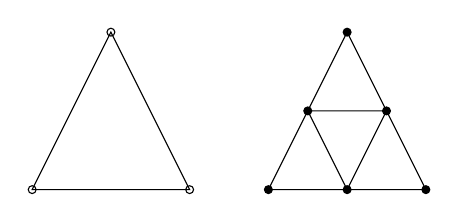
\begin{tikzpicture}
        % ������
        \draw (2, 1) -- (4, 1) -- (3, 3) -- cycle;
        % ��������
        \draw (2, 1) circle(0.05cm);
        \draw (4, 1) circle(0.05cm);
        \draw (3, 3) circle(0.05cm);
        % �ĸ�������
        \draw (5, 1) -- (6, 3) -- (7, 1) -- cycle;
        \draw (5.5, 2) -- (6.5, 2) -- (6, 1) -- cycle;
        % ��������
        \draw [fill = black] (5, 1) circle(0.05cm);
        \draw [fill = black] (6, 3) circle(0.05cm);
        \draw [fill = black] (7, 1) circle(0.05cm);
        \draw [fill = black] (5.5, 2) circle(0.05cm);
        \draw [fill = black] (6.5, 2) circle(0.05cm);
        \draw [fill = black] (6, 1) circle(0.05cm);
      \end{tikzpicture}
      \caption{��: ѹ�� ~$p$ ��Ԫ, $\circ$ Ϊ~$p$ ��Ԫ�ϵ����ɶ�;
               ��: 4���ٶ�~$v$ ��Ԫ, $\bullet$ ��ʾ~$v$ ��Ԫ�ϵ����ɶ�.}
      \label{fig::p-v-chap2}
    \end{figure}

\section{�����Ŵ����ṹ}
    ����һ���У������ᵽ�ٶȵ�Ԫ��ѹ����Ԫ֮�������������������Ľ���������~\cite{li2005multi}
    �еļ����Ŵ����ṹ���������ṹ��������~$h-$ ����Ӧ���������Ǿͽ���һ���������ṹ��

    ��~$h-$ ����Ӧ�У����������һ���������(����һ���ᵽ���ٶ�~$\vec{u}$ ��ѹ��~$p$)���п����ڲ�ͬ�ĵط��������죬
    �����Ҫ�ֱ���������������ɢ��ֵ�⡣��ƴװ~$\int_{\Omega} \nabla \cdot \vec{u} p$ ��һ��ʱ����Ϊ~$\vec{u}$
    ��~$p$ �ڲ�ͬ�������ϣ������Ҫ������������֮�����ϵ���������������ڼ���������˵����С�������������죬
    �õ�������Ҫ�����������ֵĵط�����dz����С��ر�أ������С������Ԫ����������Ԫ�������ϰٱ���
    ��ʱ������������֮���Ӧ�Ĵ����Ƿdz�����ġ�Ϊ�˴�����Ч�Ķ���������Ӧ���ԣ�\cite{li2005multi} ��ѡȡ
    �˼����Ŵ����������Ŵ��Ե�����ṹ��������Ϊ�㡢�ߡ��桢�塣��������޽ṹ���񣬼���Ҳ��ͨ������������ܵġ�
    ���ֲַ�����ݽṹ�����ṩ�򵥵ı�̷����Ϳ��ٵ���������㷨���Լ����������������

    �����Զ�ά����~$\Omega$ �ϵ�һ�������ʷ�~$\mathcal{T}_0$ Ϊ����������һ�¼����Ŵ����ṹ��Ϊ������Ԫ�ռ�ĵ�Ԫ
    ���ֿ����������ʷ��еĵ�ԪΪ���ε�Ԫ��$\tau$ Ϊ~$\mathcal{T}_0$ �ļ��ε�Ԫ�������ʷ������м������ʶ������ڵ�
    ��ϵ�������һ������һ�������������е�һ�������������������������Ρ�ͬ���ģ����һ������һ������������
    �е�һ���������������������ߡ������ʷ��е�һ�������ο��Ա����ܳ��ĸ�С�������Ρ��������μ��ܵĹ����У���
    ���߷ֱ𱻷ֳ��������֡��������ʷ������е������ζ�����һ�Σ����ǿ��Եõ�һ�����ܵ������ʷ�~$\mathcal{T}_1$��
    �����~$\mathcal{T}_0$ ��һ��ȫ�ּ��ܡ�������μ��ܣ����ǿ��Եõ�һϵ�е������ʷ�~$\{ \mathcal{T}_n\}$�� ���
    ~$\mathcal{T}_n$ �е�һ��������~$\tau_1$ λ��~$\mathcal{T}_{n-1}$ �е�������~$\tau_0$ �У���~$\tau_1$ ��������~$\tau_0$
    ��һ�����ӡ����Ǹ�~$\mathcal{T}_0$ �е�����������һ������ĸ��ף������д�~$\mathcal{T}_0$ ����������������������
    �IJ��������һ���������ݽṹ����ͼ~\ref{fig::hgeometrytree_chap2} ��ʾ�������Ҳ����Ϊ�����Ŵ�����
    \begin{figure}[h]
        \begin{minipage}[t]{0.4\textwidth}
          \centering
          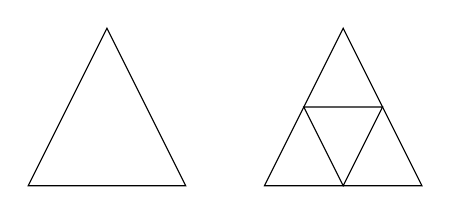
\begin{tikzpicture}
            % ������
            \draw (2, 1) -- (4, 1) -- (3, 3) -- cycle;
            \draw (5, 1) -- (6, 3) -- (7, 1) -- cycle;
            \draw (5.5, 2) -- (6.5, 2) -- (6, 1) -- cycle;
          \end{tikzpicture}
          \caption{ȫ�ּ���һ�ε�����}
        \end{minipage}
        \begin{minipage}[t]{0.6\textwidth}
          \centering
          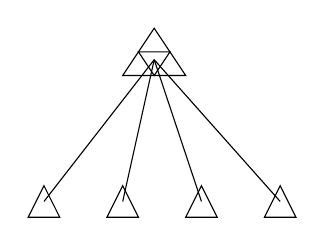
\begin{tikzpicture}
            %���������
            \draw (1.0, 0.0) -- (1.2, 0.4) -- (1.4, 0.0) -- cycle;
            \draw (2.0, 0.0) -- (2.2, 0.4) -- (2.4, 0.0) -- cycle;
            \draw (3.0, 0.0) -- (3.2, 0.4) -- (3.4, 0.0) -- cycle;
            \draw (4.0, 0.0) -- (4.2, 0.4) -- (4.4, 0.0) -- cycle;
            \draw (2.6, 2.4) -- (2.2, 1.8) -- (3.0, 1.8) -- cycle;
            \draw (2.4, 2.1) -- (2.6, 1.8) -- (2.8, 2.1) -- cycle;
            %������
            \draw (2.6, 2.0) -- (1.2, 0.2);
            \draw (2.6, 2.0) -- (2.2, 0.2);
            \draw (2.6, 2.0) -- (3.2, 0.2);
            \draw (2.6, 2.0) -- (4.2, 0.2);
          \end{tikzpicture}
          \caption{���ļ����Ŵ���}
        \end{minipage}
      \caption{�����Ŵ����ṹ}
      \label{fig::hgeometrytree_chap2}
    \end{figure}
    �ü����Ŵ����ṹ������h-����Ӧ�����ݾͲ�����ϸ�����ˡ�

\section{�ƶ����񷽷�}
    �ƶ����񷽷�����������ֵ�����У�Ѱ�Һõ�����(�����������й�)������
    �����Ͻ�����ֵ��⣬ʹ���ڲ��������ɶȵ�ǰ���£������ܵ���߼��㾫
    �ȡ��ƶ����񷽷�����������ƶ����ԣ��Լ��ڷ����������ϵ���ֵ�����
    ������~\cite{budd2009adaptivity}��\cite{huang2010book}��\cite{tang2007book}
    ��ϵͳ�ظ������ƶ����񷽷��Ľ��ܡ��ƶ�����IJ����ǻ��ڵȷֲ�ԭ��
    (Equi-distribute Principle)������~de Boor ��~$1974$ ��~\cite{boor1974goodII}
    ����ġ��ȷֲ�ԭ���Ǹ���һ���ܷ�ӳ�ֲ��������������ָ�꣬������
    �ƶ�����ڵ�ʹ�����ָ���������Ͼ��ȷֲ�������ڼ��������Ƚϴ��
    �ط������У�����ʹ�����ֲ��ıȽϾ��ȣ��Ӷ���߼��㾫�ȡ�

    ���Dz���֤���ظ���һά�����µĵȷֲ�ԭ�������£�
    \begin{theorem}
        ��һά�ռ��У�������һ������ ~$M = M(x) > 0, x \in [a, b]$������һ��������
        ~$N > 0$�������� ~$[a, b]$ �ʷֳ� ~$N$ �� ~$[x_0, x_1], \cdots [x_{N-1}, x_N]$��
        ʹ������Щ������
        \begin{equation}
            \int_{x_0}^{x_1}M(x)dx = \int_{x_1}^{x_2}M(x)dx = \cdots = \int_{x_{N-1}}^{x_{N}}M(x)dx,
        \end{equation}
        ��������ô�����ʷ��Ǵ���Ψһ�ġ�
    \end{theorem}
    ��� ���� ~$M(x)$ ȡ�������������Ǹ����ͬ�׵�������ô�����ʷ�ʹ�������ÿ��������
    ����ȡ�ͨ�����dz� ~$M$ Ϊ����Ŀ��ƺ���������~$\Omega, \Omega_c$ �ֱ�Ϊ��������ͼ�������
    ��ô ~$\Omega$ �� ~$\Omega_c$ ֮�������任�����õ���ӳ�������졣Dvinsky ~\cite{dvinsky1991adaptive} �� ~\cite{brackbill1993adaptive}
    ָ������ӳ�����Ӧ�õ�����Ӧ����������С�����ӳ��Ĵ���Ψһ���� ~\cite{hamilton2006harmonic} �� ~\cite{schoen1978univalent} �и�����
    ��� ~$\Omega_c$ ���������Ƿ����ģ����� ~$\partial \Omega_c$ �� ~$\Omega_c$ �µĶ�����͹�ģ���ô�� ~$\Omega$ �� ~$\Omega_c$
    �ĵ���ӳ����Ψһ�ġ������ ~$\Omega_c$ ѡΪ͹���򣬲����� ~$\Omega_c$ ����ŷʽ�����������������������������㡣
    ͨ����ⷽ��
    \begin{equation}
        \frac{\partial }{\partial x_i}\left( G^{ij}\frac{\partial \vec{\xi}}{\partial x_j}\right) = 0,
    \end{equation}
    ���Եõ��� ~$\Omega$ �� ~$\Omega_c$ �ĵ���ӳ�䡣���� ~$\vec{\xi}$ ���߼���������꣬~$x_i$ ��������������� ~$\vec{x}$ �ķ�����
    �� ~$M = 1/G^{ij}$ ��Ϊ���ƺ�����

    Li ��~\cite{li2001moving} �����һ���ƶ�����Ԫ���������ǻ��ڵ���ӳ�����۵ġ���Ҫ�뷨����ѡȡһ����ʼ���߼�
    ���򣬽�����ó�ʼ�������򵽳�ʼ�߼�����֮��ĵ���ӳ�䣬�����ⷢչ�У�ʹ����������Ķ�Ӧ���߼������𽥽�
    ���ڵ���ӳ�䡣ͨ�����һ��~Possion ����
    \begin{equation}
        \begin{aligned}
            \Delta \vec{\xi}  & = 0,& \\
            \vec{\xi}|_{\partial \Omega} &= \vec{\xi}_b,&
        \end{aligned}
        \label{eq::harmonic_map_eq}
    \end{equation}
    �����һ����ʼ���߼����� ~$\vec{\xi}^0$���൱�ڿ��ƺ���ȫ��ȡ ~$1$�������ʼ�߼�������֮���ں���ļ����б��ֲ��䡣
   \begin{algorithm}
     \caption{�������·ֲ�}
     \begin{algorithmic}[1]
        \State ������������ ~$\vec{x}^{(n)}$ �ϵ���ֵ��~$\vec{u}^{(n)}$
               ��ͨ����� ~\eqref{eq::harmonic_map_eq}�����~$\vec{\xi}^*$. \label{state::monitor_chap2}
        \State �ж�~$\parallel \vec{\xi}^* - \vec{\xi}^{(0)} \parallel_{L^2}$ �Ƿ�С��������
               ~$\epsilon$�� ����ǵ������������򣬼�����
               ~\ref{state::start_chap2} - \ref{state::end_chap2}��
        \State ��~$\vec{\xi}^* - \vec{\xi}^{(0)}$ ����֮��������
               ����������ƶ���~$\delta \vec{x}$��
               \label{state::start_chap2}
        \State ����~\ref{state::start_chap2}��~$\delta \vec{x}$, ������
               ~$\vec{x}^{(n)}$ �Ͻ� ~$\vec{u}^{(n)}$ ���µ���������
        \State �������� ~$\vec{x}^{(n)} \gets \vec{x}^{(n)} + \eta \delta \vec{x}$
        \State �ص�~\ref{state::monitor_chap2}. \label{state::end_chap2}
        \State ��������� ~$\vec{x}^{(n + 1)} = \vec{x}^{(n)}$�� �Լ������ϵ���ֵ�� ~$\vec{u}^{(n)}$
     \end{algorithmic}
     \label{alg::solve_mesh}
   \end{algorithm}
   �ڽ��������ϵ���ֵ���ֵ���������ϵĹ����У�Li \cite{li2001mesh} �����һ�ֱ�����ֵ�� ~$L_2$ ������ͬ�׷�����
   Di \cite{di2008general} �� Wang \cite{Wang2008} Ӧ�ô����������񷽷����� ~\eqref{eq::harmonic_map_eq} �����
   ����Ҫָ�����������ƶ�����Ԫ������������ƶ����������̵����ֱ������Ӷ�ʹ�ó���д�����dz����㡣��Բ�ͬ
   ���������⣬ֻҪ�ṩ���ʵĿ��ƺ������Լ������������ֵ��IJ��ֳ��򼴿ɡ�������㷨 ~\ref{alg::solve_mesh} ��
   ����д��������Ӧ����Ԫ������~AFEPack(\cite{AFEPack}) �С�
 \section{Ԥ��������}
    ���ǽ��ֱ��~Stokes ���̺�~Navier-Stokes ���̣�����Ԥ�����ķ��������������ȸ������Ԥ������~MINRES ������
    ~MINRES ������~Krylov �ӿռ䷽�������ԳƲ���ϵͳ�ġ����ǿ��������
    \begin{equation}
        M^{-1} K \vec{x} = M^{-1} \vec{b},
    \end{equation}
    ������ ~$K \vec{x} = \vec{b}$������ ~$K$ �ǶԳƲ�������~$M$ ��Ϊ ~$K$ ��Ԥ��������Ϊ�˱��־���Գ����ʣ�
    ~$M$ �ǶԳ���������ͨ�� ~$M$ ��ѡȡҪ��֤���㣬һ�����ܺܺõؽ��ƾ��� ~$A$��һ��Ҫ��� ~$M^{-1}$ Ҫ���ס�
    ��ʼ�в� ~$\vec{r}^{(0)} = \vec{b} - K\vec{x}^{(0)}$��$k$ �ε��� ~$\vec{x}^{(k)}$ ����
    ���� ~$M^{-1}K$ �� ~$M^{-1}\vec{r}^{(0)}$ �ųɵ�Krylov�ӿռ�
    \begin{equation}
        \vec{x}^{(0)} + \mathcal{K}_k(M^{-1}, M^{-1}\vec{r}^{(0)}),
    \end{equation}
    ���� ~$k$ �����������
    \begin{equation}
        \vec{z}^{(k)} \in M^{-1}\vec{r}^{(0)} + \mathcal{K}_k(M^{-1}K, M^{-1}\vec{r}^{(0)}),
    \end{equation}
    ����
    \begin{equation}
        \mathcal{K}_k(A, \vec{x}) := \mbox{span}\{\vec{x}, A\vec{x}, A^2\vec{x}, \cdots, A^{k - 1}\vec{x}\}.
    \end{equation}
    ���Ǹ���Ԥ������~MINRES �����㷨��
    \begin{algorithm}
%        \floatname{algorithm}
        \caption{Ԥ������~MINRES ����}
        \begin{algorithmic}[1]
        \State $\vec{v}^{(0)} = \vec{0}, \vec{w}^{(0)} = \vec{0}, \vec{w}^{(1)} = \vec{0}, \gamma = 0$
        \State ѡȡ ~$\vec{u}^{(0)}$������ ~$\vec{(1)} = \vec{b} - K\vec{x}$
        \State ��� ~$M\vec{z}^{(1)} = \vec{v}^{(1)}$���� ~$\gamma_1= \sqrt{<\vec{z}^{(1), \vec{z}^{(1)}}>}$
        \State �� ~$\eta = \gamma_1, s_0 = s_1 = 0, c_0 = c_1 = 1$
        \For {$j = 1 \to$ �в�С��������}
            \State $\vec{z}^{(j)} = \vec{z}^{(j)} / \gamma_j$
            \State $\delta_j = <K\vec{z}^{(j)}, \vec{z}^{(j)}>$
            \State $\vec{v}^{(j + 1)} = K \vec{z}^{(j)} - (\delta_j/\gamma_j)\vec{v}^{(j)} - (\gamma_j/\gamma_{j - 1})\vec{v}^{(j - 1)}$
            \State ��� ~$M\vec{z}^{(j + 1)} = \vec{v}^{(j + 1)}$
            \State $\gamma_{j + 1} = \sqrt{<\vec{z}^{(j + 1)}, \vec{z}^{(j + 1)}>}$
            \State $\alpha_0 = c_j\delta_j - c_{j - 1}s_j\gamma_j$
            \State $\alpha_1 = \sqrt{\alpha_0^2 + s\gamma_{j + 1}^2}$
            \State $\alpha_2 = s_j\delta_j + c_{j - 1}c_j\gamma_j$
            \State $\alpha_3 = s_{j - 1} \gamma_j$
            \State $c_{j + 1} = \alpha_0/\alpha_1; s_{j + 1} = \gamma_{j + 1}/\alpha_1$
            \State $\vec{w}^{(j + 1)} = (\vec{z}^{(j)} - \alpha_3 \vec{w}^{(j)})/\alpha_1$
            \State $\vec{u}^{(j)} = \vec{u}^{(j - 1)} + c_{j + 1}\eta\vec{w}^{j + 1}$
            \State $\eta = -s_{j + 1}\eta$
            \State ����в�
       \EndFor
    \end{algorithmic}
    \label{alg::precond_minres}
    \end{algorithm}
    ���㷨 ~\ref{alg::precond_minres} �У�Ԥ�����IJ���������� ~$M \vec{z}^{(j + 1)} = \vec{v}^{(j + 1)}$��
    �����ǵ�ʵ�ʼ����У�������Ҫͨ��ʵ�� ~$M^{-1}$ ��������ﵽԤ�����Ĺ��̡�����Ĺ���~Krylov �ӿռ��֪ʶ
    ���Բο� ~\cite{saad2003iterative}��\cite{van2003iterative}�ȡ�ͬ���أ������ǶԳƵIJ��������ʱ����
    ~Navier-Stokes ������ɢ����~Ossen ���⣬��ʱ������Ҫ��~GMRES(general minimal residual) ����⣬���ǹ�ע����
    Ԥ�������֣������㷨���ٸ�������� ~\cite{saad1986gmres}��

    \subsection{���Stokes����}
        ����ͨ��ѡȡ����Ԫ�ռ��������~\eqref{eq::weak_form_stokes_momentum} �� ~\eqref{eq::weak_form_stokes_mass}
        ������ɢ�����Եõ�һ�����Է����⣬���Ƕ���������Է������
        ϵ������Ϊ��
        \begin{equation}
            K = \left[
                \begin{array}{ll}
                 \vec{A} & B^T\\
                 B & -C
                \end{array}
                \right],
            \label{eq::coffient_stokes}
        \end{equation}
        �������������~LBB �����Ļ��Ԫ�����ƣ��� ~$C = 0$����Ϊ����������ѡȡ��������~LBB ������~$4P_1-P_1$ Ԫ������������������� ~$C = 0$ �����Ρ��� ~$\vec{v}_h \in X_h$ �� ~$q_h \in P_h$��$X_h$ �� ~$P_h$
        ���ڵ�һ�����ᵽ������Ԫ�ռ䡣������������ ~$\vec{v}_h, q_h$ �ķ�����
        \begin{align}
            ||\nabla \vec{v}_h|| := <\vec{A}\vec{v}, \vec{v}>^{1/2}, \\
            ||q_h|| := <Qq, q>^{1/2},
            \label{eq::norm}
        \end{align}
        ����~$\vec{v}$ �� ~$\vec{q}$ ���ٶȺ�ѹ�������ڻ�����~$\{\vec{\phi}_j \}_{j = 1}^{n_u}$ �� ~$\{\vec{\psi}_k \}_{k = 1}^{n_p}$ �µ�ϵ��������� ~$\vec{A}$ ����ɢ��������ʽ�ĸնȾ���
        \begin{eqnarray}
            \vec{A} = [a_{ij}], \quad a_ij = \int_\Omega \nabla \vec{\phi}_i : \nabla \vec{\phi}_j, \qquad i,j = 1, \cdots, n_u,
        \end{eqnarray}
        ���� ~$Q$ ��ѹ����������
        \begin{equation}
            Q = [q_{kl}],\quad q_{kl} = \int_\Omega \psi_k \psi_l, \qquad k,l = 1, \cdots, n_p.
        \end{equation}
        �����ñ�׼�ķ�����ʽ���������������ڶ�ά����������
        \begin{equation}
            <\vec{A}\vec{v}, \vec{v}> \equiv <A\vec{v}_x, \vec{v}_x> + <A\vec{v}_y, \vec{v}_y>,
        \end{equation}
        ���� ~$A$ �� ~$n \times n$ ��������˹����
        ���� ~$B \vec{A}^{-1} B^T$ Ϊѹ��~Schur ���������ǿ���~$Q^{-1}B\vec{A}^{-1}B^T$ ������ֵ�ķ�Χ�������ȿ��DZ߽�ȫ����~Dirichlet �߽���������⣬�����ȸ���һЩ���塣
        \begin{definition}
            \label{def::min_angle_cond}����һϵ�е���������~$\{\mathcal{T}_h\}$���������һ����С�ĽǶ�
            ~$\theta_* > 0$��ʹ��~$\mathcal{T}_h$�е����е�Ԫ����~$\theta_{T} > \theta_*$����ô~$\mathcal{T}_h$ ������������ġ�
        \end{definition}
        \begin{proposition}
            \label{pro::bound_mass} ����~$\mathbb{R}^2$ �ռ��еľ������������ʵ�һ���ʷ֣�$\vec{P}_1$ �ǽ���������ʷ��ϵ�һ�����ƣ���ô��������~$Q$ �����µ���ʽ����
            ���������:
            \begin{equation}
                c\uline{h}^2 \leq \frac{<Q\vec{v}, \vec{v}>}{<\vec{v}, \vec{v}>} \leq Ch^2,
                \label{eq::bound_mass}
            \end{equation}
            �����е�~$\vec{v} \in \mathbb{R}^n$������~$\uline{h} = \min_{\bigtriangleup_k \in \mathcal{T}_h} h_k$
            ���� ~$h = \max_{\bigtriangleup_k \in \mathcal{T}_h} h_k$������~$c$ �� ~$C$ ���Ǹ�~$\uline{h}$ �� ~$h$ �޹صġ�
        \end{proposition}

        \begin{definition}[��һ���ʷ�]
            \label{theo_quasi_uni_subd}����һϵ�е���������~$\{\mathcal{T}_h\}$�����������һ������~$\rho > 0$ ʹ�ö���
            ~$\{\mathcal{T}_h\}$ �е�ÿһ�����񣬶��� ~$\uline{h} \geq \rho h$����ô���Ǿͳ� ~$\{\mathcal{T}_h\}$  ����һ�µġ�
        \end{definition}

        ����~$\mathcal{R}^2$ �ռ��һ����һ���ʷ֣��������ĵ�Ԫ����������ģ���ô���� ~\eqref{eq::bound_mass} ���Լ�Ϊ:
        \begin{equation}
            c h^2 \leq \frac{<Q \vec{v}, \vec{v}>}{<\vec{v}, \vec{v}>} \leq C h^2, \quad \mbox{�����е�} \vec{v} \in \mathbb{R}^n.
            \label{eq::bound_mass_simpify}
        \end{equation}
        \eqref{eq::bound_mass_simpify} �Ǹ��ռ��ά���йصġ����� ~$\mathbb{R}^3$ �е�һ�����򣬽�����һ���ʷ֣�������ʷ���
        �����������嵥Ԫ����Ӧ�н磺
        \begin{equation}
            c h^3 \leq \frac{<Q \vec{v}, \vec{v}>}{<\vec{v}, \vec{v}>} \leq C h^3, \quad \mbox{�����е�} \vec{v} \in \mathbb{R}^n.
            \label{eq::bound_mass_R3}
        \end{equation}

        \begin{remark}
            ����ʷ�����һ�µģ���ô�����������~$\vec{P}_m, m \geq 2$���н��� ~\eqref{eq::bound_mass_simpify} ��������
            ���� ~$c$ �� ~$C$ ���� ~$m$ �йء�
        \end{remark}

        \begin{theorem}
            \label{theo::mass_spectrual_eq} ���� ~$\partial \Omega = \partial \Omega_D$ ���������⣬������ LBB �����Ļ��Ԫ��
            �Ʋ��� ~$\mathbb{R}^2$ �ϵ���һ���ʷ���������ģ���
            ѹ��Schur������~$B \vec{A}^{-1} B^T$ �׵ȼ���ѹ����������~$Q$:
            \begin{equation}
                \gamma^2 \leq \frac{<B \vec{A}^{-1} B^T \vec{q}, \vec{q}>}{<Q\vec{q},\vec{q}>} \leq 1 \quad \mbox{�����е�}
                \vec{q} \in \mathbb{R}^{n_p} \mbox{ʹ��} \vec{q} \neq \vec{1}.
                \label{eq::lower_uper_bound}
            \end{equation}
            inf-sup ����~$\gamma$ �� ~$0$�����Ҹ�����߶�~$h$ �޹ء�����ѹ�� ~Schur �����������������
            \begin{equation}
                \kappa(B\vec{A}^{-1}B^T) \leq C/(c\gamma^2),
            \end{equation}
            ����~$c$ �� ~$C$ ��~\eqref{eq::bound_mass_simpify} �еij�����
        \end{theorem}

        \begin{proof}
            ��������֤���½硣��ɢ~inf-sup �ȶ��������Ĵ�����ʾ��
            \begin{equation}
                \gamma \leq \min_{q_h \neq \mbox{constant}} \max_{\vec{v}_h \neq \vec{0}} \frac{|(q_h, \nabla \cdot \vec{v}_h)|}{||\nabla \vec{v}_h|| ||q_h||}.
            \end{equation}
            �ر�ģ�����~\eqref{eq::norm} �еľ�������������~$|(q_h, \nabla \cdot \vec{v}_h)| = (\vec{q}, B\vec{v})$, �����У�
            \begin{align}
                \gamma & \leq \min_{\vec{q} \neq \vec{1}} \max_{\vec{v} \neq \vec{0}} \frac{|<\vec{q}, B\vec{v}>|}{<\vec{A}\vec{v}, \vec{v}>^{1/2} <Q\vec{q}, \vec{q}>^{1/2}} &\\ \notag
                & = \min_{\vec{q} \neq \vec{1}} \frac{1}{<Q\vec{q}, \vec{q}>^{1/2}} \max_{\vec{w} = \vec{A}^{1/2}\vec{v} \neq \vec{0}} \frac{|<\vec{q}, B \vec{A}^{-1/2} \vec{w}>|}{<\vec{w}, \vec{w}>^{1/2}} &\\ \notag
                & = \min_{\vec{q} \neq \vec{1}} \frac{1}{<Q\vec{q}, \vec{q}>^{1/2}} \max_{\vec{w} \neq \vec{0}} \frac{|<\vec{A}^{-1/2}B^Tq, \vec{w}>|}{<\vec{w}, \vec{w}>^{1/2}} &\\ \notag
                & = \min_{\vec{q} \neq \vec{1}} \frac{<\vec{A}^{-1/2}B^Tq, \vec{A}^{-1/2}B^Tq>^{1/2}}{<Q\vec{q}, \vec{q}>^{1/2}} &\\ \notag
                & = \min_{\vec{q} \neq \vec{1}} \frac{<B \vec{A}^{-1}B^T\vec{q}, \vec{q}>^{1/2}}{<Q\vec{q}, \vec{q}>^{1/2}}.& \notag
            \end{align}
            ��Ϊ���ļ���ֵ��~$\vec{w} = \pm \vec{A}^{-1/2}B^T \vec{q}$ ʱȡ������ˣ����ǿ��Կ���
            \begin{equation}
                \gamma^2 = \min_{\vec{q} \neq \vec{1}} \frac{<B\vec{A}^{-1}B^T \vec{q}, \vec{q}>}{<Q\vec{q}, \vec{q}>},
                \label{eq::lower_bound}
            \end{equation}
            ���½��֤��
            ����������֤���Ͻ磬�Ͻ�����΢�����ӵ����ʵõ��ġ����ȣ�Ӧ��~Cauchy-Schwarz ����ʽ��������
            \begin{equation}
                |(q_h, \nabla \cdot \vec{v}_h)| \leq ||q_h|| ||\nabla \cdot \vec{v}_h||.
                \label{eq::cauchy_schwarz_inequality}
            \end{equation}
            �ڶ���ע�⵽ ~$\vec{v}_h \in \mathcal{H}_0^1$(��Ϊ~$\partial \Omega = \partial \Omega_D$)���� ~$\vec{v}_h$ ���뵽���е�ʽ�У�
            \begin{equation}
                \int_{\Omega} \nabla \vec{w} : \vec{v} \equiv \int_{\Omega} (\nabla \cdot \vec{w})(\nabla \cdot \vec{v}) + \int_{\Omega} (\nabla \times \vec{w}) : (\nabla \times \vec{v}),
            \end{equation}
            ���������ʽ�Ƕ���������~Soblev �ռ�
            \begin{equation}
                \mathcal{H}_0^1 = \{ \vec{u} \in \mathcal{H}^1(\Omega) | \vec{u} = \vec{0} \mbox{��} \partial \Omega \mbox{��} \},
            \end{equation}
            �е����⺯��~$\vec{w}, \vec{v}$ �������ģ����������
            \begin{equation}
                ||\nabla \vec{v}_h||^2 = ||\nabla \cdot \vec{v}_h||^2 + ||\nabla \times \vec{v}_h||^2 \geq ||\nabla \cdot \vec{v}_h||^2.
                \label{eq::identiy_v_h}
            \end{equation}
            ��󣬽�� ~\eqref{eq::cauchy_schwarz_inequality} �� ~\eqref{eq::identiy_v_h}�����ǵõ�
            \begin{equation}
                \frac{|(q_h, \nabla \cdot \vec{v}_h)|}{||\nabla \vec{v}_h|| ||q_h||} \leq 1.
            \end{equation}
            ����ʽչ���ɾ�����ʽ�����Ƶ� ~\eqref{eq::lower_bound} �����ƣ����Եõ� ~\eqref{eq::lower_uper_bound} �е��Ͻ硣
            ���� ~\eqref{eq::bound_mass_simpify} �е������������������н��ԣ����ǿ��Եõ� ~Schur ��������������н�
            \begin{equation}
                \gamma^2 \frac{<Q\vec{q}, \vec{q}>}{<\vec{q}, \vec{q}>} \leq \frac{<B \vec{A}^{-1}B^T \vec{q}, \vec{q}>}
                {<\vec{q}, \vec{q}>} \leq \frac{<Q \vec{q}, \vec{q}>}{<\vec{q}, \vec{q}>}.
            \end{equation}
        \end{proof}

        \begin{remark}
            �� ~$\mathbb{R}^3$ �е���һ���ʷ��ϵ������嵥Ԫ��������ȶ��Ļ��Ԫ���ƣ���ô~Schur
            ��������н���ͬ������������������н����� ~\eqref{eq::bound_mass_R3} �и�����
        \end{remark}

        ͬ���أ����ڱ߽��а��� ~Neumann �������������⣬����ֵ�Ľ������� ~\ref{pro::schur_bound_neumann} �и�����

        \begin{proposition}
            \label{pro::schur_bound_neumann}������ ~$\int_{\partial \Omega_N} ds \neq 0$ ���������⣬��һ��һ���ȶ��Ļ��Ԫ����ȥ��ɢ��
            ����������Ԫ�����ǽ����� ~$\mathbb{R}^d$ �ϵ�һ����������һ�µ��ʷ��ϣ���ôѹ��~Schur ����������
            \begin{equation}
                \gamma_N^2 \leq \frac{<B\vec{A}^{-1}B^T \vec{q}, \vec{q}>}{<Q\vec{q}, \vec{q}>} \leq \Gamma^2, \quad \mbox{�����е� } \vec{q} \in \mathbb{R}^{n_p}.
                \label{eq::schur_bound_neumann}
            \end{equation}
            ���г��� ~$\gamma_N$ �Dz�Ϊ~$0$ ���н糣�������Ҹ�����߶� ~$h$ �޹أ�$\Gamma < \sqrt{d}$ $d$ �ǿռ�ά����
        \end{proposition}
        ���� ~$P_2-P_1, Q_2-Q_1$ ���Ԫ���ƣ�������~inf-sup �����ģ�������һ����Ϊ ~$0$ ��~inf-sup ���� ~$\delta$��ʹ��
        \begin{equation}
            \delta \leq \min_{q_h \neq \mbox{constant}} \max_{\vec{v}_h \neq \vec{0}} \frac{|(q_h, \nabla \cdot \vec{v}_h)|}{||\vec{v}_h|| ||\nabla q_h||}.
            \label{eq::inf_sup_p2p1}
        \end{equation}
        �������� ~$L^2(\Omega)$ �ռ��й����ٶȣ��� ~$\mathcal{H}^1(\Omega)$ �й���ѹ�������һ���~inf-sup ������Щ�෴���������������ٶ��������� ~$\heiti{Q}$��
        \begin{equation}
            \heiti{Q} = [\heiti{q}_{ij}], \quad \heiti{q}_{ij} = \int_{\Omega} \vec{\phi}_i \cdot \vec{\phi}_j, \qquad i,j = 1, \cdots, n_u,
        \end{equation}
        ��ѹ���ĸնȾ��� ~$A_p$��
        \begin{equation}
            A_p = [a_{kl}], \quad a_{jl} = \int_{\Omega} \nabla \psi_k \cdot \psi_l, \qquad i,j = 1, \cdots, n_p.
        \end{equation}
        ��ô���� ~\eqref{eq::lower_bound} ���Ƶ����� ~\eqref{eq::inf_sup_p2p1} ��������дΪ
        \begin{equation}
            \delta^2 = \min_{\vec{q} \neq \vec{1}} \frac{<B \heiti{Q}^{-1} B^T \vec{q}, \vec{q}>}{<A_p\vec {q}, \vec{q}>}.
            \label{eq::spectral_equal_Ap_D}
        \end{equation}
        ����~$B \heiti{Q}^{-1} B^T$ ͨ��������һ��ѹ�����ɾ������ ~\cite{gresho1998incompressible}�����ڷ������ı߽��������������������ģ���������£���
        ������ġ����� ~$P_2-P_1$ ���Ƶ������С����ֵ�����Ƿ����ھ��������ϣ����ҶԷ������ı߽���������
        \begin{equation}
            \frac{1}{2} < \frac{<B \heiti{Q}^{-1} B^T \vec{q}, \vec{q}>}{<A_p \vec{q}, \vec{q}>} \leq 1, \quad \mbox{�����е� } \vec{q} \in \mathbb{R}^{n_p}, \vec{q} \neq \vec{1}.
            \label{eq::spectral_equal_Ap_N}
        \end{equation}

        ���ǿ��� ~\eqref{eq::coffient_stokes} �Ŀ�Խ�Ԥ��������
        \begin{equation}
            M = \left[
                \begin{array}{ll}
                 \vec{P} & 0\\
                 0 & T
                \end{array}
                \right],
            \label{eq::coffient_stokes_precond}
        \end{equation}
        ����~$\vec{P} \in \mathbb{R}^{n_u \times n_u}$ �� ~$T \in \mathbb{R}^{n_p \times n_p}$
        ���ǶԳ�������������Ҫ�� ~$\eqref{eq::coffient_stokes}$ ��һ���õĽ��ƣ���ζ������Ҫ��
        �����ʵ� ~$\vec{P}$ ���� ~$\vec{A}$ ���ҽ���~Schur �� ~$B \vec{A}^{-1} B^T$ �ľ��� ~$T$���Ӷ���
         ~\ref{theo::mass_spectrual_eq} ����֪����ѹ������������ ~$Q$ �ں��ʵı�
        �����������׵ȼ���~Schur ������ġ�������ǿ���ѡ�� ~$T = Q$���������� ~$\vec{P} = \vec{A}$��
        ���ǿ��ǹ��������ֵ����
        \begin{equation}
            \left[
            \begin{array}{ll}
                A & B^T \\
                B & 0 \\
            \end{array}
            \right]
            \left[
            \begin{array}{l}
                \vec{u} \\
                \vec{p} \\
            \end{array}
            \right] = \lambda
            \left[
            \begin{array}{ll}
                \vec{A} & 0 \\
                0 & Q \\
            \end{array}
            \right]
            \left[
                \begin{array}{l}
                    \vec{u} \\
                    \vec{p} \\
                \end{array}
            \right],
        \end{equation}
        ͨ���򵥵ļ������֪������ֵ ~$\lambda$ λ��
        \begin{equation}
            [ \frac{1 - \sqrt{1 + 4 \Gamma^2}}{2}, \frac{1 - \sqrt{1 + 4 \gamma^2}}{2} ] \cup \{1\} \cup [ \frac{1 + \sqrt{1 + 4 \gamma^2}}{2}, \frac{1 + \sqrt{1 + 4\Gamma^2}}{2}].
        \end{equation}
        ���� ~$\gamma$ �� ~$\Gamma$ �� ~\eqref{eq::lower_uper_bound} �� ~\eqref{eq::schur_bound_neumann} �е����½磬������߶� ~$h$ �޹صij�����
        ��ˣ����ǿ���֪���������Ԥ������~MINRES �����Ļ�����ܿ�����������������ɢ������߶�û�й�ϵ��

        �� ~\cite{elman2014finite} ��ָ�����ڲ�Ӱ��~MINRES ������ǰ���£����Կ����ñ� ~$T = \mbox{diag}(Q)$ ����Ϊ~Schur ������Ľ��ơ�
        �������� ~$T = Q$ �� ~$T = \mbox{diag}(Q)$ �����
        \begin{lemma}
            ����� ~$\mathbb{R}$ �ϵ�һ���ʷ��ϣ�ѹ���ռ��� ~$P_1$ Ԫ���ƣ�ѡȡ ~$T = \mbox{diag}(Q)$����ô
            ��
            \begin{equation}
                \theta^2 \leq \frac{<Q\vec{q}, \vec{q}>}{<T\vec{q}, \vec{q}>} \leq \Theta^2
                \quad \mbox{�����е� } \vec{q} \in \mathbb{R}^{n_p},
            \end{equation}
            ���������� ~$\theta = 1/\sqrt{2}$ �� ~$\Theta = \sqrt{2}$����������߶� ~$h$ �޹ء�
        \end{lemma}


        ���濼����θ��õĽ��� ~$\vec{A}$���������ȿ��Dz������������⣺
        �ҵ� ~$u \in \mathcal{H}_E^1$��ʹ��
        \begin{equation}
            a(u, v) = l(v) \mbox{�����е�} v \in \mathcal{H}_{E_0}^1.
            \label{eq::var_possion}
        \end{equation}
        \begin{proposition}[$\mathcal{H}$ ������]
            �������һ������ ~$C_{\Omega}$ ʹ�ö������ ~$f \in L_2(\Omega)$��������һ����
            ~$u \in \mathcal{H}_E^1 \subset \mathcal{H}^2(\Omega)$����������
            \begin{equation}
                ||u||_{\mathcal{H}^2} \leq C_{\Omega} ||f||,
            \end{equation}
            ��ô��Ʊ������ ~\eqref{eq::var_possion} �� ~$\mathcal{H}^2$ ����ġ�
        \end{proposition}

        \begin{theorem}
            ����һ�� ~$\mathcal{H}^2$ �������һ�� ~$\mathcal{R}^2$ �� ~$\mathcal{R}^3$ ������߶�
            Ϊ ~$h$ ����һ���ʷ֣�������һ�� ~$l$ ���������Wѭ������� ~$A\vec{u} = \vec{f}$����ô
            ����һ����С�Ĺ⻬���� ~$k_*$������ ~$h$ �޹أ����Ҵ���һ���н�IJ�Ϊ ~$1$ ��ѹ������ ~$\eta_l$��
            Ҳ���� ~$h$ �޹صģ���ô������
            \begin{equation}
                ||\vec{u} - \vec{u}^{(i + 1)}||_A \leq \eta_l ||\vec{u} - \vec{u}^{(i)}||_A.
            \end{equation}
            ���� ~$\vec{u}^{(i)}$ �� ~$l$ ���������������� ~$i$ ��ѭ���õ��ġ�
            \label{theo::multigrid_W}
        \end{theorem}
        ���� ~\ref{theo::multigrid_W} ��֤���� ~\cite{elman2014finite}��
        \begin{theorem}
            ����һ�� ~$\mathcal{H}^2$ ����������һ�� ~$\mathcal{R}^2$ �� ~$\mathcal{R}^3$ ������߶�
            Ϊ ~$h$ ����һ���ʷ֣�������һ���ԳƵ� ~$l$ ���������Vѭ������� ~$A\vec{u} = \vec{f}$����ô
            ��� ~$l$ �������������������ſ˱ȹ⻬�ӣ������һ��ѹ������ ~$\eta_l < 1$ ʹ��
            \begin{equation}
                ||\vec{u} - \vec{u}^{(i + 1)}||_A \leq \rho_l ||\vec{u} - \vec{u}^{(i)}||_A, \quad \rho_l \leq \rho_{\infty} := C/(C + k),
            \end{equation}
            ���� ~$C$ ��һ���� ~$l$ �޹صij���������~$k = m$ �ǹ⻬������
            \label{theo::multigrid_V}
        \end{theorem}
        ���� ~\ref{theo::multigrid_V} ��֤�����Բο�(\cite{braess1983new}��\cite{brenner2007mathematical})��

        \begin{lemma}
            ���������ϵͳ ~$\vec{A}\vec{u} = \vec{f}$ �У����������
            \begin{equation}
                \vec{u}^{(i + 1)} = (\vec{I} - \vec{P}^{-1}\vec{A}) \vec{u}^{i} + \vec{P}^{-1} \vec{f}
            \end{equation}
            �ĵ����������
            \begin{equation}
                ||\vec{u} - \vec{u}^{(i + 1)}||_A \leq \rho ||\vec{u} - \vec{u}^{(i)}||_A,
                \label{eq::iteration_error}
            \end{equation}
            ����ѹ������ ~$\rho < 1$�� ��ô
            \begin{equation}
                1 - \rho \leq \frac{<\vec{A}\vec{v}, \vec{v}>}{<\vec{P}\vec{v}, \vec{v}>} \leq
                1 + \rho \quad \mbox{�����е� } \vec{v}.
            \end{equation}
            \label{lemma::bound_P_A}
        \end{lemma}
        \begin{proof}
            ��Ϊ��ȷ�� ~$\vec{u}$ ����
            \begin{equation}
                \vec{u} = (\vec{I} - \vec{P}^{-1}\vec{A})\vec{u} + \vec{P}^{-1} \vec{f}, \notag
            \end{equation}
            \eqref{eq::iteration_error} ���Ա���Ϊ
            \begin{equation*}
                <\vec{A}(\vec{I} - \vec{P}^{-1}\vec{A})\vec{e}, (\vec{I} - \vec{P}^{-1}\vec{A})\vec{e}> \quad \leq \quad \rho^2 <\vec{A}\vec{e}, \vec{e}>,
            \end{equation*}
            ������� ~$\vec{e} = \vec{u} - \vec{u}^{(i)}$���� ~$\vec{v} = \vec{A}^{1/2}\vec{e}$, ��ô��ʽ��������д��
            \begin{equation*}
                <(\vec{I} - \vec{A}^{1/2}\vec{P}^{-1} \vec{A}^{1/2})\vec{v}, (\vec{I} - \vec{A}^{1/2}\vec{P}^{-1} \vec{A}^{1/2})\vec{v}> \leq \rho^2 <\vec{v}, \vec{v}>,
            \end{equation*}
            �����е� ~$\vec{v}$�����
            \begin{equation}
                -\rho <\vec{v}, \vec{v}> \leq <(\vec{I} - \vec{A}^{1/2}\vec{P}^{-1} \vec{A}^{1/2})\vec{v}, \vec{v})> \leq \rho <\vec{v}, \vec{v}>, \notag
            \end{equation}
            �����ǿ��Եõ�
            \begin{equation}
                1 - \rho \leq \frac{<\vec{A}\vec{v}, \vec{v}>}{<\vec{P}\vec{v}, \vec{v}>} \leq
                1 + \rho,
            \end{equation}
            �����е� ~$\vec{v}$��
        \end{proof}
        ��� ���� ~\ref{theo::multigrid_V}������ ~\ref{theo::multigrid_W} �� ����~\ref{lemma::bound_P_A}��
        ����ѡȡ���ʵ�ѹ���������ӣ���һ����������ѭ�������� ~$\vec{P}$�������Ԥ����������ѡ�� ~$\vec{P} = \vec{A}$��
        ������һ�ζ�������~$V$ �ͻ�~$W$ ��ѭ������~$P$����Ȼ~MINRES �����������������һЩ���������� ~$h$ �޹صġ��������
        �öԽǿ�ֱ����Ԥ��������MINRES �ĵ������������� ~$h$ �ļ�С�����ӡ�

    \subsection{���Navier-Stokes����}
        ���ȶ��Ļ��Ԫ����~Navier-Stokes ���̣���õ���~Stokes ���������Ƶ�����ϵͳ�����ǿ�������ϵ������
        \begin{equation}
            \left[
            \begin{array}{ll}
                \vec{F} & B^T \\
                B & 0 \\
            \end{array}
            \right],
        \end{equation}
        ���� ~$F$ ������������󣬲��ǶԳƵġ����ǿ�����~Krylov �ӿռ䷽���е�~GMRES ���������ϵͳ���ڱ����У�����
        ������~Ossen ϵͳ����
        \begin{equation}
            \left[
            \begin{array}{ll}
                \nu \vec{A} + \vec{N} & B^T \\
                B & 0 \\
            \end{array}
            \right]
            \left[
            \begin{array}{l}
            \vec{u} \\
            \vec{p} \\
            \end{array}
            \right] =
            \left[
            \begin{array}{l}
            \vec{f} \\
            \vec{0} \\
            \end{array}
            \right],
            \label{eq::ossen_system}
        \end{equation}
        ���� ~$\vec{A}$ ���ٶȿռ��������ʽ�ĸնȾ����Լ� ~$\vec{N}$ ��������ʽ�Ķ������󣬷ֱ������£�
        \begin{eqnarray}
            \vec{A} = [\vec{a}_{ij}], \quad \vec{a}_{ij} = \int_{\Omega}\nabla \vec{\phi}_i \cdot \vec{\phi}_j, \\
            \vec{N} = [\vec{n}_{ij}], \quad \vec{n}_{ij} = \int_{\Omega}(\vec{u}_h \cdot \vec{\phi}_i) \cdot \vec{\phi}_j.
        \end{eqnarray}
        Elman �� ~\cite{elman2014finite} ��ָ��������� ~\eqref{eq::ossen_system} ʱ���� �����Ǿ�����Ԥ�����ȿ�ԽǾ�����Ԥ������������������룬���(\cite{fischer1998minimum}��\cite{elman1996fast})��
        ����ѡ���ÿ����Ǿ���
        \begin{equation}
            M = \left[
                \begin{array}{ll}
                    \vec{M}_{\vec{F}} & B^T \\
                    0 & -M_S \\
                \end{array}
                \right],
            \label{eq::block_triangular_precond}
        \end{equation}
        ��ΪԤ����������Խǿ�Ԥ����������ȣ�ֻ�����˾��� ~$B^T$ �������˻�����������
        �����ȼ��� ~$\vec{M}_F = \vec{F}$��������һ��������⣬�����ô�������������⡣
        ���������������ݿ��Բο�����(\cite{brezina2005adaptive}��\cite{ruge1987algebraic})��
        ���������������ҵ� ~Schur ��Ԥ�������� ~$M_S$ ��Ч��ѡ��
        \begin{remark}
            ���ǿ�������~Stokes ���̣���ѹ������������ ~$Q$ ��Ϊ~Schur ��Ԥ����������(\cite{elman1996fast}��\cite{klawonn1999block}) �У�
            ָ������ŵ�� ~$Re < 10$ ������������������Ǹ������޹صģ���������~Reynolds ������
            �����ʻ�񻯡�
        \end{remark}
        �������ǿ������ֽ���~Schur ������ ~$B\vec{F}^{-1}B^T$ �ķ�����ѹ��������ɢԤ����(PCD precoditon) ����С���˽�����Ԥ����(LSC precondition)��
        �����������ٶȿռ��ѹ���ռ�Ķ�����ɢ����
        \begin{eqnarray*}
            \mathcal{L} & = & -\nu \nabla^2 + \vec{w}_h \cdot \nabla, \\
            \mathcal{L}_p &= & -(\nu \nabla^2 + \vec{w}_h \cdot \nabla)_p.
        \end{eqnarray*}
        ���ǿ��Ƕ�����ɢ���Ӻ�ɢ�����ӵĽ����ӣ�
        \begin{equation}
            \mathcal{E} = \nabla \cdot (-\nu \nabla^2 + \vec{w}_h \cdot \nabla) -
            (\nu \nabla^2 + \vec{w}_h \cdot \nabla)_p \nabla \cdot,
            \label{eq::commutor}
        \end{equation}
        �����������ij���������DZȽ�С�ġ�����������ѹ��������ɢԤ����(PCD precondition)��
        �� ~$Q^{-1}B$ �Ǹ���ɢ�����ӵľ��������ʽ��$\vec{Q}^{-1}B^T$ ����ɢ�ݶ����ӵ�
        ���������ʽ���� ~\eqref{eq::commutor} ����д����ɢ������ʽ
        \begin{equation}
            \mathcal{E}_h = (Q^{-1}B)(\vec{Q}^{-1}\vec{F}) - (Q^{-1}F_p)(Q^{-1}B),
            \label{eq::commutor_discrete}
        \end{equation}
        ���� ~$\vec{Q}$ ���ٶ���������$\vec{F}$ �� ~$F_p$ �ֱ����ٶȺ�ѹ���ռ�Ķ�����ɢ����
        ~$F_p$ ��
        \begin{equation}
            F_p = [f_{p,ij}], f_{p,ij} = \nu \int_{\Omega} \nabla \psi_j \cdot \nabla \psi_i + \int_{\Omega} (\vec{w}_h \cdot \nabla \psi_j) \psi_i.
        \end{equation}
        �� ~\eqref{eq::commutor_discrete} ���߳��� ~$\vec{F}^{-1}B^T$�����ǿ��Եõ�
        ~Schur �������һ�����ƣ�
        \begin{equation}
            B\vec{F}^{-1}B^T \approx QF_p^{-1}B\vec{Q}^{-1}B^T.
        \end{equation}
        �� ~\eqref{eq::spectral_equal_Ap_D} �� ~\eqref{eq::spectral_equal_Ap_N} �����ǵ�֪��
        ~$B\vec{Q}^{-1}B^T$ �Ǹ�ѹ���ռ�ĸնȾ������׵ȼ۵ġ�������ǿ��Եõ�ѹ��������ɢ
        Ԥ�������� ~\eqref{eq::block_triangular_precond} �е� ~$M_S$ ȡΪ
        \begin{equation}
            M_S := QF_p^{-1}A_p.
            \label{eq::PCD_schur}
        \end{equation}
        Ԥ����������Ҫʵ�־�������IJ���
        \begin{equation}
            M_S^{-1} = A_p^{-1}F_pQ^{-1}.
        \end{equation}
        ����������а������һ���������⣬һ������������⻹��һ�����������˷���
        �ڷ������(�緽ǻ��) �����У�ѹ���նȾ��� ~$A_p$ �Ǹ� ~$B\vec{Q}^{-1}B^T$ ��
        �׵ȼ۵ġ����������/��������ʱ����ѹ���ռ�նȾ��� ~$A_p$ ��ѹ��������ɢ���� ~$F_p$ ����
        �κδ�������~\cite{kay2002preconditioner} �еķ�����\cite{elman2009boundary} ָ������������/�����߽�������У���Ҫ��
        ѹ���ռ�նȾ��� ~$A_p$ �� ѹ��������ɢ���� ~$F_p$ ���߽���������������߼���
        Ч�ʡ�
        ��ʧһ���Ե��� ~$\vec{s} = \vec{0}$������ѹ���ռ� ~$M^h$ �� ~$C^0$ �ģ��� ~\eqref{eq::weak_form_stokes_momentum}
        �����
        \begin{equation}
            \int_{\Omega} \nabla \vec{u}_h : \nabla \vec{v}_h + \int_{\Omega}\nabla \cdot \vec{v}_h = \int_{\Omega_N} p_h(\vec{v}_h \cdot \vec{n}), \quad \mbox{�����е� } \vec{v}_h \in X_0^h.
            \label{eq::weak_form_stokes_momentum_nabla}
        \end{equation}
        �Ա� ~\eqref{eq::weak_form_stokes_momentum_nabla} �� ~\eqref{eq::weak_form_stokes_momentum}�� Ҫʹ����ʽ����ͬ�Ľ⣬
        ��Ҫʹ
        \begin{equation}
            p_h|_{\partial \Omega_N} = 0.
            \label{eq::pressure_condition}
        \end{equation}
        ����������֤�� ~\eqref{eq::pressure_condition}������ȡ���Ժ��� ~$\vec{v}_h = \vec{\phi}_l$����ѹ���ݶ����ӵ�����ʽΪ
        \begin{equation}
            \int_{\Omega} \nabla p_h \cdot \vec{\phi}_l = \sum_{m = 1}^{n_p} \left( \int_{\Omega} \nabla \psi_m \cdot \vec{\phi}_l\right) \vec{p}_m  = \sum_{m = 1}^{n_p} G_{lm} \vec{p}_m = [G\vec{p}]_l,
        \end{equation}
        ���� ~$G$ ��һ����ɢ���ݶ����ӡ����÷ֲ����ֿɵ�
        \begin{eqnarray*}
            [G\vec{p}]_l & = & -\int_{\Omega} p_h\nabla \cdot \vec{\phi}_l + \int_{\Omega_N} p_h (\vec{\phi}_l \cdot \vec{n})\\
                         & = & \sum_{m = 1}^{n_p} \left( -\int_{\Omega} \psi_m \nabla \cdot \vec{\phi}_l\right)\vec{p}_m +
                         \sum_{m + 1}^{n_p} \left(\int_{\Omega_N}\psi_m (\vec{\phi}_l \cdot \vec{n}) \right)\vec{p}_m  \\
                         & = & [B^T\vec{p}]_l + [R\vec{p}]_l,
        \end{eqnarray*}
        ���� ~$R = [r_{lm}], r_{lm} = \int_{\partial \Omega_N} \psi_m (\vec{\phi}_l \cdot \vec{n})$
        Ҫʹ ~$[G\vec{p}]_l = \int_{\Omega} p_h\nabla \cdot \vec{\phi}_l = [B^T\vec{p}]_l$�����ҽ��� ~$[R\vec{p}]_l = 0$������ ~\eqref{eq::pressure_condition} ������

        �� ~$\partial \Omega_D$ �ϣ�ѹ����Ҫ����~Neumann ���� ~$\frac{\partial p_h}{\partial n} = 0$��������������֤��
        ���ǿ���ѹ��������˹����
        \begin{equation}
            [A_p\vec{p}]_i = \sum_{j = 1}^{n_p}[A_p]_{ij}\vec{p}_j = \sum_{j = 1}^{n_p}\left( \int_{\Omega} \nabla \psi_i \cdot \nabla \psi_j\right)\vec{p}_j = \int_{\Omega}\nabla p_h \cdot \nabla \psi_i.
            \label{eq::laplacian_pressure}
        \end{equation}
        ���Ƕ���ʽ�Ҷ����÷ֲ����ֿɵ�
        \begin{equation}
            [A_p\vec{p}]_i = \int_{\Omega} \nabla p_h \cdot \nabla \psi_i  = \int_{\Omega}(-\nabla^2p_h)\psi_i - \int_{\partial \Omega}(\nabla p_h \cdot \vec{n})\psi_i.
            \label{eq::A_p_anothor_rep}
        \end{equation}
        �Ա� ~\eqref{eq::laplacian_pressure} �� ~\eqref{eq::A_p_anothor_rep}��Ҫʹ����һ�£���Ҫ ~\eqref{eq::A_p_anothor_rep} �б߽����Ϊ ~$0$�������Ҫ����
        \begin{equation}
            \frac{\partial p_h}{\partial n}|_{\partial \Omega_D} = 0.
        \end{equation}
        ���ڷ���������⣬��ȫ���߽��϶��� ~$\frac{\partial p_h}{\partial n}$ ������

        ѹ��������ɢ���� ~$F_p$ ��Ҫ�ڱ߽���ʩ�� ~Robin ����
        \begin{equation}
            -\nu \frac{\partial p_h}{\partial n} + (\vec{w}_h \cdot \vec{n})p_h = 0.
        \end{equation}
        ��֤������� (\cite{elman2014finite}���ھ���)��

        ����һ��Ԥ������������С���˽�����Ԥ����(LSC precoditioning)�����������¼�Ҫ���ܣ�
        \begin{equation}
            M_S = (B\vec{T}^{-1}B^T)(B\vec{T}^{-1}\vec{F}\vec{T}^{-1}B^T)^{-1}(B\vec{T}^{-1}B^T),
        \end{equation}
        ���� ~$\vec{T} = diag(\vec{Q})$����Ͽ�����Ԥ�������� ~\eqref{eq::block_triangular_precond}���͵õ�����С���˽����ӵ�Ԥ����������
        ʵʩ����Ԥ������������Ҫ�� ~$M_S$ ������������
        \begin{equation}
            M_S^{-1} = (B \vec{T}^{-1}B^T)^{-1}(B\vec{T}^{-1}\vec{F}\vec{T}^{-1}B^T)(B\vec{T}^{-1}B^T)^{-1},
        \end{equation}
        ���а��������������������⣬�Լ����� ~$B, B^T, \vec{F}, \vec{T}$ �ľ��������˷���
        �Ա�������Ԥ����������PCD Ԥ������Ҫ����������������� ~$A_p$ �� ~$F_p$��LSC Ԥ��������Ҫ�������ɾ��󣬵�����ÿ��
        ����Ҫ���β�����⡣���� ~$B\vec{T}^{-1}B^T$ �������ƶ�����Ҫ�������ɣ������а�������˷����DZȽϺ�ʱ�ģ����ǻ�������ʹ�� ~PCD Ԥ������ 
  %%---------------------------------------------------------------------------%%
%%------------ �����£��������~Euler~�� ------------------------------------%%
%%---------------------------------------------------------------------------%%


\chapter{���������~$p$~���~Euler~��}
\label{chapter:EM_MatrixRoot}


\section{Introduction}

Let integer $p \geq 2$. A matrix $X \in \CS^{n \times n}$ is called
a $p$th root of a matrix $A \in \CS^{n \times n}$ if $X^p = A$. If
$A$ has no eigenvalues on $\RS^-$, the closed negative real axis,
and all zero eigenvalues of $A$ are semisimple, there exists a
unique principal $p$th root of $A$, denoted by $A^{1/p}$
\cite{Lin2010}. Eigenvalues of $A^{1/p}$ have argument less in
modulus than $\pi/p$. An application of $p$th root is in the
computation of the matrix logarithm through the relation $\log A = p
\log A^{1/p}$, where $p$ is chosen so that $A^{1/p}$ can be well
approximated by a polynomial or rational function. One can see
\cite{Higham2008} or the recent survey paper \cite{HighamAlMohy2010}
for more applications.

There are two various ways to deal with the matrix $p$th root. The
first way is to use the direct Schur decomposition of $A$, say
$Q^*AQ = R$, to solve the equation $Y^p = R$, instead of the
equation $X^p = A$, by appropriate recurrences on the elements of
$Y$, see for example
\cite{Smith2003,GrecoIannazzo2010,Iannazzo2013}. The second way is
to use the matrix iterations which converge to the principal $p$th
root of $A$, see for example
\cite{BiniHighamMeini2005,GuoHigham2006,Guo2010,Iannazzo2006,Iannazzo2008,
Laszkiewicz2009,Lin2010,Gomilko2012,Zietak2013}.

In this paper, we are interested in the method of matrix iterations.
They are mainly deduced from iterative method for solving nonlinear
equation. When Newton's method is applied on the matrix equation
\begin{equation}
\label{eq:f(X)=0} f(X) = X^p - A = 0,
\end{equation}
Iannazzo shown that the matrix sequence $\{X_k\}$ generated by
Newton's method starting from the identity matrix converges to the
principal $p$th root $A^{1/p}$ if all the eigenvalues of $A$ are in
the set $\MCD = \{z \in \CS: |z| \leq 1, \Real z > 0\}$ or in the
set $\mathcal {E} = \{z \in \CS: 0 < |z| \leq 2, |\arg(z)| <
\pi/4\}$ in \cite{Iannazzo2006} and \cite{Iannazzo2008},
respectively. Subsequently, Guo obtained in \cite{Guo2010} that the
matrix sequence converges to the principal $p$th root of $A$ also
when the eigenvalues of $A$ lie in the set $\mathcal {F} = \{z \in
\CS: |z - 1| \leq 1\}$.


The convergence study for Halley's method applied to
(\ref{eq:f(X)=0}) is studied in \cite{Iannazzo2008} where Iannazzo
proved that the matrix sequence $\{X_k\}$ generated by Halley's
method starting from the identity matrix converges to the principal
$p$th root $A^{1/p}$ for each $A$ having eigenvalues in the set
$\mathcal {G} = \{z \in \CS: \Real z > 0\}$. Guo further proved the
order of convergence is quadratic and cubic for Newton iteration and
Halley iteration in \cite{Guo2010}, respectively.


Methods based on Pad\'{e} approximation (Pad\'{e} family of
iterations and dual Pad\'{e} family of iterations) for computing the
principal $p$th root are also investigated by several authors, see
for example \cite{Laszkiewicz2009, Gomilko2012,Zietak2013}. Note
that Newton's method and Halley's method are special cases as dual
Pad\'{e} family of iterations. Meanwhile, Halley's method is also a
special case of Pad\'{e} family of iterations, see \cite{Zietak2013}
for more details.


As you known, Euler's method is also a famous iteration for solving
nonlinear operator equation.  Euler's method for (\ref{eq:f(X)=0})
in classical form
\begin{equation*}
X_{k + 1} = X_k - [\IO + L_f(X_k)] \inv{f'(X_k)} f(X_k), \ \ k = 0,
1, 2, \ldots,
\end{equation*}
where $\IO$ denotes the identity operator and operator $L_f(X) =
\frac{1}{2} \inv{f'(X)} f''(X) \inv{f'(X)} f(X)$, can be rewritten
as follows:
\begin{equation}
\label{it:EM} X_{k + 1} = E(X_k), \ \ k =0, 1, 2,  \ldots,
\end{equation}
provided $X_0$ commutes with $A$ and $X_k$ is nonsingular for any $k
\geq 0$, where
\begin{equation}
\label{it:EM_fun} E(X) = \displaystyle\frac{1}{2p^2} X \left[(2 p^2
- 3 p + 1)\I + 2(2 p - 1)AX^{-p} - (p - 1)\left(
AX^{-p}\right)^2\right]
\end{equation}
for nonsingular matrix $X \in \CS^{n \times n}$.


A natural question is, how it should be when we apply this method to
solve the principal $p$th root of $A$? It becomes the main goal of
this paper. It is worth noting that, Newton's method and Euler's
method (\ref{it:EM}) are  special cases as the family of
Schr\"{o}der iteration which has recently been studied for the $p$th
root of complex numbers, see for example
\cite{Cardoso2011,Cardoso2011a}.


In the case of scalar Newton iteration  the only existing fixed
points are the $p$th roots of $\lambda$. For scalar Halley
iteration, it has not only the $p$th roots of $\lambda$ as the fixed
points, but has the extra fixed point $z = 0$. While for Euler's
method (\ref{it:EM}), the extra fixed points are $z = 0$ as well as
the $p$th roots of $(p-1)\lambda/(3p-1)$. Based on the above
intrinsic properties, we cannot get the convergence region of
Halley's method obtained in \cite{Iannazzo2008} for Euler's method
(\ref{it:EM}). However, we determine a certain convergence region
for Euler's method (\ref{it:EM}) including that one for Newton's
method given in \cite{Guo2010}. Furthermore, we also analyze the
robust of Euler's method (\ref{it:EM}) and give a modification based
on Schur decomposition which has been applied to Newton and Halley's
methods in \cite{GuoHigham2006} and \cite{Iannazzo2008},
respectively. Numerical experiments illustrate that the modified
algorithm has good numerical properties  as the existing algorithms
and confirm that the Euler method is a good choice for solving the
matrix $p$th root.





This paper is organized as follows. In Section 2, we state our main
result on the convergence of Euler's method (\ref{it:EM}) for
computing the matrix $p$th root. And then we prove this result in
Section 3. In Section 4, we describe our general algorithm and
discuss some related computational issues. Finally in Section 5 we
present some numerical experiments and compare our method with
others existing methods. These results confirm the numerical
stability the overall good performance of the new algorithm.




\section{Convergence results for Euler's method}


Throughout the whole paper, we always suppose that the integer $p
\geq 2$. To state the convergence results for Euler's method
(\ref{it:EM}), we introduce some notations. Let
\begin{equation*}
\label{fun:u(z)} u(z) := \frac{1}{1 - \frac{1}{p}z -
\frac{1}{2}\left(\frac{1}{p} - \frac{1}{p^2}\right)z^2}, \ \ \ z \in
\MCD_0
\end{equation*}
and
\begin{equation}
\label{fun:phi(z)} \phi(z) := 1 - u(z)^p(1 - z), \ \ \  z \in
\MCD_0,
\end{equation}
where
\begin{equation}
\label{set:D0} \MCD_0 := \left\{z \in \CS: |z| < \frac{p}{p -
1}(\sqrt{2p - 1} - 1)\right\}.
\end{equation}


Define
\begin{equation}
\label{set:R} \MCR := 1 - \overline{\MCD}_1 \bigcup \left(\MCD_0
\bigcap \MCD_2\right) := \left\{1-z: z \in \overline{\MCD}_1 \bigcup
\left(\MCD_0 \bigcap \MCD_2\right)\right\}
\end{equation}
and
\begin{equation}
\label{set:R_hat} \widehat{\MCR} := 1 - \mathcal {D}_1 \bigcup
\left(\mathcal {D}_0 \bigcap \mathcal {D}_2\right) := \left\{1-z: z
\in \mathcal {D}_1 \bigcup \left(\mathcal {D}_0 \bigcap \mathcal
{D}_2\right)\right\},
\end{equation}
where $\MCD_0$ is defined in (\ref{set:D0}), $\overline{\MCD}_1$ is
the closure of $\MCD_1$ defined by
\begin{equation}
\label{set:D1} \MCD_1  := \{z \in \CS: |z| < 1\},
\end{equation}
and
\begin{equation}
\label{set:D2} \MCD_2  := \left\{z \in \CS: \sup_{m \geq 3}
\left\{\frac{|S_m(z)|}{|z|}\right\} \cdot \frac{|z| +|\phi(z)|}{|z|
- |\phi(z)|} < 1 \right\},
\end{equation}
where $S_m(z) = \sum\limits_{j = 3}^{m} c_j z^{j}$, $c_j =
\phi^{(j)}(0)/j!, j = 3, 4, \ldots$, and $\phi$ is defined in
(\ref{fun:phi(z)}). That is,
$$
\MCR = \{z\in\CS: 1-z \in \overline{\MCD}_1\} \bigcup \{z\in\CS: 1-z
\in \MCD_0 \bigcap \MCD_2\}.
$$


We have


\begin{theorem}
\label{th:MatrixEMCon} If all eigenvalues of $A \in \CS^{n \times
n}$ are in $\MCR$ defined in $(\ref{set:R})$ and all zero
eigenvalues of $A$ are semisimple, then the matrix sequence
$\{X_k\}$ generated by Euler's method $(\ref{it:EM})$ starting from
$X_0 = \I$ converges to the principal $p$th root $A^{1/p}$.
Moreover, if all eigenvalues are in $\widehat{\MCR}\backslash\{0\}$
defined in $(\ref{set:R_hat})$, then the convergence is cubic.
\end{theorem}



\begin{figure}[p!]
\centering
\subfigure[]{\includegraphics[width=0.3\textwidth]{fig_EM_ConvReg_p25m20.eps}}
\subfigure[]{\includegraphics[width=0.3\textwidth]{fig_EM_ConvReg_p25m100.eps}}
\subfigure[]{\includegraphics[width=0.3\textwidth]{fig_EM_ConvReg_p25m500.eps}}\\
\subfigure[]{\includegraphics[width=0.3\textwidth]{fig_EM_ConvReg_p100m20.eps}}
\subfigure[]{\includegraphics[width=0.3\textwidth]{fig_EM_ConvReg_p100m100.eps}}
\subfigure[]{\includegraphics[width=0.3\textwidth]{fig_EM_ConvReg_p100m500.eps}}\\
\subfigure[]{\includegraphics[width=0.3\textwidth]{fig_EM_ConvReg_p400m20.eps}}
\subfigure[]{\includegraphics[width=0.3\textwidth]{fig_EM_ConvReg_p400m100.eps}}
\subfigure[]{\includegraphics[width=0.3\textwidth]{fig_EM_ConvReg_p400m500.eps}}\\
\caption{The approximating regions of $\mathcal {R}$ defined in
(\ref{set:R}) for $p = 25, 100, 400$ and $m = 20, 100, 500$, where
the red and blue regions denote the set $\{z\in\CS: 1-z \in
\overline{\MCD}_1\}$ and  $\{z\in\CS: 1-z \in \MCD_0 \bigcap
\MCD_2\}$, respectively. }\label{fig:EM_ConvReg}
\end{figure}


\begin{remark}
Figure \ref{fig:EM_ConvReg} plots the approximating region of $\MCR$
with nine cases in the complex plane, where the red and blue regions
denote the sets $\{z\in\CS: 1-z \in \overline{\MCD}_1\}$ and
$\{z\in\CS: 1 - z \in \MCD_0 \bigcap \MCD_2\}$, respectively. Since
$$
\sum_{j = 1}^m c_j^1(1-z)^{j-1} \to \frac{\phi_1(1-z)}{1-z}, \ \ \ n
\to \infty,
$$
for each $z \in \{z\in\CS: 1-z \in \MCD_0\}$ by Lemma
\ref{lem:RatFunTayExp} in Section 3.1, we can see from Figure
\ref{fig:EM_ConvReg} that approximating regions ((a)-(c), (d)-(f),
(g)-(i)) are almost the same for a fixed $p$ when $m=20, 100, 500$,
respectively. To this end, it suffices to choose $m=20$ in practical
numerical computation.
\end{remark}

\begin{remark}
The set $\MCD_0$ defined in (\ref{set:D0}) can be enlarged as
$$
\left\{z \in \CS: \frac{1}{p}|z|\left|1 + \frac{1}{2}(1 -
\frac{1}{p})z\right|<1 \right\}.
$$
However, this improvement does not affect the convergence region
$\MCR$ defined in (\ref{set:R}). So, for convenience, we still use
$\MCD_0$ in our convergence analysis in Section 3.
\end{remark}


\begin{remark}
In practice,  it is not feasible to check whether a eigenvalue
$\lambda$ belongs to $\MCR$. This is due to the computational cost
of (\ref{set:D2}) may be large even if we only choose $m=20$. Thus,
based on the observation from Figure \ref{fig:EM_ConvReg}, we now
give a new convergence region which allows us to determine easily
whether a eigenvalue belongs to it. Define
\begin{equation}
\label{set:R_pra} \MCR_{\text{E}} := \MCD_3 \bigcup \MCD_4,
\end{equation}
where
\begin{align*}
\MCD_3 & := \{z \in \CS: 1-z \in \overline{\MCD}_1 \},\\
\MCD_4 & := \left\{z \in \CS: |\arg(z)| < \frac{\pi}{4}, |1-z| <
\frac{31}{24}\right\}.
\end{align*}
In view of $p(\sqrt{2p - 1} - 1)/(p-1) > 31/24$ for any $p \geq 2$,
one has that $\MCD_4 \subset \MCD_0$. In Figure
\ref{fig:EM_PraConvReg_p100n20}, for $p=100, m=20$, we present the
the regions $\MCR$ and $\MCR_{\text{E}}$ defined in (\ref{set:R})
and (\ref{set:R_pra}), respectively, of Euler's method (\ref{it:EM})
for computing the $p$th root of a matrix. We can observe that the
new region $\MCR_{\text{E}}$ is acceptable approximation to $\MCR$.
So instead of using $\MCR$, in Sections 4 and 5, we will use
$\MCR_{\text{E}}$ in our algorithm and numerical experiments.
\end{remark}


\begin{figure}[t!]
\begin{center}
\scalebox{0.75}[0.75]{\includegraphics{fig_EM_PraConvReg_p100m20.eps}}\\
\end{center}
\caption{For $p=100, m=20$, the actual convergence regions $\MCR$
defined in (\ref{set:R}) (the union of the red and blue parts) and
the approximate convergence regions $\MCR_{\text{E}}$ defined in
(\ref{set:R_pra}) of Euler's method (the yellow parts).}
\label{fig:EM_PraConvReg_p100n20}
\end{figure}



\section{Proof of Theorem \ref{th:MatrixEMCon}}


In this section, we will prove Theorem \ref{th:MatrixEMCon}, the
results on convergence and convergence order for Euler's method
(\ref{it:EM}).


\subsection{Technical lemmas}


The following lemma is taken from \cite[Theorem 3.2]{Cardoso2011}.


\begin{lemma}[\cite{Cardoso2011}]
\label{lem:RatFunTayExp} The Maclaurin series of the function
$\phi(z)$ defined by $(\ref{fun:phi(z)})$ has the form
\begin{equation}
\label{eq:phi(t)_series_form} \phi(z) = \sum_{j = 0}^\infty c_j z^j,
\ \ \ z \in \MCD_0,
\end{equation}
where $\MCD_0$ is defined in $(\ref{set:D0})$, and the coefficients
$c_j = \phi^{(j)}(0)/j!$ satisfying $c_j
> 0$ for all $j \geq 3$ and $\sum\limits_{j = 3}^\infty c_j = 1$.
\end{lemma}



For a complex number $\lambda \in \CS$, let
\begin{equation}
\label{fun:f(z)} f(z) := z^p - \lambda, \ \ \ z \in \CS
\end{equation}
and
\begin{equation}
\label{fun:r(z)} r(z,\lambda) := 1 - \lambda z^{-p}, \ \ \ z \in
\CS\backslash\{0\}.
\end{equation}


\begin{lemma}
\label{lem:r(E(z))_r(z)} Let $r(z,\lambda)$ be defined in
$(\ref{fun:r(z)})$. If $r(z,\lambda) \in \mathcal
{D}_0\backslash\{1\}$ for some $z \in \CS\backslash\{0\}$, where
$\MCD_0$ is defined in $(\ref{set:D0})$, then $E(z)$ generated by
the scalar case of $(\ref{it:EM_fun})$ for $f(z)$ defined in
$(\ref{fun:f(z)})$ exists and
\begin{equation}
\label{eq:r(E(z))_1} r(E(z),\lambda) = \phi(r(z,\lambda)),
\end{equation}
where $\phi$ is defined by $(\ref{fun:phi(z)})$. Moreover, we have
\begin{numcases}{}
|r(E(z),\lambda)| < |r(z,\lambda)|^3, &
if \ $r(z,\lambda) \in \overline{\MCD}_1\backslash\{0,1\}$,\ \ \  \label{ineq:abs_r(E(z))_1}\\
|r(E(z),\lambda)| \leq \sup_{m \geq
3}\left\{\left|\frac{S_m(u)}{u^3}\right|\right\}\cdot \frac{|u| +
|r(z,\lambda)|}{|u| - |r(z,\lambda)|} \cdot |r(z,\lambda)|^3,  & if
\  $r(z,\lambda) \in \mathcal {D}_0\backslash\{1\}$,
\label{ineq:abs_r(E(z))_2}
\end{numcases}
where $\overline{\MCD}_1$ is the closure of $\MCD_1$ defined in
$(\ref{set:D1})$, and $S_m(u)$ is the $m$th partial sum of the
series $(\ref{eq:phi(t)_series_form})$ for each $u \in \mathcal
{D}_0$ satisfying $|u| > |r(z,\lambda)|$, $m \geq 3$.
\end{lemma}




\begin{proof}
For any $z \in \CS\backslash\{0\}$, $E(z)$ exists by
(\ref{it:EM_fun}). Furthermore, when
 $r(z,\lambda) \in \MCD_0\backslash\{0,1\}$, since
\begin{eqnarray*}
\lefteqn{\frac{1}{2p^2}  \left|(2 p^2 - 3 p + 1) + 2(2 p - 1)
\lambda z^{-p} - (p - 1)(\lambda z^{-p})^2\right|} \nonumber\\
& = &  \left|\frac{2p^2 - 3p + 1}{2p^2} + \frac{2p -
1}{p^2}(1 - r(z,\lambda)) - \frac{p - 1}{2p^2}(1 - r(z,\lambda))^2\right| \nonumber \\
& = &  \left|1 - \frac{1}{p} r(z,\lambda) -
\frac{1}{2}\left(\frac{1}{p} -
\frac{1}{p^2}\right)r^2(z,\lambda)\right| \nonumber \\
& > & 1 - \left[\frac{1}{p} |r(z,\lambda)| +
\frac{1}{2}\left(\frac{1}{p} -
\frac{1}{p^2}\right)|r(z,\lambda)|^2\right]\\
&>& 0,\label{eq:zk+1}
\end{eqnarray*}
we know
\begin{equation*}
\label{eq:E(z)} E(z) = \frac{1}{2p^2} z \left[(2 p^2 - 3 p + 1) +
2(2 p - 1) \lambda z^{-p} - (p - 1)(\lambda z^{-p})^2\right] \neq 0
\end{equation*}
and
\begin{equation}
\label{eq:r(E(z))} r(E(z),\lambda) = 1 - \left[1 - \frac{1}{p}
r(z,\lambda) - \frac{1}{2}\left(\frac{1}{p} -
\frac{1}{p^2}\right)r^2(z,\lambda)\right]^{-p}\cdot(1 -
r(z,\lambda)) = \phi(r(z,\lambda)),
\end{equation}
i.e., (\ref{eq:r(E(z))_1}) holds. (\ref{eq:r(E(z))}) shows that
$r(E(z),\lambda) \neq 1$ when $r(z,\lambda) \neq 1$.

If $r(z,\lambda) \in \overline{\MCD}_1\backslash\{0,1\} \subset
\MCD_0$, then, by (\ref{eq:phi(t)_series_form}) in Lemma
\ref{lem:RatFunTayExp} and (\ref{eq:r(E(z))}), one has that
\begin{align}
|r(E(z),\lambda)|  = |\phi(r(z,\lambda))| & = |r(z,\lambda)|^3 \cdot
\left| \sum_{j =
3}^\infty c_j r^{j-3}(z,\lambda) \right| \nonumber\\
& \leq |r(z,\lambda)|^3 \left[|c_3 + c_4 r(z,\lambda)| + \sum_{j =
5}^\infty c_j |r(z,\lambda)|^{j-3}
\right] \nonumber\\
& < |r(z,\lambda)|^3 \sum_{j = 3}^\infty c_j = |r(z,\lambda)|^3 \nonumber\\
& \leq |r(z,\lambda)| \label{ineq:abs_r(E(z))}
\end{align}
from Lemma \ref{lem:RatFunTayExp} and the fact that $|c_3 + c_4 w| <
c_3 + c_4$ for all $w \in \overline{\MCD}_1\backslash\{1\}$. Thus,
(\ref{ineq:abs_r(E(z))_1}) is proved.

If $r(z,\lambda) \in \mathcal {D}_0\backslash\{1\}$, based on
(\ref{eq:phi(t)_series_form}) in Lemma \ref{lem:RatFunTayExp} and
(\ref{eq:r(E(z))}) again, we have
\begin{align*}
r(E(z),\lambda)  = \phi(r(z,\lambda)) = \sum_{j=3}^\infty c_j
r^j(z,\lambda) = \left[\sum_{j=3}^\infty c_j u^{j-3}
\left(\frac{r(z,\lambda)}{u}\right)^{j-3}\right] \cdot
r^3(z,\lambda)
\end{align*}
holds for any $u \in \CS\backslash\{0\}$. Since, for any $m \geq 3$,
\begin{align*}
\sum_{j=3}^m c_j u^{j-3} \left(\frac{r(z,\lambda)}{u}\right)^{j-3} &
= \sum_{j=3}^{m-1} \left(\sum_{\ell=3}^j c_\ell
u^{\ell-3}\right)\left(1 -
\frac{r(z,\lambda)}{u}\right)\left(\frac{r(z,\lambda)}{u}\right)^{j-3}\\
& \ \ \ + \left(\sum_{\ell = 3}^m c_\ell u^{\ell-3}\right)\cdot
\left(\frac{r(z,\lambda)}{u}\right)^{m-3}
\end{align*}
by Abel transformation, we have
\begin{align*}
\left|\sum_{j=3}^m c_j u^{j-3}
\left(\frac{r(z,\lambda)}{u}\right)^{j-3}\right| & \leq \sup_{3\leq
j \leq m-1} \left\{\left|\sum_{\ell=3}^j c_\ell
u^{\ell-3}\right|\right\} \cdot \left|1 -
\frac{r(z,\lambda)}{u}\right| \cdot \sum_{j=3}^{m-1}
\left|\frac{r(z,\lambda)}{u}\right|^{j-3}\\
& \ \ \ + \left|\frac{S_m(u)}{u^3} \right|\cdot
\left|\frac{r(z,\lambda)}{u}\right|^{m-3}, \ \ \ m >3.
\end{align*}
Then, letting $m \to \infty$ in the above inequality, it follows
that
\begin{align*}
|r(E(z),\lambda)|  & \leq \sup_{m \geq 3} \left\{\left|\sum_{j=3}^m
c_j u^{j-3}\right|\right\} \cdot \left|1 -
\frac{r(z,\lambda)}{u}\right| \cdot
\sum_{m=3}^\infty \left|\frac{r(z,\lambda)}{u}\right|^{m-3}\cdot |r(z,\lambda)|^3 \\
& = \sup_{m \geq 3} \left\{\left|\frac{S_m(u)}{u^3}\right|\right\}
\cdot \frac{\left|1 - \frac{r(z,\lambda)}{u}\right|}{1 -
\left|\frac{r(z,\lambda)}{u}\right|} \cdot |r(z,\lambda)|^3 \\
& = \sup_{m \geq 3} \left\{\left|\frac{S_m(u)}{u^3}\right|\right\}
\cdot \frac{|u| + |r(z,\lambda)|}{|u| - \left|r(z,\lambda)\right|}
\cdot |r(z,\lambda)|^3
\end{align*}
for any $r(z,\lambda) \in \mathcal {D}_0\backslash\{1\}$ and any $u
\in \mathcal {D}_0$ subject to $|u|
> |r(z,\lambda)|$, which verifies (\ref{ineq:abs_r(E(z))_2}). The
proof is completed.
\end{proof}



Based on Lemma \ref{lem:r(E(z))_r(z)}, we have the following lemma
which is more refined than the one obtained in \cite[Corollary
3.1]{Cardoso2011}.


\begin{lemma}
\label{lem:r(z)_convergence1} Let $r(z,\lambda)$ be defined in
$(\ref{fun:r(z)})$. If $r(z_0,\lambda) \in
\overline{\MCD}_1\backslash\{0,1\}$ for some $z_0 \in
\CS\backslash\{0\}$, then the sequence $\{z_k\}$ starting from $z_0$
generated by the scalar case of $(\ref{it:EM})$ for solving
$(\ref{fun:f(z)})$ exists,
\begin{equation}
\label{ineq:abs_r(zk)_1} |r(z_k,\lambda)| \leq q_1^{3^{k-1}}(z_0), \
\ \ k = 1, 2, \ldots,
\end{equation}
where
\begin{equation}
\label{cons:q1(z0)} q_1(z_0) = q_1(z_0,\lambda) :=
\left|\sum_{j=3}^\infty c_j r^{j-1}(z_0,\lambda)\right| < 1,
\end{equation}
and so $|r(z_k,\lambda)| \to 0$ with order $3$ as $k \to \infty$.
\end{lemma}

\begin{proof}
For $z_0$ chosen, $q_1(z_0) < 1$ follows from the same arguments
used in (\ref{ineq:abs_r(E(z))}). By (\ref{ineq:abs_r(E(z))_1}) in
Lemma \ref{lem:r(E(z))_r(z)}, $z_1 = E(z_0)$ exists and
$$
|r(z_1,\lambda)| = q_1(z_0)|r(z_0,\lambda)| \leq q_1(z_0) < 1.
$$
Suppose that $z_k$ exists and (\ref{ineq:abs_r(zk)_1}) holds for
some $k \geq 1$, then by Lemma \ref{lem:r(E(z))_r(z)} again,
$z_{k+1} = E(z_k)$ exists and
\begin{equation*}
|r(z_{k+1},\lambda)| < |r(z_{k},\lambda)|^3  \leq
\left[q_1^{3^{k-1}}(z_0)\right]^3 = q_1^{3^{k}}(z_0).
\end{equation*}
Thus, (\ref{ineq:abs_r(zk)_1}) holds for $k+1$. By induction,
$\{z_k\}$ exists and (\ref{ineq:abs_r(zk)_1}) holds. Furthermore,
$r(z_k,\lambda) \to 0$ with order $3$ as $k \to \infty$, which
completes the proof.
\end{proof}



The following lemma says that, besides in $
\overline{\MCD}_1\backslash\{0,1\}$, it also guarantees
$r(z_k,\lambda)$ converges cubically to 0 as $k \to \infty$ when
$r(z_0,\lambda) \in \MCD_2 \bigcap \MCD_0\backslash\{1\}$ for some
$z_0 \in \CS\backslash\{0\}$.

\begin{lemma}
\label{lem:r(z)_convergence2} ����   Let $r(z,\lambda)$ be defined
in $(\ref{fun:r(z)})$. For any $z_0 \in \CS\backslash\{0\}$
satisfying $r(z_0,\lambda) \in \MCD_2 \bigcap \MCD_0\backslash\{1\}$
and
\begin{equation}
\label{cons:q2(z0)} q_2(z_0) = q_2(z_0,\lambda) := \sqrt{\sup_{m
\geq 3}
\left\{\frac{|S_m(r(z_0,\lambda))|}{|r(z_0,\lambda)|}\right\} \cdot
\frac{|r(z_0,\lambda)|
+|\phi(r(z_0,\lambda))|}{\big||r(z_0,\lambda)| -
|\phi(r(z_0,\lambda))|\big|}} < 1,
\end{equation}
where $\MCD_2$ is defined in $(\ref{set:D2})$, the sequence
$\{z_k\}$ generated by the scalar form of $(\ref{it:EM})$ starting
from $z_0$ for solving $(\ref{fun:f(z)})$ exists,
\begin{equation}
\label{ineq:abs_r(zk)_2} |r(z_k,\lambda)| \leq q_2^{3^k-1}(z_0)
\cdot |r(z_0,\lambda)|, \ \ \ k = 0, 1, \ldots,
\end{equation}
and so $|r(z_k,\lambda)| \to 0$ with order $3$ as $k \to \infty$.
\end{lemma}

\begin{proof}
For $z_0$ chosen, we have $r(z_0) \in \mathcal
{D}_0\backslash\{1\}$. So, $z_1 = E(z_0)$ exists and $z_1 \neq 0$ by
Lemma \ref{lem:r(E(z))_r(z)}. Recall that $S_m(r(z_0)) \to
\phi(r(z_0))$ as $k\to\infty$ implies
$$
\left|\frac{\phi(r(z_0))}{r(z_0)}\right| \leq \sup_{m\geq3}
\left\{\left|\frac{S_m(r(z_0))}{r(z_0)}\right|\right\} <
q_2^2(z_0)<1,
$$
by (\ref{cons:q2(z0)}), we have
$$
|r(z_1)| = |\phi(r(z_0))| =
\left|\frac{\phi(r(z_0))}{r(z_0)}r(z_0)\right| <
q_2^2(z_0)\cdot|r(z_0)|,
$$
and (\ref{ineq:abs_r(zk)_2}) holds for $k=1$.  Assume $z_0, z_1,
\ldots, z_k$ exist and satisfy (\ref{ineq:abs_r(zk)_2}). Then
$$
|r(z_k)| \leq q_2^2(z_0)|r(z_0)|< |r(z_0)| < \frac{p}{p-1}
(\sqrt{2p-1}-1).
$$
So, by Lemma \ref{lem:r(E(z))_r(z)} with $u = r(z_0)$, $z_{k+1} =
E(z_k)$ exists, $z_{k+1} \neq 0$ and
\begin{align*}
|r(z_{k+1})| & = |\phi(r(z_k))| \\
& \leq \sup_{m \geq 3}
\left\{\frac{|S_m(r(z_0))|}{|r(z_0)|^3}\right\}\cdot \frac{|r(z_0)|
+|\phi(r(z_0))|}{\big||r(z_0)| -
|\phi(r(z_0))|\big|} \cdot |r(z_k)|^3 \\
& \leq \sup_{m \geq 3}
\left\{\frac{|S_m(r(z_0))|}{|r(z_0)|^3}\right\}\cdot \frac{|r(z_0)|
+|\phi(r(z_0))|}{\big||r(z_0)| - |\phi(r(z_0))|\big|}
\left[q_2^{3^k-1}(z_0)\right]^3\cdot|r(z_0)|^3 \\
& = \sup_{m \geq 3}
\left\{\frac{|S_m(r(z_0))|}{|r(z_0)|}\right\}\cdot \frac{|r(z_0)|
+|\phi(r(z_0))|}{\big||r(z_0)| - |\phi(r(z_0))|\big|} \cdot
[q_2(z_0)]^{3^{k+1}-3} \cdot
|r(z_0)| \\
& = [q_2(z_0)]^{3^{k+1}-1} \cdot |r(z_0)|,
\end{align*}
which shows (\ref{ineq:abs_r(zk)_2}) by induction. The proof is
completed.
\end{proof}



Now, based on the above lemmas, we can obtain the following
convergence results for scalar Euler's method (\ref{it:EM}). Define
\begin{equation}
\label{set:R1} \MCR_1 := \big\{\lambda \in \CS: r(z_0,\lambda) \in
\overline{\MCD}_1 \text{ for some } z_0 \in
\CS\backslash\{0\}\big\},
\end{equation}
and
\begin{equation}
\label{set:R2} \MCR_2 := \left\{\lambda \in \CS: r(z_0,\lambda) \in
\MCD_0 \bigcap \MCD_2 \text{ for some } z_0 \in
\CS\backslash\{0\}\right\},
\end{equation}
where $\overline{\MCD}_1$ is the closure of $\MCD_1$ defined in
(\ref{set:D1}), $\mathcal {D}_0$ and $\mathcal {D}_2$ are defined in
(\ref{set:D0}) and (\ref{set:D2}), respectively.



\begin{lemma}
\label{lem:ScalarEMCon1} For any $\lambda \in \MCR_1 \bigcup
\MCR_2$, where $\MCR_1$ and $\MCR_2$ are defined by $(\ref{set:R1})$
and $(\ref{set:R2})$, respectively, the sequence $\{z_k(\lambda)\}$
generated by scalar Euler iteration $(\ref{it:EM})$ with some $z_0
\in \CS\backslash\{0\}$ for solving $(\ref{fun:f(z)})$ converges to
the principal $p$th root $\lambda^{1/p}$. Moreover, if $\lambda \neq
0$, then the convergence order is $3$.
\end{lemma}


\begin{proof}
We prove this lemma by four steps as follows.

Step 1. Suppose $\MCR_c$ is any closed domain in $\MCR_1$ or
$\MCR_2$ and that $0 \not\in \MCR_c$. We will prove in this step
$\{z_k(\lambda)\}$ converges uniformly to $z(\lambda)$, a $p$th root
of each $\lambda \in \MCR_c$, and that $z(\lambda)$ exists for each
$\lambda \in \MCR_1\bigcup\MCR_2$.

We write $r(z_k,\lambda) \triangleq r(z_k(\lambda),\lambda)$ for
short below. Since $ \sum\limits_{j=3}^\infty c_j r^j(z_0,\lambda)$
is analytic for each $\lambda \in \MCR_1\bigcup\MCR_2$ and $\MCR_c
\subset \MCR_1\bigcup\MCR_2$ is bounded, there is a
$\widehat{\lambda} \in
\partial\MCR_c$ such that
\begin{equation}
\label{eq:max_mod_1} \left|\sum_{j=3}^\infty c_j
r^j(z_0,\widehat{\lambda})\right| = \max_{\lambda \in
\MCR_c}\left|\sum_{j=3}^\infty c_j r^j(z_0,\lambda)\right|
\end{equation}
by the theorem of maximum modulus of analytic function. Let
$$
q(z_0) := \left\{
\begin{array}{ll}
\displaystyle \max_{\lambda \in \MCR_c}q_1(z_0,\lambda), & \mbox{if
$\MCR_c
\subset \MCR_1$,} \\
\displaystyle \max_{\lambda \in \MCR_c}q_2(z_0,\lambda), & \mbox{if
$\MCR_c \subset \MCR_2$},
\end{array}
\right.
$$
where $q_1(z_0,\lambda)$ and $q_2(z_0,\lambda)$ are defined in
(\ref{cons:q1(z0)}) and (\ref{cons:q2(z0)}), respectively. Then
$$
q(z_0) = \left\{
\begin{array}{ll}
q_1(z_0,\widehat{\lambda}) < 1, & \mbox{if $\MCR_c
\subset \MCR_1$,} \\
q_2(z_0,\widehat{\lambda}) < 1, & \mbox{if $\MCR_c \subset \MCR_2$},
\end{array}
\right.
$$
and
\begin{equation}
\label{ineq:abs_r(zk)} |r(z_k, \lambda)| \leq \left\{
\begin{array}{ll}
q^{3^{k-1}}(z_0), & \mbox{if $\MCR_c
\subset \MCR_1$,} \\
q^{3^k-1}(z_0) \cdot r_*, & \mbox{if $\MCR_c \subset \MCR_2$},
\end{array} \ \ \ k = 1,2,\ldots, \lambda \in \MCR_c
\right.
\end{equation}
by (\ref{eq:max_mod_1}), Lemmas \ref{lem:r(z)_convergence1} and
\ref{lem:r(z)_convergence2}, where $r_* := \max\limits_{\lambda \in
\MCR_c}|r(z_0,\lambda)|$ is a positive real independent on $\lambda
\in \MCR_c$. It follows $\{r(z_k, \lambda)\}$ converges uniformly to
0 with order 3 as $k \to \infty$ for all $\lambda \in \MCR_c$ and
that identities
\begin{equation}
\label{eq:zkp} z_k^p = \frac{\lambda}{1 - r(z_k,\lambda)}, \ \ \
\lambda \in \MCR_c, \ k = 0, 1, \ldots
\end{equation}
give the sequence $\{z_k(\lambda)\}$ is bounded uniformly for all
$\lambda \in \MCR_c$. Thus, there is a $M > 0$, independent on $k$
and $\lambda \in \MCR_c$, such that
\begin{equation}
\label{ineq:abs_bounded_M} \frac{1}{2p^2} |z_k(\lambda)| |2p + (p -
1)r(z_k, \lambda)| \leq M, \ \ k \geq 0, \lambda \in \MCR_c.
\end{equation}
By (\ref{it:EM_fun}) and (\ref{ineq:abs_bounded_M}),
\begin{align*}
|z_{k + 1}(\lambda) - z_k(\lambda)| & = \left|
\frac{1}{2p^2}z_k(\lambda) \left[(3p - 1) - 2(2p
- 1)\lambda z_k^{-p}(\lambda) + (p - 1)\lambda^2 z_k^{-2p}(\lambda)\right]\right| \\
& = \left| \frac{1}{2p^2}z_k(\lambda) \left[(1 - p) + 2(2p - 1)
r(z_k, \lambda) + (p -
1) (1 - r(z_k, \lambda))^2\right]\right| \\
& = \left| \frac{1}{2p^2}z_k(\lambda) \left[ 2p r(z_k, \lambda) + (p
-
1)r(z_k, \lambda)^2\right] \right| \\
& = \frac{1}{2p^2} |z_k(\lambda)| |r(z_k, \lambda)| |2p + (p - 1)r(z_k, \lambda)| \\
& \leq M |r(z_k, \lambda)|, \ \ \ \lambda \in \MCR_c, \ k =0, 1,
\ldots,
\end{align*}
which and (\ref{ineq:abs_r(zk)}) conclude that $\{z_{k + 1}(\lambda)
- z_k(\lambda)\}$ is majoriant by a geometrical sequence which
converges to zero and independent on $\lambda \in \MCR_c$. So,
$\{z_k(\lambda)\}$ is a Cauchy sequence for each $\lambda \in
\MCR_c$ and there is $z(\lambda)$ defined on $\MCR_c$ such that
$z_k(\lambda)$ converges uniformly to $z(\lambda)$ for all $\lambda
\in \MCR_c$. Let $k \to \infty$ in (\ref{eq:zkp}), we have
$$
z^p(\lambda) = \lambda, \ \ \ \lambda \in \MCR_c.
$$
That is, $z(\lambda)$ is a $p$th root of $\lambda \in \MCR_c$.


Step 2. Since for any $\lambda \in \MCR_1 \bigcup \MCR_2$, there is
a closed domain of $\MCR_1$ or $\MCR_2$ such that $\lambda$ belongs
to it. By Step 1, $z(\lambda)$ exists for each $\lambda \in
\MCR_1\bigcup \MCR_2$. In this step, we will show $z(\lambda)$
obtained in Step 1 is analytic in $\Int(\MCR_1)$, the interior of
$\MCR_1$, and $\MCR_2$. Therefore, $z(\lambda)$ located in a
single-valued branch of root function in $\Int(\MCR_1)$ and
$\MCR_2$.

In fact, by the definition of $z_k(\lambda), \lambda \in
\MCR_1\bigcup\MCR_2$, we have $z_k(\lambda)$ is analytic in
$\Int(\MCR_1)$ or $\MCR_2$. Since $\{z_k(\lambda)\}$ converges
uniformly to $z(\lambda)$ by Step 1, $z_k(\lambda)$ is analytic in
$\Int(\MCR_1)$ and $\MCR_2$ by Weierstrass theorem, seperately.
Recall that $z(\lambda)$ is a $p$th root of $\lambda \in
\Int(\MCR_1)$ or $\MCR_2$, we get $z(\lambda)$ located in a
single-valued branch of root function for $\lambda \in \Int(\MCR_1)$
or $\lambda \in \MCR_2$, seperately.


Step 3. In this step, we will show that $z(\lambda) \to
z(\lambda_0)$ as $\lambda \to \lambda_0$ from the inner side of
$\MCR_1$, where $\lambda_0 \in \partial\MCR_1$ and $\lambda_0 \neq
0$.

It is clear that $|r(z_0, \lambda_0)| < 1$ for any $\lambda_0 \in
\partial\MCR_1$ and $\lambda_0 \neq 0$. Then, there is $\delta_0 >
0$ such that closed domain $\overline{O}(\lambda_0, \delta_0)
\bigcap \MCR_1$ does not contains 0 and 1, where
$\overline{O}(\lambda_0, \delta_0) := \{\lambda \in \CS: |\lambda -
\lambda_0| \leq \delta_0\}$. By Step 1, $\{z_k(\lambda)\}$ converges
uniformly to $z(\lambda)$ for any $\lambda$ in
$\overline{O}(\lambda_0, \delta_0) \bigcap \MCR_1$. So, for any
$\varepsilon > 0$, there exists $K > 0$ such that for all $k \geq K$
and $\lambda \in \overline{O}(\lambda_0, \delta_0) \bigcap \MCR_1$,
\begin{equation}
\label{ineq:abs_zk-z_1} |z_k(\lambda) - z(\lambda)| <
\frac{\varepsilon}{3}.
\end{equation}
Since $z_k(\lambda)$ is analytic in $\MCR_1$ derives $z_k(\lambda)$
is continuous in $\overline{O}(\lambda_0, \delta_0) \bigcap \MCR_1$,
there exists $0 < \delta_1 < \delta_0$ such that
$\overline{O}(\lambda_0, \delta_1) \subset \overline{O}(\lambda_0,
\delta_0)$ and
\begin{equation}
\label{ineq:abs_zk-z_2} |z_k(\lambda) - z_k(\lambda_0)| <
\frac{\varepsilon}{3}, \ \ \ \forall \ \lambda \in
\overline{O}(\lambda_0, \delta_1)\bigcap \MCR_1.
\end{equation}
Thus, for all $\lambda$ in $\overline{O}(\lambda_0, \delta_1)\bigcap
\MCR_1$, we have
$$
|z(\lambda) - z(\lambda_0)| \leq |z(\lambda) - z_k(\lambda)| +
|z_k(\lambda) - z_k(\lambda_0)| + |z_k(\lambda_0) - z(\lambda_0)| <
\frac{\varepsilon}{3} + \frac{\varepsilon}{3} +
\frac{\varepsilon}{3} = \varepsilon
$$
by (\ref{ineq:abs_zk-z_1}) and (\ref{ineq:abs_zk-z_2}). That is,
$z(\lambda)$ is continuous at $\lambda = \lambda_0$. The
arbitrariness of $\lambda_0$ completes the proof of Step 3.


Step 4. This is the last step of the proof.

By Step 2, $z(\lambda)$ is analytic in $\Int(\MCR_1)$ and it is
located in a single-valued branch of $p$th root function. Since
$z_k(1) \equiv 1$ for all $k$ implies $z(1) = 1$, we have that
$z(\lambda)$ located in the single-valued branch containing 1. That
is, $z(\lambda)$ is the principal $p$th root of each $\lambda$ in
$\Int(\MCR_1)$. Since $z(\lambda) \to z(\lambda_0)$ as $\lambda \to
\lambda_0 \ (\lambda \in \Int(\MCR_1))$ for each $\lambda_0 \in
\partial\MCR_1$ by Step 3, we get $z(\lambda_0)$ is also the principal $p$th
root of $\lambda_0 \in \partial\MCR_1$.

By now, we have proved that $z(\lambda)$ is the principal $p$th root
of each $\lambda \in \MCR_1$ except $\lambda = 0$. When $\lambda =
0$, we have by (\ref{it:EM}) that
$$
z_k(0) = \frac{2p^2 - 3p + 1}{2p^2} z_{k-1}(0) = \left(\frac{2p^2 -
3p + 1}{2p^2}\right)^k z_0, \ \ k = 0, 1, 2, \ldots.
$$
So, $\{z_k(0)\}$ converges to 0, the principal $p$th root of 0,
linearly. Therefore, $z(\lambda)$ is the principal $p$th root of
each $\lambda \in \MCR_1$.

By Step 2 again, $z(\lambda)$ is analytic and locates in a
single-valued branch of $p$th root function for each $\lambda \in
\MCR_2$. Now, we can see that, if we can show $\MCR_2$ contains some
part of $\partial\MCR_1$, then the single-valued branch of
$z(\lambda)$ for $\lambda \in \MCR_2$ is the same branch of
$z(\lambda)$ for $\lambda \in \MCR_1$, which deduces that
$z(\lambda)$ is the principle $p$th root of $\lambda \in \MCR_1
\bigcup\MCR_2$. So, what we need to do is to prove $\MCR_2$ contains
some part of $\partial\MCR_1$.

Set $\lambda_0 = z_0^p$ and define
$$
S_m(z_0,\lambda) := \sum\limits_{j=3}^m c_jr^{j-1}(z_0,\lambda), \ \
\ S_\infty(z_0,\lambda) := \sum\limits_{j=3}^\infty
c_jr^{j-1}(z_0,\lambda), \ \ \ m \geq 3, \lambda \in \partial\MCR_1.
$$
Clearly, $S_\infty(z_0,\lambda)$ is continuous with respect to
$\lambda$ on $\partial\MCR_1$ and
\begin{equation}
\label{ineq:S(z0,lambda0)} 0 = \left|S_\infty(z_0,\lambda_0)\right|
= \min_{\lambda \in
\partial\MCR_1}\left|S_\infty(z_0,\lambda)\right| \leq
\left|S_\infty(z_0,\lambda)\right| \leq 1, \ \ \ \forall \ \lambda
\in
\partial\MCR_1.
\end{equation}
Since $|S_m(z_0,\lambda)|<1$ holds for all $\lambda \in
\MCR_1\bigcup\MCR_2$, we can choose $M < 1$ be a real satisfying
$$
\sup_{m\geq3}\left|S_m(z_0,\lambda)\right| < M, \ \ \ \lambda \in
\partial\MCR_1.
$$
By (\ref{ineq:S(z0,lambda0)}), there is $\delta > 0$ such that once
$|\lambda - \lambda_0| < \delta$, then
$$
 \left|S_\infty(z_0,\lambda)\right| <
 \frac{\frac{1}{M}-1}{\frac{1}{M} + 1},
$$
or equivalently,
$$
q_2(z_0,\lambda) = \sup_{m\geq 3}|S_m(z_0,\lambda)|\cdot
\frac{1+|S_\infty(z_0,\lambda)|}{1-|S_\infty(z_0,\lambda)|} < M
\cdot \frac{1}{M} = 1.
$$
Therefore, $\MCR_2$ contains some part of $\partial\MCR_1$. The
proof is completed.
\end{proof}



Choosing $z_0 \equiv 1$ in $\MCR_1$ and $\MCR_2$ given by
(\ref{set:R1}) and (\ref{set:R2}), respectively, one has that $\MCR
= \MCR_1 \bigcup \MCR_2$. So, we obtain from Lemma
\ref{lem:ScalarEMCon1} the following corollary:

\begin{corollary}
\label{cor:zk_convergence1} For any $\lambda \in \MCR$ defined in
$(\ref{set:R})$, the sequence $\{z_k(\lambda)\}$ generated by scalar
Euler iteration $(\ref{it:EM})$ with $z_0 = 1$ for solving
$(\ref{fun:f(z)})$ converges to the principal $p$th root
$\lambda^{1/p}$. Moreover, if $\lambda \neq 0$, then the convergence
order is $3$.
\end{corollary}



Next, we consider the case of matrix form. For the matrix $A \in
\CS^{n \times n}$ defined in (\ref{eq:f(X)=0}), let
\begin{equation}
\label{fun:R(X)} R(X) := \I - A X^{-p}, \ \ \ p \geq 2
\end{equation}
for any nonsingular matrix $ X \in \CS^{n \times n}$.

\begin{lemma}
\label{lem:R(E(X))_R(X)} Let $X \in \CS^{n\times n}$ be a
nonsingular matrix commuting with $A$ and $R(X)$ be defined in
$(\ref{fun:R(X)})$. If the spectrum $\sigma(R(X)) \subset \mathcal
{D}_0$ for some nonsingular matrix $X \in \CS^{n \times n}$, where
$\mathcal {D}_0$ is defined in $(\ref{set:D0})$, then $E(X)$
generated by $(\ref{it:EM_fun})$ is nonsingular, commutes with $A$
and
\begin{equation}
\label{eq:r(E(X))} R(E(X)) = \I - \left[\I - \frac{1}{p} R(X) -
\frac{1}{2}\left(\frac{1}{p} -
\frac{1}{p^2}\right)R^2(X)\right]^{-p}\cdot(\I - R(X)) = \phi(R(X)).
\end{equation}
\end{lemma}

\begin{proof}
Clearly, $E(X)$ given by (\ref{it:EM_fun}) exists for any
nonsingular matrix $X \in \CS^{n \times n}$. Since $\sigma(R(X))
\subset \mathcal {D}_0\backslash\{0\}$, we get
\begin{align*}
\rho\left(\frac{1}{p} R(X) + \frac{1}{2}\left(\frac{1}{p} -
\frac{1}{p^2}\right)R^2(X)\right) & \leq \frac{1}{p}\cdot\rho(R(X))
+
\frac{1}{2}\left(\frac{1}{p} - \frac{1}{p^2}\right)\rho^2(R(X)) \\
& = \frac{1}{p} \cdot
\rho(R(X)) \cdot \left(1 + \frac{p-1}{2p}\rho(R(X))\right) \\
& < \frac{1}{p} \cdot \frac{p}{p-1} \left(\sqrt{2p-1} - 1\right)
\cdot \left(1 + \frac{\sqrt{2p-1} - 1}{2} \right) \\
& = 1.
\end{align*}
Here, the first inequality follows from $\frac{1}{p} R(X) +
\frac{1}{2}(\frac{1}{p} - \frac{1}{p^2})R^2(X)$ is a polynomial of
the matrix $R(X)$. So
$$
\I - \frac{1}{p} R(X) - \frac{1}{2}\left(\frac{1}{p} -
\frac{1}{p^2}\right)R^2(X)
$$
is nonsingular by Neumann Lemma. It follows that
\begin{align*}
E(X) & = \frac{1}{2p^2} X \left[(2 p^2 - 3 p + 1)\I + 2(2 p - 1)
AX^{-p} - (p - 1)(AX)^2\right] \\
& = X \left[\frac{2p^2 - 3p + 1}{2p^2}\I + \frac{2p -
1}{p^2}(\I - R(X)) - \frac{p - 1}{2p^2}(1 - R(X))^2\right] \\
& = X \left[\I - \frac{1}{p} R(X) - \frac{1}{2}\left(\frac{1}{p} -
\frac{1}{p^2}\right)R^2(X)\right]
\end{align*}
is also nonsingular and commutes with $A$, and
\begin{equation*}
R(E(X)) = \I - \left[\I - \frac{1}{p} R(X) -
\frac{1}{2}\left(\frac{1}{p} -
\frac{1}{p^2}\right)R^2(X)\right]^{-p}\cdot(\I - R(X)) = \phi(R(X))
\end{equation*}
by the assumption of $X$ commutes with $A$. This completes the
proof.
\end{proof}



Thanks to Lemma \ref{lem:R(E(X))_R(X)}, we have

\begin{corollary}
\label{cor:E(Xk)} If $X_0 \in \CS^{n \times n}$ commutes with $A$
and  the spectrum $\sigma(R(X_0)) \subset \mathcal {D}_0$, where
$\mathcal {D}_0$ is defined in $(\ref{set:D0})$, then the sequence
$\{X_k\}$ starting from $X_0$ generated by Euler's method
$(\ref{it:EM})$ for solving $(\ref{eq:f(X)=0})$ exists.
\end{corollary}



\begin{lemma}
\label{lem:norm_R(E(X))_R(X)} If the spectrum $\sigma(R(X)) \subset
\MCD_1\backslash\{0\}$ for some nonsingular matrix $X \in \CS^{n
\times n}$, where $R(X)$  be defined in $(\ref{fun:R(X)})$ and
$\MCD_1$ is defined in $(\ref{set:D1})$, then, there is a
sub-multiplicative matrix norm $\|\cdot\|$ such that $\|R(X)\| \leq
1$ and
\begin{equation}
\label{ineq:norm_R(E(X))_1} \|R(E(X))\| \leq
\frac{\phi(\|R(X)\|)}{\|R(X)\|^3} \cdot \|R(X)\|^3 < \|R(X)\|^3,
\end{equation}
where $\phi$ is defined by $(\ref{fun:phi(z)})$.
\end{lemma}

\begin{proof}
It follows from Lemma \ref{lem:R(E(X))_R(X)} that $R(E(X))$ exists.
Since the spectrum $\sigma(R(X)) \subset \mathcal {D}_1$, the
spectral radius of $R(X)$ is less than 1. So, there is a
sub-multiplicative matrix norm $\|\cdot\|$ such that $\|R(X)\| < 1$.
Note that, for any $u \in (0,1)$,  It follows from Lemma
\ref{lem:RatFunTayExp} that
$$
\frac{\phi(u)}{u^3} = \sum_{j=3}^\infty c_j u^{j-3} <
\sum_{j=3}^\infty c_j = 1.
$$
Thus, this together with (\ref{eq:r(E(X))}) gives that
\begin{equation*}
\|R(E(X))\|  = \|\phi(R(X))\| \leq \phi(\|R(X)\|) =
\frac{\phi(\|R(X)\|)}{\|R(X)\|^3}\|R(X)\|^3 < \|R(X)\|^3,
\end{equation*}
which shows (\ref{ineq:norm_R(E(X))_1}). The proof is completed.
\end{proof}



\begin{lemma}
\label{lem:R(X)_convergence1} Let $R(X)$  be defined in
$(\ref{fun:R(X)})$. Suppose the spectrum $\sigma(R(X_0)) \subset
\mathcal {D}_1\backslash\{0\}$ for some nonsingular matrix $X_0 \in
\CS^{n \times n}$ and that $\|R(X_0)\| < 1$ for a sub-multiplicative
matrix norm $\|\cdot\|$, where $\mathcal {D}_1$ is defined in
$(\ref{set:D1})$. Let $\{X_k\}$ be the sequence  starting from $X_0$
generated by Euler's method $(\ref{it:EM})$ for solving
$(\ref{eq:f(X)=0})$. Then we have
\begin{equation}
\label{ineq:norm_R(Xk)_1} \|R(X_k)\| \leq q^{3^k-1}(X_0) \cdot
\|R(X_0)\|, \ \ \ k = 1, 2, \ldots,
\end{equation}
where
\begin{equation}
\label{cons:q(X0)} q(X_0) :=
\sqrt{\frac{\phi(\|R(X_0)\|)}{\|R(X_0)\|}} < 1
\end{equation}
and $\phi$ is defined by $(\ref{fun:phi(z)})$.
\end{lemma}

\begin{proof}
For $X_0$ chosen, by (\ref{ineq:norm_R(E(X))_1}) in Lemma
\ref{lem:norm_R(E(X))_R(X)}, we have
$$
\|R(X_1)\| \leq \frac{\phi(\|R(X_0)\|)}{\|R(X_0)\|^3} \|R(X_0)\|^3 =
q^2(X_0) \cdot \|R(X_0)\|.
$$
If (\ref{ineq:norm_R(Xk)_1}) holds for some $k \geq 1$, then by
Lemma \ref{lem:norm_R(E(X))_R(X)} again, one has that
\begin{align*}
\|R(X_{k+1})\| & \leq
\frac{\phi(\|R(X_k)\|)}{\|R(X_k)\|^3}\|R(X_k)\|^3\\
& \leq \frac{\phi(\|R(X_0)\|)}{\|R(X_0)\|^3}
\left[q^{3^k-1}(X_0)\right]^3 \cdot \|R(X_0)\|^3\\
& = [q(X_0)]^{3^{k+1}-1}\cdot\|R(X_0)\|.
\end{align*}
Thus, by induction, (\ref{ineq:norm_R(Xk)_1}) holds for all $k \geq
1$. This completes the proof.
\end{proof}



\begin{lemma}
\label{lem:R(X)_convergence2} Let $R(X)$  be defined in
$(\ref{fun:R(X)})$. If the spectrum $\sigma(R(X_0)) \subset \mathcal
{D}_2 \bigcap \mathcal {D}_0\backslash\{0\}$ for some nonsingular
matrix $X_0 \in \CS^{n \times n}$, where $\mathcal {D}_0$ and
$\mathcal {D}_2$ are defined in $(\ref{set:D0})$ and
$(\ref{set:D2})$, respectively. Let $\{X_k\}$ be the sequence
starting from $X_0$ generated by Euler's method $(\ref{it:EM})$ for
solving $(\ref{eq:f(X)=0})$. Then, there exists $\widehat{N} > 0$
such that
\begin{equation}
\label{ineq:norm_R(Xk)_2} \|R(X_k)\| \leq
[q(X_{\widehat{N}})]^{3^{k-\widehat{N}}-1} \cdot
\|R(X_{\widehat{N}})\|, \ \ \ \forall \ k
> \widehat{N},
\end{equation}
where $q(X_{\widehat{N}})$ is defined as $q(X_0)$ in
$(\ref{cons:q(X0)})$ by substituting $X_{\widehat{N}}$ for $X_0$.
\end{lemma}

\begin{proof}
For any $r(z_0) \in \sigma(R(X_0))$, let $\{z_k\}$ be the sequence
 generated by the scalar form of (\ref{it:EM}) starting from $z_0$. It
follows from Lemma \ref{lem:r(z)_convergence2} that there exists $N
> 0$ such that $|r(z_N)| < 1$. Then, we can get from Lemma
\ref{lem:r(z)_convergence1} that
\begin{equation*}
\label{ineq:abs_r(zk)_3} |r(z_k)| < |r(z_N)|^{3^{k-N}}, \ \ \
\forall \ k > N.
\end{equation*}
Define
$$
\widehat{N} := \max_{r(z_0) \in \sigma(R(X_0))} \{N: \text{choose a
}N
> 0 \text{ such that } |r(z_N)| < 1\}.
$$
Then, there exists a sub-multiplicative matrix norm $\|\cdot\|$ such
that $\|X_{\widehat{N}}\| < 1$. Thus, (\ref{ineq:norm_R(Xk)_2})
follows from Lemma \ref{lem:R(X)_convergence1}. This completes the
proof.
\end{proof}



\subsection{Proof of Theorem \ref{th:MatrixEMCon}}



The following lemma is taken from \cite[Theorem 4.15]{Higham2008},
which allows us to deduce convergence of the matrix iteration
sequence generated by Euler's method (\ref{it:EM}).

\begin{lemma}[\cite{Higham2008}]
\label{lem:MatIteConLem} Suppose that $g(x,t)$ is a rational
function with respect to its two variables and that $x^* =
f(\lambda)$ is an attracting fixed point of the iteration $x_{k + 1}
= g(x_k, \lambda), x_0 = \phi_0(\lambda)$, where $\phi_0$ is a
rational function and $\lambda \in \CS$. Then, the matrix sequence
generated by $X_{k + 1} = g(X_k, J(\lambda)), X_0 =
\phi_0(J(\lambda))$, converges to a matrix $X^*$ with $(X^*)_{ii}
\equiv f(\lambda)$, $i = 1, 2, \ldots, m$, where $J(\lambda) \in
\CS^{m \times m}$ is a Jordan block.
\end{lemma}


Now, we can prove Theorem \ref{th:MatrixEMCon} by applying the above
lemma together with the lemmas proposed in Section 3.1.



\begin{proof}[The proof of Theorem $\ref{th:MatrixEMCon}$]
By Corollary \ref{cor:E(Xk)}, the matrix sequence $\{X_k\}$
generated by Euler's method (\ref{it:EM}) starting from $X_0 = \I$
is well defined when the eigenvalues of $A$ are in $\mathcal {R}
\subset \mathcal {D}_0$. Thanks to Lemma \ref{lem:MatIteConLem},
$\{X_k\}$ converges to the principal $p$th root of $A$ follows from
Corollary \ref{cor:zk_convergence1}. The first part of theorem is
completed.

For the second part, let $X_* = A^{1/p}$ and $E_k = X_k - X_*$ for
$k \geq 0$. Due to the commutativity of $X_k$ and $X_*$, we have
\begin{align}
R(X_k) & = \I - AX_k^{-p} = (X_k^p - X_*^p)X_k^{-p} \nonumber\\
& = (X_k - X_*)\left(X_k^{p - 1} + X_k^{p - 2}X_* + \cdots +
X_k X_*^{p - 2} + X_*^{p - 1}\right)X_k^{-p} \nonumber\\
& = E_k \left(X_k^{p - 1} + X_k^{p - 2}X_* + \cdots + X_k X_*^{p -
2} + X_*^{p - 1}\right) X_k^{-p}, \ \ \forall \ k \geq 0
\label{eq:R(Xk)}
\end{align}
Set
$$
Y_k := \sum_{i = 1}^p X_k^{p - i} X_*^{i - 1} = X_k^{p - 1} + X_k^{p
- 2}X_* + \cdots + X_k X_*^{p - 2} + X_*^{p - 1}.
$$
Since $X_k$ converges to $A^{1/p}$ and all the eigenvalues of
$A^{1/p}$ are not in $\RS^-$, there exists nonnegative integer $N
> 0$ such that the eigenvalues $X_k$ are not in $\RS^-$ for all $k
\geq N$. Thus, the eigenvalues of $Y_k$ are also not in $\RS^-$ and
so $Y_k$ is nonsingular for $k \geq N$. Then, it follows from
(\ref{eq:R(Xk)}) that
\begin{equation}
\label{eq:Ek+1} E_{k + 1} = R(X_{k + 1}) X_{k + 1}^p Y_{k + 1}^{-1},
\ \ k \geq N.
\end{equation}
Thanks to (\ref{ineq:norm_R(Xk)_1}) and (\ref{ineq:norm_R(Xk)_2}) in
Lemmas \ref{lem:R(X)_convergence1} and \ref{lem:R(X)_convergence2},
respectively, there exists  $K_0 > 0$ such that $\|R(X_{k + 1})\| <
\|R(X_{k})\|^3$ for any $k \geq K_0$. It follows from
(\ref{eq:R(Xk)}) and (\ref{eq:Ek+1}) that
\begin{align}
\|E_{k + 1}\| & \leq \|R(X_{k + 1})\| \|X_{k + 1}\|^p \|Y_{k + 1}^{-1}\| \nonumber\\
& <  \|R(X_k)\|^3 \|X_{k + 1}\|^p \|Y_{k + 1}^{-1}\| \nonumber\\
& \leq \left(\|X_k^{-1}\|^p\|X_{k + 1}\|^p \|Y_k\|\|Y_{k +
1}^{-1}\|\right) \|E_k\|^3, \ \ \forall \ k \geq K_0.
\label{ineq_norm_Ek+1}
\end{align}
Thus $\{X_k\}$ is convergent guarantees that $\|X_k^{-1}\|^p\|X_{k +
1}\|^p \|Y_k\|\|Y_{k + 1}^{-1}\|$ is bounded for all $k \geq K_0$.
(\ref{ineq_norm_Ek+1}) concludes that the local convergence order is
3. This completes the proof.
\end{proof}




\section{A Preconditioned Schur Modification}


Let's begin with considering the stability of Euler iteration
(\ref{it:EM}). The analysis approach here follows the line of
stability analysis for Newton iteration in \cite{Smith2003}.

Let $A$ be nonsingular and diagonalizable with $n$ different
eigenvalues $\lambda_1, \ldots, \lambda_n$. Then, there exists a
nonsingular matrix $Z$ such that
$$
\inv{Z} A Z = \Lambda := \diag(\lambda_1, \ldots, \lambda_n).
$$
Suppose that the sequence $\{X_k\}$ generated by Euler iteration
(\ref{it:EM}) starting from $X_0 = \I$ converges to the principle
$p$th root $A^{1/p}$. Set $D_k := \inv{Z} X_k Z, \ k \geq 0$. It
follows from (\ref{it:EM}) that
$$
D_{k + 1} = \frac{1}{2p^2} D_k \left[(2p^2 - 3p + 1)\I + 2(2p -
1)\Lambda D_k^{-p} - (p - 1)\left(\Lambda D_k^{-p}\right)^2\right],
\ \ k \geq 0.
$$
Since $D_0 = \inv{Z} X_0 Z = \I$, $D_k$ is diagonal for any $k \geq
1$. Thus, if we set $D_k := \diag(d_1^{(k)}, \ldots, d_n^{(k)})$,
then $d_j^{(k)}$ converges to $\lambda_j^{1/p}$ as $k \to \infty$.
Let $\{\widetilde{X}_k\}$ be the sequence of computed iterates, then
\begin{align}
\widetilde{X}_{k + 1} & = \frac{1}{2p^2} \left((2p^2 - 3p +
1)\widetilde{X}_k + 2(2p - 1) A\widetilde{X}_k^{1-p} - (p - 1)A^2
\widetilde{X}_k^{1 -
2p}\right) \nonumber \\
& = \frac{2p^2 - 3p + 1}{2p^2}(X_k + \Delta_k) + \frac{2p - 1}{p^2}
A (X_k + \Delta_k)^{1 - p} - \frac{p - 1}{2p^2}A^2 (X_k +
\Delta_k)^{1 - 2p}.\label{eq:wide_Xk+1}
\end{align}
Set $\Delta_k = \widetilde{X}_k - X_k$ and $\widetilde{\Delta}_k :=
(\widetilde{\delta}_{ij}^{(k)}) = \inv{Z} \Delta_k Z$. Applying the
following expansion \cite{Smith2003}
\begin{align*}
(X + \Delta_X)^{1 - p} = X^{1-p} - \sum_{\ell = 1}^{p - 1} X^{\ell -
p} \Delta_X X^{-\ell} + O(\|\Delta_X\|^2)
\end{align*}
to (\ref{eq:wide_Xk+1}), where $\|\cdot\|$ denotes the 2-norm, one
has that
\begin{align*}
\widetilde{X}_{k + 1} & = \frac{2p^2 - 3p + 1}{2p^2}(X_k + \Delta_k)
+ \frac{2p - 1}{p^2} A \left[X_k^{1-p} - \sum_{\ell = 1}^{p - 1}
X_k^{\ell
- p} \Delta_k X_k^{-\ell}\right] \\
& \qquad - \frac{p - 1}{2p^2}A^2 \left[X_k^{1-2p} - \sum_{\ell =
1}^{2p - 1} X_k^{\ell - 2p} \Delta_k X_k^{-\ell}\right] +
O(\|\Delta_k\|^2), \ \ k \geq 0.
\end{align*}
We have for each $k \geq 0$,
\begin{align*}
\Delta_{k + 1} & = \widetilde{X}_{k + 1} - X_{k + 1} \nonumber\\
& = \frac{2p^2 - 3p + 1}{2p^2} \Delta_k - \frac{2p - 1}{p^2} A
\sum_{\ell = 1}^{p - 1} X_k^{\ell - p} \Delta_k X_k^{-\ell} +
\frac{p - 1}{2p^2} A^2 \sum_{\ell = 1}^{2p - 1} X_k^{\ell - 2p}
\Delta_k X_k^{-\ell},% \label{eq:Deltak+1}
\end{align*}
and
\begin{align*}
\widetilde{\Delta}_{k + 1} & = \frac{2p^2 - 3p + 1}{2p^2}
\widetilde{\Delta}_k - \frac{2p - 1}{p^2} \Lambda \sum_{\ell = 1}^{p
-
1} D_k^{\ell - p} \widetilde{\Delta}_k D_k^{-\ell} \\
& \qquad + \frac{p - 1}{2p^2} \Lambda^2 \sum_{\ell = 1}^{2p - 1}
D_k^{\ell - 2p} \widetilde{\Delta}_k D_k^{-\ell} +
O(\|\Delta_k\|^2).
\end{align*}
This gives
\begin{align}
\label{eq:wide_deltak+1}\widetilde{\delta}_{ij}^{(k + 1)}  & =
\widetilde{\delta}_{ij}^{(k)} \pi_{ij}^{(k)} + O(\|\Delta_k\|^2), \
\ \ i, j = 1,2,\ldots,n, \ k \geq 0,
\end{align}
where
$$
\pi_{ij}^{(k)} = \frac{2p^2 - 3p + 1}{2p^2}
 - \frac{2p - 1}{p^2} \lambda_i \sum_{\ell
= 1}^{p - 1} \frac{1}{(d_i^{(k)})^{p - \ell} (d_j^{(k)})^\ell}  +
\frac{p - 1}{2p^2} \lambda^2_i \sum_{\ell = 1}^{2p - 1}
\frac{1}{(d_i^{(k)})^{2p - \ell} (d_j^{(k)})^\ell}.
$$
 Since $d_j^{(k)}$ converges to $\lambda_j^{1/p}$ as $k \to
\infty$ for each $j = 1, \ldots, n$, we may write $d_j^{(k)} =
\lambda_j^{1/p} + \varepsilon_j^{(k)}, j = 1,2,\ldots,n, \ k \geq
0$, where $\varepsilon_j^{(k)} \to 0$ as $k \to \infty$. Hence, for
each $i, j = 1,2,\ldots,n, \ k = 0,1,\ldots,$
\begin{equation}
\label{eq:pi_ij_k} \pi_{ij}^{(k)} = \frac{2p^2 - 3p + 1}{2p^2} -
\frac{2p - 1}{p^2} \sum_{j = 1}^{p - 1}
\left(\frac{\lambda_i}{\lambda_j}\right)^{j/p} + \frac{p - 1}{2p^2}
\sum_{j = 1}^{2p - 1} \left(\frac{\lambda_i}{\lambda_j}\right)^{j/p}
+ O(\varepsilon^{(k)}).
\end{equation}
where $\varepsilon^{(k)} := \max\limits_i|\varepsilon^{(k)}_i|$ and
the constant interfere with ``$O$" is independent on $i, j = 1, 2,
\ldots, n$.

To guarantee the numerical stability of Euler iteration
(\ref{it:EM}), we should require from (\ref{eq:wide_deltak+1}) and
(\ref{eq:pi_ij_k}) that
\begin{equation}
\label{neq:pi(k)neq1} \left|\frac{2p^2 - 3p + 1}{2p^2} - \frac{2p -
1}{p^2} \sum_{j = 1}^{p - 1}
\left(\frac{\lambda_i}{\lambda_j}\right)^{j/p} + \frac{p - 1}{2p^2}
\sum_{j = 1}^{2p - 1}
\left(\frac{\lambda_i}{\lambda_j}\right)^{j/p}\right| \leq 1, \ \ i,
j = 1,\ldots, n.
\end{equation}
Obviously, this is a very restrictive condition on $A$, even for
that $A$ is Hermitian positive definite. For example, in the case $p
= 2$, (\ref{neq:pi(k)neq1}) becomes
$$
-3 \leq - 5 \kappa_2(A)^{1/2} + \kappa_2(A) + \kappa_2(A)^{3/2} \leq
5,
$$
which is equivalent to $\kappa_2(A) \leq 5$, where $\kappa_2(A) :=
\|A\|_2 \|\inv{A}\|_2$.

The above defects of Euler iteration (\ref{it:EM}) should be
weakened. One way often used is to modify Euler iteration
(\ref{it:EM}) into the following coupled version by introducing the
auxiliary matrix $N_k (k\geq 0)$:
\begin{equation}
\label{it:CoupledEM} \left\{
\begin{array}{l}
\displaystyle X_{k + 1} = X_k \left(\frac{(2 p^2 - 3p + 1)\I + 2(2p
- 1)N_k - (p - 1)N_k^2}{2p^2}\right), \ \ X_0 =
\I, \\
\displaystyle N_{k + 1} = \left(\frac{(2 p^2 - 3p + 1)\I + 2(2p -
1)N_k - (p - 1)N_k^2}{2p^2}\right)^{- p} N_k, \ \ N_0 = A.
\end{array} \right.
\end{equation}
Clearly, $N_k = AX_k^{-p}$ and $\{X_k\}$ generated by
(\ref{it:CoupledEM}) is same as the sequence of Euler method
(\ref{it:EM}). We call it coupled Euler's iteration. When the
sequence $\{X_k\}$ generated by (\ref{it:CoupledEM}) converges to
$A^{1/p}$, $N_k$ converges to $\I$. The computational cost of
iteration (\ref{it:CoupledEM}) is $2(4 + \vartheta \log_2p)n^3$
flops per step for some $\vartheta \in [1,2]$ by means of the binary
powering technique \cite[Algorithm 11.2.2]{Golub1996}.


Note that, while we purely use coupled Euler iteration
(\ref{it:CoupledEM}) to compute $A^{1/p}$,  bad numerical results
will still appear. A simple example (see TEST 1 in Section 4)
illustrates this observation.


In order to avoid poor numerical results, we make Schur
decomposition before we begin to use coupled Euler iteration
(\ref{it:CoupledEM}), similar to Algorithms 3 and 4 in
\cite{Iannazzo2008}, based on the idea of Algorithm 3.3 in
\cite{GuoHigham2006}. New algorithm is given as follows.

\begin{algorithm}
\floatname{algorithm}{�㷨}
\caption{Schur-Euler algorithm using
(\ref{it:CoupledEM}) for computing $A^{1/p}$} \label{al:SE} Given $A
\in \CS^{n \times n}$ with no nonpositive real eigenvalues, an
integer $p = 2^{k_0}q$ with $k_0 \geq 0$ and $q$ odd. This algorithm
computes $A^{1/p}$ via a Schur decomposition and Euler iteration.
%\newcounter{newlist}
\begin{list}{\arabic{newlist}.}{\usecounter{newlist}
\setlength{\rightmargin}{0em}\setlength{\leftmargin}{1.2em}}
\item
Compute the Schur decomposition of $A = QRQ^*$;
\item
If $q = 1$, then $k_1 = k_0$; else choose the smallest $k_1 \geq
k_0$ such that for each eigenvalue $\lambda$ of $A$,
$\lambda^{1/2^{k_1}} \in \MCR_{\text{E}}$ defined in
(\ref{set:R_pra});
\item
Compute $B = R^{1/2^{k_1}}$ by taking the square root $k_1$ times;
if $q = 1$, then set $X = QB\tran{Q}$; else continue;
\item
Compute $C = B^{1/q}$ by using the coupled Euler iteration
(\ref{it:CoupledEM}) and set $X = Q C^{2^{k_1 - k_0}} \tran{Q}$.
\end{list}
\end{algorithm}


Recall that, one square root costs $n^3/3$ flops and the evaluation
of (\ref{it:CoupledEM}) costs $2(4 + \vartheta \log_2p)n^3$ flops,
where $\vartheta \in [1,2]$. Thus, $25n^3$ flops for the real Schur
decomposition plus $k_1$ times square root, $k_1 - k_0$ times matrix
multiplications and $4n^3$ flops to form $X$, the total
computational cost of Algorithm \ref{al:SE} is about
$$
\left(29 + \frac{k_1}{3} + 2 (k_1 - k_0) + 2k_2(4 + \vartheta
\log_2p)\right) n^3 \ \text{flops}, \ \ \vartheta \in [1,2],
$$
where we assume that $k_2$ iterations of (\ref{it:CoupledEM}) are
done exactly. Numerical experiments in Section 4 show that,
Algorithm \ref{al:SE} has a well numerical behavior. Moreover, in
most cases, Algorithm \ref{al:SE} has less computational time and
also can save some square roots in preprocessing.






\section{Numerical Experiments}



The goal of numerical experiments in this section is to illustrate
that Euler's method is as good as Newton method and Halley method
for computing the principal $p$th root of a matrix. To support this
claim, we now test Algorithm \ref{al:SE} and compare its
computational performance with existing three algorithms presented
in \cite{GuoHigham2006,Iannazzo2008} on computational error,
computational time and the number of iterations.

Upto 6 Tests are performed here. Test 1 is to show that it may
suffers from bad numerical results when we purely use coupled Euler
iteration (\ref{it:CoupledEM}) to compute $A^{1/p}$ even though the
matrix $A$ is simple. Tests 2-6 used by many authors
\cite{GuoHigham2006,Guo2010,Iannazzo2006,Iannazzo2008,HighamLin2011}
are to compare numerical behavior with other algorithms. The results
show that, in most cases, Algorithm \ref{al:SE} requires less
computational time and less steps of iterations. Meanwhile, it has
more numerical accuracy of the computed solution than others
algorithms.

Our numerical experiments were carried out in MATLAB 7.0 running on
a PC Intel Pentium P6200 of 2.13 GHz CPU. To measure of the quality
of a computed solution $X$, we use the relative residual $\rho_A(X)$
and relative error $\textup{err}(X)$ as follows:
\begin{equation}
\label{eq:RelResErr} \rho_A(X) = \frac{\|A - X^p\|}{\|X\| \|\sum_{j
= 0}^{p - 1} \tran{(X^{p - 1 - j})}\otimes X^j\|}, \ \ \
\textup{err}(X) = \frac{\|A - X^p\|}{\|A\|},
\end{equation}
where $\otimes$ denotes the Kronecker product and $\|\cdot\|$
denotes the Frobenius norm. Note that the relative residual
$\rho_A(X)$ (given in \cite{GuoHigham2006}) is more practically
useful definition of relative residual (e.g., for testing purposes)
than relative error and that the averaged CPU time computed by the
standard MATLAB function \textsf{cputime}. The averaged time was
computed by repeating 100 times for each test matrix. Moreover, we
use `iter' to stand for the number of the iterations.


For simplicity, in the following tests, we denote
\begin{enumerate}
\item
SE: Schur-Euler algorithm, Algorithm \ref{al:SE};
\item
PSN: parameter Schur-Newton algorithm from \cite[Algorithm
3.3]{GuoHigham2006};
\item
SN: Schur-Newton algorithm from \cite[Algorithm 3]{Iannazzo2008};
\item
SH: Schur-Halley algorithm from \cite[Algorithm 4]{Iannazzo2008}.
\end{enumerate}
The iterations in the above four algorithms are stopped when $\|N_k
- \I\| < \sqrt{n}u/2$, where $n$ is the size of $A$ and $u = 2^{-52}
\approx2.2204\me-16$.


TEST 1.  We first give a simple example to illustrate that it
usually suffers from bad numerical results when we purely use
coupled Euler iteration (\ref{it:CoupledEM}) to compute $A^{1/p}$.
Consider the following simple $3 \times 3$ matrix
$$
A = \left[\begin{array}{ccc} 1 & 1/2 & 0 \\
1/2 & 2 & 1/2 \\
0 & 1/2 & 3 \end{array}\right],
$$
and compute the $p$th root $A^{1/p}$ for $p = 2:15$. In Figure
\ref{fig:relerr_CEM}, we give the relative error $\textup{err}(X)$
for each $p$. As one can see, for $p = 2:6$ the coupled Euler
iteration (\ref{it:CoupledEM}) gives good relative error (Figure
\ref{fig:relerr_CEM} (a)), but the errors deteriorate as $p = 7:15$
(Figure \ref{fig:relerr_CEM} (b)). Algorithm \ref{al:SE} (taking
some preprocessing before using oupled Euler iteration
(\ref{it:CoupledEM})) shows good numerical stability (Figure
\ref{fig:relerr_CEM} (c)).

\begin{figure}[h]
\centering
\subfigure[]{\includegraphics[width=0.32\textwidth]{fig_relerr_coupledEM_1.eps}}
\subfigure[]{\includegraphics[width=0.32\textwidth]{fig_relerr_coupledEM_2.eps}}
\subfigure[]{\includegraphics[width=0.32\textwidth]{fig_relerr_coupledEM_Schur_3.eps}}
\caption{(a) and (b) show the relative error for the $p$th root
$A^{1/p}$ by using coupled Euler iteration (\ref{it:CoupledEM}); (c)
is the result of Algorithm \ref{al:SE}.}\label{fig:relerr_CEM}
\end{figure}

TEST 2. In this test, we compare the relative error on computing the
principal $p$th root of the matrices \cite{HighamLin2011} (depend on
variable $\varepsilon$)
\begin{equation}
\label{mat:Ae}
A(\varepsilon) = \left[\begin{array}{cc} 1 & 1 \\
0 & 1 + \varepsilon \end{array}\right]
\end{equation}
for $p = 12, 15, 30$. We choose $\varepsilon = 10^{-t}$ with 65
equally spaced values of $t \in [0,16]$. As is pointed out in
\cite{HighamLin2011}, $A(\varepsilon)$ approaches a defective matrix
as $t$ increases. The relative errors for the four algorithms are
shown in Figure \ref{fig:relerr_Ae}. The numerical results of
Algorithm \ref{al:SE} are very good. Note that, there exists 9
values of $t$ cannot be computed by using PSN while $t$ approaches
to 16. We also computed the relative residuals of these four
algorithms on matrix $A(\varepsilon)$, the results were broadly
similar to those shown in Figure \ref{fig:relerr_Ae}.

\begin{figure}[h]
\centering
\subfigure[$p=12$]{\includegraphics[width=0.32\textwidth]{fig_relerr_se_spn_sn_sh_p12.eps}}
\subfigure[$p=15$]{\includegraphics[width=0.32\textwidth]{fig_relerr_se_spn_sn_sh_p15.eps}}
\subfigure[$p=30$]{\includegraphics[width=0.32\textwidth]{fig_relerr_se_spn_sn_sh_p30.eps}}
\caption{The relative errors for the four algorithms on matrix
(\ref{mat:Ae}).}\label{fig:relerr_Ae}
\end{figure}


TEST 3. To compare the computational time of the existing three
algorithms with Algorithm \ref{al:SE}, we select the classical test
matrix (Frank matrix) from the MATLAB \textsf{gallery} function with
$15 \times 15$ matrix which no nonpositive real eigenvalues and
compute the principal $p$th root for $10 \leq p \leq 300$. Note
that, the Frank matrix is an upper Hessenbery with determinant 1.
This test matrix was also used in
\cite{GuoHigham2006,GrecoIannazzo2010,Iannazzo2006}. The eigenvalues
of a Frank matrix are positive and occur in reciprocal pairs, half
of which are ill-conditioned. The averaged CPU time for any value of
$p$ is shown in Fingure \ref{fig:cputime}. As one can see in Figure
\ref{fig:cputime}, the required CPU time of Algorithm \ref{al:SE} is
generally less than other algorithms, especially, PSN.

\begin{figure}[h]
\centering
\subfigure[]{\includegraphics[width=0.42\textwidth]{fig_cputime_psn.eps}}
\subfigure[]{\includegraphics[width=0.42\textwidth]{fig_cputime_sn.eps}} \\
\subfigure[]{\includegraphics[width=0.42\textwidth]{fig_cputime_sh.eps}}
\subfigure[]{\includegraphics[width=0.42\textwidth]{fig_cputime_se.eps}}
\caption{The CPU time (in seconds) required by using the four
Algorithms to compute the principal $p$th root of $15 \times 15$
Frank matrix for $p = 10:300$.}\label{fig:cputime}
\end{figure}


TEST 4. Consider the following two matrices which take from
\cite{Guo2010} and \cite{Iannazzo2008}, respectively.
$$
S_1 = \left[\begin{array}{rrrr} 0.44 & - 0.88 & - 0.38 & - 0.50 \\
0.68 & 2.15 & 0.48 & 0.11 \\
0.61 & 0.77 & 2.14 & 1.04 \\
- 0.16 & - 0.30 & - 0.67 & 1.33
\end{array}\right], \ \ \
S_2 = \left[\begin{array}{ccc} - 1 & - 2 & 2 \\
- 4 & - 6 & 6 \\
- 4 & - 16 & 13 \end{array}\right].
$$
Let $A_1 = S_1^5$ and $A_2 = S_2^{15}$. The eigenvalues of $A_1$ are
$15.2477, 0.2724 \pm 16.0066 \,\textup{i}, 1.1030$ and of $A_2$ are
$1, 2, 3$. We now compute $A_1^{1/5}$ and $A_2^{1/15}$ using the
four algorithms. The computational results are given in Table
\ref{tab:test3}. The relative error is computed by $\|X - S\|/\|S\|$
and the relative residuals is computed by using
(\ref{eq:RelResErr}). As is shown in Table \ref{tab:test3},
Algorithm \ref{al:SE} has a less pronounced advantage for computing
$A_1^{1/5}$ and $A_2^{1/15}$.

\begin{table}[h]
\begin{center}
\begin{tabular}{cc@{\hspace{0.7cm}}c@{\hspace{0.7cm}}c@{\hspace{0.7cm}}c@{\hspace{0.7cm}}c@{\hspace{0.7cm}}c}
\hline
& Algorithm & CPU time (s)& iter & $k_1$ & $\rho(X)$ & err($X$) \\
\hline
$A_1^{1/5}$ \\
& PSN & 3.91e-03 & 5 & 2 & 1.75e-15 & 2.05e-15 \\
& SN & 3.28e-03 & 6 & 2 & 4.67e-16 & 1.05e-15 \\
& SH & 3.13e-03 & 3 & 2 & 6.15e-16 & 9.63e-16 \\
& SE & 3.59e-03 & 3 & 3 & 8.77e-16 & 1.55e-15 \\
$A_2^{1/15}$ \\
& PSN & 6.09e-03 & 5 & 5 & 1.48e-15 & 2.67e-08 \\
& SN & 5.17e-03 & 6 & 4 & 5.74e-15 & 2.67e-08 \\
& SH & 5.00e-03 & 3 & 4 & 7.82e-15 & 2.67e-08 \\
& SE & 4.53e-03 & 5 & 5 & 2.25e-14 & 2.67e-08 \\

\hline
\end{tabular}
\end{center}
\caption{Results for computing $A_1^{1/5}$ and $A_2^{1/15}$ by using
the four Algorithms. } \label{tab:test3}
\end{table}

TEST 5. Consider a random nonnormal $8 \times 8$ matrix constructed
as $A = Q R \tran{Q}$, where $Q$ is a random orthogonal matrix and
$R$ is in the Schur form with eigenvalues $\alpha_j \pm \mathrm{i}
\beta_j, \alpha_j = - j^2/10, \beta_j = - j, j = 1:n/2$ and elements
$(2j, 2j + 1)$ equal to $- 450$. This example was used in
\cite{GuoHigham2006} and \cite{Iannazzo2008} to compare the behavior
of Algorithms PSN, SN and SH. We use the four algorithms to compute
the $p$th of this random matrix and list in Table \ref{tab:test4}
the results in terms of CPU time, number of iterations, relative
residual and relative error. Algorithm \ref{al:SE} shows a good
accuracy and requires less computational time.

\begin{table}[h]
\begin{center}
\begin{tabular}{cc@{\hspace{0.7cm}}c@{\hspace{0.7cm}}c@{\hspace{0.7cm}}c@{\hspace{0.7cm}}c@{\hspace{0.7cm}}c}
\hline
& Algorithm & CPU time (s)& iter & $k_1$ & $\rho(X)$ & err($X$) \\
\hline
$p = 5$ \\
& PSN & 2.34e-03 & 5 & 3 & 8.68e-15 & 3.11e-12 \\
& SN & 2.97e-03 & 5 & 2 & 8.62e-15 & 3.08e-12 \\
& SH & 3.13e-03 & 3 & 2 & 8.54e-15 & 3.06e-12 \\
& SE & 1.41e-03 & 3 & 2 & 8.52e-15 & 3.05e-12 \\
$p = 7$ \\
& PSN & 5.00e-03 & 5 & 3 & 1.45e-14 & 3.83e-12 \\
& SN & 4.22e-03 & 4 & 2 & 1.50e-14 & 3.96e-12 \\
& SH & 4.38e-03 & 3 & 2 & 1.55e-14 & 4.07e-12 \\
& SE & 4.06e-03 & 4 & 2 & 1.47e-14 & 3.87e-12 \\
\hline
\end{tabular}
\end{center}
\caption{Results for a random nonnormal matrix by using the four
Algorithms. } \label{tab:test4}
\end{table}


TEST 6. We select the classical test matrices (prolate matrix and
Frank matrix) with no nonpositive real eigenvalues from the MATLAB
\textsf{gallery} function together with Hilbert matrix, and then
compute their principal $p$th root for $p = 18, 33, 81$ by using the
four algorithms. These test matrices also were used in
\cite{Iannazzo2006,GrecoIannazzo2010,GuoHigham2006}. Note that, the
prolate matrix is a symmetric ill-conditioned Toeplitz matrix whose
elements are $A_{ii} = 1/2, A_{ij} = \sin(\pi(j-i)/2)/(\pi(j - i))$.
The Hilbert matrix is a notable example of an ill-conditioned
matrix. The elements of the Hilbert matrix are $H_{ij} = 1/(i + j -
1)$. The results of the comparison are summarized in Table
\ref{tab:relres_err_it}. As we can see that, in most cases,
Algorithm \ref{al:SE} has less computational time and smaller errors
than others algorithms. It also confirms that Euler's method is a
very good choice for computing $p$th roots of a matrix.

\begin{landscape}
\begin{table}
\begin{center}
%\begin{tabular}{cc|c@{\hspace{0.7cm}}c@{\hspace{0.7cm}}c@{\hspace{0.7cm}}c@{\hspace{0.7cm}}c}
\begin{tabular}{cccccccccccccccccc}
\hline
& \multicolumn{4}{c}{$p = 18$} &&& \multicolumn{4}{c}{$p = 33$} &&& \multicolumn{4}{c}{$p = 81$}\\
\cline{2-6} \cline{8-12} \cline{14-18}
& CPU time & iter & $k_1$ & $\rho(X)$ & err($X$)&& CPU time & iter & $k_1$ & $\rho(X)$ & err($X$) && CPU time & iter & $k_1$ & $\rho(X)$ & err($X$)\\
\hline
 \\
 \multicolumn{6}{l}{Hilbert matrix ($7 \times 7$)} \\
 \\
PSN & 1.06e-02 & 5 & 5 & 1.31e-14 & 6.47e-14 & & 1.06e-02 & 5 & 5 & 3.77e-14 & 2.12e-13 && 1.05e-02 & 5 & 5 & 6.77e-14 & 4.30e-13\\
SN & 8.44e-03 & 6 & 4 & 6.09e-15 & 3.01e-14 & & 8.59e-03 & 6 & 4 & 1.65e-14 & 9.31e-14 && 8.59e-02 & 6 & 4 & 2.63e-14 & 1.67e-13\\
SH & 8.59e-03 & 4 & 4 & 1.34e-15 & 6.60e-15 & & 8.59e-03 & 4 & 4 & 2.43e-14 & 1.37e-13 && 8.59e-03 & 4 & 4 & 2.51e-14 & 1.60e-13\\
SE & 7.03e-03 & 5 & 3 & 3.19e-15 & 1.57e-14 & & 8.44e-03 & 4 & 4 & 4.53e-15 & 2.55e-14 && 8.44e-03 & 4 & 4 & 2.45e-14 & 1.56e-13\\
 \\
\multicolumn{6}{l}{Prolate matrix ($10 \times 10$)}\\
 \\
PSN & 2.16e-02 & 5 & 5 & 3.96e-15 & 3.45e-14 & & 2.03e-02 & 5 & 5 & 1.33e-14 & 1.03e-13 && 2.31e-02 & 4 & 5 & 3.79e-14 & 3.64e-13\\
SN & 1.81e-02 & 6 & 4 & 1.29e-15 & 1.12e-14 & & 1.81e-02 & 6 & 4 & 5.74e-15 & 5.26e-14 && 1.77e-02 & 6 & 4 & 9.05e-15 & 8.70e-14\\
SH & 1.72e-02 & 4 & 4 & 1.84e-15 & 1.61e-14 & & 1.59e-02 & 4 & 4 & 1.03e-14 & 9.47e-14 && 1.81e-02 & 4 & 4 & 2.55e-14 & 2.45e-13\\
SE & 1.23e-02 & 4 & 3 & 1.29e-15 & 1.13e-14 & & 1.33e-02 & 4 & 3 & 3.41e-15 & 3.13e-14 && 1.25e-02 & 4 & 3 & 1.08e-14 & 1.04e-13\\
 \\
\multicolumn{6}{l}{Frank matrix ($12 \times 12$)}\\
 \\
PSN & 2.31e-02 & 5 & 4 & 1.46e-15 & 1.54e-08 & & 2.39e-02 & 5 & 4 & 7.65e-15 & 2.51e-08 && 2.44e-02 & 5 & 4 & 1.17e-13 & 6.58e-08\\
SN & 1.69e-02 & 6 & 3 & 1.46e-15 & 1.55e-08 & & 1.67e-02 & 6 & 3 & 5.06e-15 & 1.66e-08 && 1.70e-02 & 6 & 3 & 1.15e-13 & 6.45e-08\\
SH & 1.77e-02 & 4 & 3 & 1.52e-15 & 1.61e-08 & & 1.67e-02 & 4 & 3 & 8.09e-15 & 2.65e-08 && 1.80e-02 & 4 & 3 & 8.24e-14 & 4.73e-08\\
SE & 1.63e-02 & 4 & 3 & 1.17e-15 & 1.24e-08 & & 1.80e-02 & 4 & 3 & 7.45e-15 & 2.44e-08 && 1.78e-02 & 4 & 3 & 1.07e-13 & 6.00e-08\\
\hline
\end{tabular}
\end{center}
\caption{Results for computing principal $p$th root of $7 \times 7$
Hilbert matrix, $10 \times 10$ Prolate matrix and $12 \times 12$
Frank matrix by using the four Algorithms. }
\label{tab:relres_err_it}
\end{table}
\end{landscape}












\section{����~Halley~����ע��}

While the iterative form of Halley's method for computing $A^{1/p}$
is given by:
\begin{equation}
\label{it:HM} X_{k+1} = X_k\left[(p+1)X_k^p + (p-1)A\right]^{-1}
\left[(p-1)X_k^p + (p+1)A\right],\ \ \ k=0,1,2,\ldots,
\end{equation}
provided $X_0$ commutes with $A$ and that $(p+1)X_k^p + (p-1)A$ is
nonsingular for any $k \geq 0$.


��
\begin{equation}
\label{fun:phi(z)} \phi_\nu(z) := 1 - u^p(z)(1 - z), \ \ \  z \in
\MCD_{0,\nu}, \ \nu = 1,2,
\end{equation}
����
\begin{equation*}
u_2(z) := \frac{1-\frac{p-1}{2p}z}{1 - \frac{p+1}{2p}z}, z \in
\MCD_{0,2},
\end{equation*}

\begin{equation}
\label{set:D0} \MCD_{0,2} := \left\{z \in \CS: |z| < \frac{2p}{p +
1}\right\}.
\end{equation}


Define
\begin{equation}
\label{set:R} \MCR_\nu := \left\{z\in \CS: 1 - z \in
\overline{\MCD}_1 \bigcup \left(\MCD_{0,\nu} \bigcap
\MCD_{2,\nu}\right)\right\}
\end{equation}
and
\begin{equation}
\label{set:R_hat} \widehat{\MCR}_\nu := \left\{z\in\CS: 1-z \in
\mathcal {D}_1 \bigcup \left(\mathcal {D}_{0,\nu} \bigcap \mathcal
{D}_{2,\nu}\right)\right\}, \ \ \ \nu = 1,2,
\end{equation}
where $\MCD_{0,\nu}$ are defined in (\ref{set:D0}),
$\overline{\MCD}_1$ is the closure of $\MCD_1$ defined by
\begin{equation}
\label{set:D1} \MCD_1  := \{z \in \CS: |z| < 1\},
\end{equation}
and
\begin{equation}
\label{set:D2} \left\{
\begin{array}{l}
\displaystyle \MCD_{2,1}  := \left\{z \in \CS: \sup_{m \geq 2}
\left\{\frac{|S_{1,m}(z)|}{|z|}\right\} \cdot \frac{|z|
+|\phi_1(z)|}{\big||z| - |\phi_1(z)|\big|} < 1 \right\},\\
\displaystyle \MCD_{2,2}  := \left\{z \in \CS: \sup_{m \geq 3}
\left\{\frac{|S_{2,m}(z)|}{|z|}\right\} \cdot \frac{|z|
+|\phi_2(z)|}{\big||z| - |\phi_2(z)|\big|} < 1 \right\},
\end{array}
\right.
\end{equation}
where
\begin{equation}
\label{ser:Sm(z)} \left\{
\begin{array}{ll}
\displaystyle S_{1,m}(z) = \sum\limits_{j = 2}^{m} c_{1,j} z^{j},
& z \in \MCD_{0,1},\\
\displaystyle S_{2,m}(z) = \sum\limits_{j = 3}^{m} c_{2,j} z^{j}, &
z \in \MCD_{0,2},
\end{array}
\right.
\end{equation}
$c_{\nu,j} = \phi^{(j)}_\nu(0)/j!$ and $\phi_\nu$ are defined in
(\ref{fun:phi(z)}), $\nu = 1,2$.  As for $\phi_2(z)$, the similar
result has been proved in \cite{Lin2010}.






Similar to Newton's method (\ref{it:NM}), we can obtain the
following theorem on convergence and convergence order for Halley's
method (\ref{it:HM}).

\begin{theorem}
\label{th:MatrixHMCon} If all eigenvalues of $A \in \CS^{n \times
n}$ are in $\MCR_2$ defined by $(\ref{set:R})$ and all zero
eigenvalues of $A$ are semisimple, then the matrix sequence
$\{X_k\}$ generated by Halley's method $(\ref{it:HM})$ starting from
$X_0 = \I$ converges to the principal $p$th root $A^{1/p}$.
Moreover, if all eigenvalues are in
$\widehat{\MCR}_2\backslash\{0\}$ defined by $(\ref{set:R_hat})$,
then the convergence is cubic.
\end{theorem}







\begin{figure}[t!]
\centering
\subfigure[]{\includegraphics[width=0.3\textwidth]{fig_HM_ConvReg_p25m20.eps}}
\subfigure[]{\includegraphics[width=0.3\textwidth]{fig_HM_ConvReg_p25m100.eps}}
\subfigure[]{\includegraphics[width=0.3\textwidth]{fig_HM_ConvReg_p25m500.eps}}\\
\subfigure[]{\includegraphics[width=0.3\textwidth]{fig_HM_ConvReg_p100m20.eps}}
\subfigure[]{\includegraphics[width=0.3\textwidth]{fig_HM_ConvReg_p100m100.eps}}
\subfigure[]{\includegraphics[width=0.3\textwidth]{fig_HM_ConvReg_p100m500.eps}}\\
\subfigure[]{\includegraphics[width=0.3\textwidth]{fig_HM_ConvReg_p400m20.eps}}
\subfigure[]{\includegraphics[width=0.3\textwidth]{fig_HM_ConvReg_p400m100.eps}}
\subfigure[]{\includegraphics[width=0.3\textwidth]{fig_HM_ConvReg_p400m500.eps}}\\
\caption{The approximating regions of $\MCR_2$ defined in
(\ref{set:R}) for $p = 25, 100, 400$ and $m = 20, 100, 500$, where
the red and blue regions denote the sets $\{z\in\CS: 1-z \in
\overline{\MCD}_1\}$ and $\{z\in \CS: 1-z \in \MCD_{0,2} \bigcap
\MCD_{2,2}\}$, respectively. }\label{fig:HM_ConvReg}
\end{figure}


\begin{remark}
Similar to Newton's method, in Figure \ref{fig:HM_ConvReg}, we plot
the approximating region $\MCR_2$ defined in (\ref{set:R}) with nine
cases in the complex plane for Halley's method, where the red and
blue regions denote the sets $\{z \in \CS: 1-z \in
\overline{\MCD}_1\}$ and $\{z\in \CS: 1-z \in
\MCD_{0,2}\bigcap\MCD_{2,2}\}$, respectively. We can see from Figure
\ref{fig:HM_ConvReg} that, for a fixed $p$, approximating regions
(cf. (a)-(c) for $p=25$, (d)-(f) for $p=100$ and (g)-(i) for
$p=400$) are almost the same when $m=20, 100, 500$, respectively. To
this end, it suffices to choose $m=20$ in practical numerical
computation. Furthermore, we find that, for a fixed $m(\geq20)$, the
approximating regions $\MCR_2$ with various $p$ are also almost the
same.
\end{remark}





\begin{remark}
It is also inconvenient, similar to the case of $\MCR_1$ defined in
(\ref{set:R}) for Newton's method, to check whether a eigenvalue
$\lambda$ belongs to $\MCR_2$ defined in (\ref{set:R}) in practice.
We can also define a feasible region which is acceptable
approximation to $\MCR_2$ and allows us to determine easily whether
a eigenvalue belongs to it. Define
\begin{equation}
\label{set:R_H_pra} \MCR_2^{\text{H}} = \MCD_3 \bigcup \MCD_5,
\end{equation}
where $\MCD_3$ is defined in (\ref{set:D3}) and
\begin{equation*}
\MCD_5 := \left\{z\in\CS: |\arg(z)|<\frac{\pi}{3},
|1-z|<\frac{7}{5}\right\}.
\end{equation*}
The actual convergence region $\MCR_2$ and the new feasible region
$\MCR_2^{\text{H}}$ are depicted in Figure \ref{fig:HM_PraConvReg}
with $p=7, 20, 100$ and fixed $m=20$, where the yellow parts denote
the region $\MCR_2^{\text{H}}$.
\end{remark}

\begin{figure}[t!]
\centering
\subfigure[]{\includegraphics[width=0.3\textwidth]{fig_HM_PraConvReg_p7m20.eps}}
\subfigure[]{\includegraphics[width=0.3\textwidth]{fig_HM_PraConvReg_p20m20.eps}}
\subfigure[]{\includegraphics[width=0.3\textwidth]{fig_HM_PraConvReg_p100m20.eps}}\\
\caption{For fixed $m=20$ and $p=7,20,100$, the actual convergence
regions $\MCR_2$ defined in (\ref{set:R}) (the union of the red and
blue parts) and the approximate convergence regions
$\MCR_2^{\text{H}}$ defined in (\ref{set:R_H_pra}) (the yellow
parts).}\label{fig:HM_PraConvReg}
\end{figure}




\begin{remark}
It is worth noting that, the convergence regions $\MCR_2$ defined in
(\ref{set:R}) for Halley's method (\ref{it:HM}) is more useful than
the one given by Iannazzo in \cite[Algorithm 4]{Iannazzo2008} in
which the choice of the region (the disk of center 8/5 and radius 1)
is heuristic and is based on the observation the experimental
regions of convergence. The comparison of the regions $\MCR_2$,
$\MCR_2^{\text{H}}$ and the disk of center 8/5 and radius 1 is shown
in Figure \ref{fig:HM_PraConvRegVSIannazzo}.
\end{remark}


\begin{figure}[t!]
\centering
\subfigure[]{\includegraphics[width=0.3\textwidth]{fig_HM_ConvReg_p100m20_Iannazzo.eps}}
\quad\quad\quad\quad
\subfigure[]{\includegraphics[width=0.3\textwidth]{fig_HM_PraConvReg.eps}}\\
\caption{(a) The convergence region $\MCR_2$ defined in
(\ref{set:R}) with $p=100$ and $m=20$ (the union of the red and blue
parts) and the the disk of center 8/5 and radius 1 given by Iannazzo
(the yellow parts); (b) the feasible region $\MCR_2^{\text{H}}$
defined in (\ref{set:R_H_pra}) (the red part) and the disk of center
8/5 and radius 1 (the blue
part).}\label{fig:HM_PraConvRegVSIannazzo}
\end{figure}

  %%---------------------------------------------------------------------------%%
%%------ �����£���ⲻ��ѹNavier-Stokes���̵Ĵ�����������Ԥ��������---------%%
%%---------------------------------------------------------------------------%%


\chapter{����ѹ~Navier-Stokes ���̵Ĵ�����������Ԥ�������ƶ���������Ԫ����}
    \label{chapter:AMG_preconditioner}
    ԭʼ������ʽ�IJ���ѹ~Navier-Stokes ����
    \begin{equation}
      \begin{array}{rcl}
         \partial_t \vec{u} - \nu \nabla^2 \vec{u} +
        (\vec{u} \cdot \nabla )\vec{u} + \nabla p & =
        & \vec{f},\\
        \nabla \cdot \vec{u} & = & 0,
      \end{array}.
      \label{eq::NS_chap4}
    \end{equation}
    ��~$\partial \Omega = \partial \Omega_D \bigcup \partial \Omega_N$ �ϵ�
    �߽������Լ���ֵ����:
    \begin{equation}
      \begin{array}{ll}
        \vec{u} = \vec{w},& \mbox{ on } \partial \Omega_D \times [0,
        T]\\
        \nu \displaystyle \frac{\partial \vec{u}}{\partial n} - p =
        \vec{0}, & \mbox{ on } \partial \Omega_N \times [0, T],  \\
        \vec{u}|_{t = 0} = \vec{u_0}, & \mbox{ in } \Omega.
      \end{array}
      \label{eq::bc_chap4}
    \end{equation}
    ���� ~$\Omega \in \mathcal{R}^d,(d = 2, 3)$ �Ǽ�������
    $[0,T]$ ��ʱ�����䣬$\vec{u}$ ���ٶȱ������ҳ���~$p$ ��ѹ���� $\vec{n}$ �DZ߽�
    ~$\partial \Omega$ �ϵ��ⷨ����$\nu > 0$ ��ճ�Զ���ѧϵ����
    ������~\cite{li2001mesh} �� ~\cite{di2005}��������ƶ���������Ԫ�������~\eqref{eq::NS_chap4} �� ~\eqref{eq::bc_chap4}��
%    ��ȥ��ʮ�꣬�ܶ������ƶ������ƶ����񷽷��������˺ܶ๤��(~\cite{cao1999adaptive}��
%    ~\cite{cao2003moving}��\cite{di2005moving}��\cite{di2007level}��\cite{di2007moving}��
%    \cite{li2001PHDthesis}��\cite{li2006moving})��Winslow \cite{Winslow1966NUMERICAL} �����
%    ���ƶ����񷽷������Բ���̡���ΪWinslow�Ĺ�������չ, Dvinsky ~\cite{dvinsky1991adaptive}
%    ����˵��ͺ������ۿ����������������յ�Dvinsky����������, L1, Tang and Zhang ~\cite{li2001mesh}
%    ����˻��ڵ���ӳ����ƶ���������Ԫ������ۡ~\cite{di2005moving}�������ƶ��������Ӧ�õ����ԭʼ
%    ������ʽ�IJ���ѹ~Navier-Stokes ���̡��������ƶ��������������˱���ɢ�ȵIJ�ֵ����������ͨ��
%    ���һ���������Ի���~Navier-Stokes ���̡���������һ���У��ᵽ�����ǽ�$4P1-P1$ԪӦ�õ��ƶ�����    ����Ԫ�����ϡ�$4P1-P1$Ԫ��Ȼ����LBB(inf-sup)��������~\cite{bercovier1979error}������$P1isop2P1$
%    Ԫ����������ף��ٶ�$L^2$����Ƕ���������ѹ����һ��������$4P1-P1$��$P1isoP2P1$Ԫ������ͬ��
%    ���ݽṹ������$4P1-P1$Ԫ�е��ٶȵ�Ԫ�ϵĻ�����ȫ��λ��һ���ٶȵ�Ԫ�ϣ����ٶȵ�Ԫ��ѹ����Ԫ
%    ����ƴװ��ʱ��ֻҪ�����ٶȵ�Ԫ��ѹ����Ԫ�������������һ���򵥵Ĺ��̡�

    ��������֪��������~inf-sup ������~$4P_1-P_1$ Ԫ�����Ƴ�һ���������⣬���ͺ�(\cite{xu1992iterative}��\cite{shen1999schur})
    �������ӷ���Ӧ�õ�~Navier-Stokes ���̵���⡣�ܶ�����Ϊ~Krylov �ӿռ䷽���ṩԤ�����ӷ��������˺ܶ๤����
    ��~\cite{benzi2005numerical}���У���������ⰰ�����ⳣ�õ���ֵ�����������Ԥ�����Ͷ�������Ԥ����������(
    \cite{bai2005inexact}, \cite{bai2006structured},\cite{elman2007least},\cite{elman2009boundary}��)������������Ԥ������������
    �ҵ����������~schur ���ĸ��õĽ��ơ�\cite{benzi2006augmented}����������~Ossen ϵͳ������Ļ���~Lagarian ��������\cite{benzi2011relaxed}
    ���������ⲻ��ѹ~Navier-Stokes ���̵�ά���ֽ��Ԥ����������(\cite{boyle2007hsl}��
    \cite{boyle2010hsl_mi20})����������~Navier-Stokes ���̵�һ�ָ�Ч��~Krylov �ӿռ䷽�������ַ������ô�������������Ԥ�����ӡ�
    ���Ǿ�������֪�����ڰ�������ĸ�ЧԤ�������������϶��ǻ��ھ��������ϵģ�������~\cite{benzi2011relaxed}һ���У�����������
    ���������

    ��~\cite{elman2005finite} �Ļ����ϣ����ǽ�Ϊ�ƶ���������Ԫ�������~\eqref{eq::NS_chap4} ��
    \eqref{eq::bc_chap4} �ṩ��һ��������������Ԥ��������������ͨ����ֵ���������������ǵ�Ԥ�����ӵĸ�Ч�ԡ�
    \section{��ֵ��ɢ}
        \subsection{ʱ�䷽�����ɢ}
            ��ʱ�����ɢ�ϣ����ǰ�ʱ������~$[0, T]$ �ֳ�~$N$ �ݣ�$\{t_i\}_{i = 1}^N$����~$\vec{u}^j$ �� ~$p^j$ ��������ʽ��~$\vec{u}(\cdot, t_j)$ �� ~$p(\cdot, t_j)$ ����ɢ���ơ���ʱ���ʽ����ɢ�ϣ���Ҫ��Ϊ���ӷ��ѷ�����ȫ����ʽ��
            �����ӷ��ѷ�����Ҳ���Կ����Ƿֲ���������򵥵ķ����ǽ����ӷֳ���������ÿһ���зֱ�����ǰ�����ŷ����ʽ�����Բο�~\cite{peaceman1955numerical}��
            ��~\cite{he2003two} �У��������������ѷ���Ӧ�õ�~Navier-Stokes ���̵�ʱ����ɢ�ϡ�
            ͨ���������������£�
        \begin{algorithm}
            \caption{Peaceman-Rachford ��ʽ}
%            \begin{algorithmic}[1]
                ����~$\vec{u}^0, p^0, \theta \in [0, 1], \alpha \in (0, 1) \beta \in (0, 1)$������~$\vec{u}^n$ ��֪��ͨ���������~$\vec{u}^{n + 1}$:
                \begin{eqnarray}
                    \begin{aligned}
                        \frac{\vec{u}^{n + \theta} - \vec{u}^n}{\theta \delta t} - \alpha \nu \nabla^2\vec{u}^{n + \theta} + \vec{u}^* \cdot \nabla\vec{u}^{n + \theta}
                        & = \beta \nu \nabla^2\vec{u}^n - \nabla p^n \quad \mbox {��} \Omega \mbox{��},& \\
                        \vec{u}^{n + \theta} & = \vec{g}^{n + \theta} \quad \mbox{��} \partial \Omega \mbox{��}:& \\
                    \end{aligned}
                    \label{eq::first_step_PR}
               \end{eqnarray}
               \begin{eqnarray}
                    \begin{aligned}
                        \frac{\vec{u}^{n + 1} - \vec{u}^{N + \theta}}{(1 - \theta)\delta t} - \beta \nu \nabla^2\vec{u}^{n + 1} + \nabla p^{n + 1}
                        & =  \alpha \nu \nabla^2 \vec{u}^{n + \theta} - \vec{u}^* - \nabla \vec{u}^{n + \theta} \quad \mbox{��} \Omega \mbox{��},&\\
                        \nabla \cdot \vec{u}^{n + 1} & =  0 \quad \mbox{��} \Omega \mbox{��},&\\
                        \vec{u}^{n + 1} & = \vec{g}^{n + 1} \quad \mbox{��} \partial \Omega ��.&
                    \end{aligned}
                    \label{eq::second_step_PR}
               \end{eqnarray}
%            \end{algorithmic}
            \label{alg::Peaceman_Rachford}
         \end{algorithm}
         ���㷨~\ref{alg::Peaceman_Rachford}��~$\vec{u}^*$ ��ȡֵҪ��֤ɢ��Ϊ~$0$  ������������~$\alpha + \beta = 1$����ʵ�����������һ����������
         ~\eqref{eq::first_step_PR} ��Ȼ�������һ�������~Stokes ����~\eqref{eq::second_step_PR} ������㷨��һ�������ʱ����Ҫ~$p^0$ ��ֵ����
         �����ں�С��ʱ�䲽������£�ȫ����ʽ��ǰ��չһ���õ���һ����Ȼ�ģ�$\vec{u}^* = \vec{u}^n$��������ʱ���ʽ��ֻ��һ�׾��ȵġ�����
         ���������������ȶ��ģ�������Ҫ�Ƚ�С��ʱ�䲽������~$\theta = \frac{1}{2}, \vec{u}^* = \vec{u}^{n + \theta}$ ʱ�����Ի�ö��׾��ȣ�
         ��ʱ�����~\eqref{eq::first_step_PR} �����һ���������ԵĶ������̡���ϸ���ݿ��Բο�(\cite{silvester1996fast})��\cite{dean1993some} ��
         ����~Peaceman-Rachford �ƹ㵽����, �����˵�~$t \leftarrow \infty$ ʱ����ֵ�ȶ��ԣ�
         \begin{algorithm}
             \caption{Glowinski ~$\Theta$ ��ʽ}
%            \begin{algorithmic}[1]
                ����~$\vec{u}^0, \theta \in [0, 1/2], \alpha \in (0, 1), \beta \in (0, 1)$������~$\vec{u}^n$ ��֪��ͨ���������~$\vec{u}^{n + 1}$:
                \begin{eqnarray}
                    \begin{aligned}
                        \frac{\vec{u}^{n + \theta} - \vec{u}^n}{\theta \delta t} - \alpha \nu \nabla^2\vec{u}^{n + \theta} +
                        \nabla p^{n + \theta}
                        & = \beta \nu \nabla^2\vec{u}^n - \vec{u}^n \cdot \nabla\vec{u}^{n} \quad \mbox {��} \Omega \mbox{��},& \\
                        \nabla \cdot \vec{u}^{n + \theta} & =  0 \quad \mbox{��} \Omega \mbox{��},&\\
                        \vec{u}^{n + \theta} & = \vec{g}^{n + \theta} \quad \mbox{��} \partial \Omega \mbox{��};& \\
                    \end{aligned}
                    \label{eq::first_step_GL_theta}
                \end{eqnarray}
                \begin{eqnarray}
                    \begin{aligned}
                        \frac{\vec{u}^{n + 1 - \theta} - \vec{u}^{n + \theta}}{(1 - 2\theta) \delta t} - \beta \nu \nabla^2\vec{u}^{n + 1 - \theta} + \vec{u}^* \cdot \nabla \vec{u}^{n + 1 -\theta}
                        & = \alpha \nu \nabla^2\vec{u}^{n + \theta}- \nabla p^{n + \theta} \cdot \nabla\vec{u}^{n} \quad \mbox {��} \Omega \mbox{��},& \\
                        \vec{u}^{n + 1 - \theta} & = \vec{g}^{n + 1 - \theta} \quad \mbox{��} \partial \Omega \mbox{��};& \\
                    \end{aligned}
                    \label{eq::second_step_GL_theta}
                \end{eqnarray}
                \begin{eqnarray}
                    \begin{aligned}
                        \frac{\vec{u}^{n + 1} - \vec{u}^{n + 1 - \theta}}{\theta \delta t} - \alpha \nu \nabla^2\vec{u}^{n + 1} +
                        \nabla p^{n + 1}
                        & = \beta \nu \nabla^2\vec{u}^{n + 1 - \theta} - \vec{u}^* \cdot \nabla\vec{u}^{n + 1 - \theta} \quad \mbox {��} \Omega \mbox{��},& \\
                        \nabla \cdot \vec{u}^{n + 1} & = 0 \quad \mbox{��} \Omega \mbox{��},&\\
                        \vec{u}^{n + \theta} & = \vec{g}^{n + \theta} \quad \mbox{��} \partial \Omega \mbox{��}.& \\
                    \end{aligned}
                    \label{eq::third_step_GL_theta}
                \end{eqnarray}
%            \end{algorithmic}
         \end{algorithm}
         �����㷨��Ҫ��ÿ��ʱ�䲽�м������������~Stokes ����~\eqref{eq::second_step_GL_theta}  ��~\eqref{eq::third_step_GL_theta} , ��һ�������ԵĶ���
         ����~\eqref{eq::first_step_GL_theta} ��������ȡ~$\alpha = \beta = 1/2$ ����~$\theta = 1 - 1/\sqrt{2}, \alpha + \beta = 1$����~$t \leftarrow
         \infty$ ʱ���ø�ʽʱ�����ж��׾��ȡ��ر�ģ���~$\theta = 1 - 1/\sqrt{2}, \alpha = (1 -2\theta)/(1 - \theta), \beta = \theta/(1 - \theta)$ ʱ��
         ���ַ�����ʱ�������ж��׾��ȵģ��������������ȶ��ġ�
         \cite{smith1997implicit} �������һ�����Ի�~$\Theta-$ ��ʽ���������˶��׾��ȡ������뷨�ǽ���������~\eqref{eq::second_step_GL_theta} �еĶ�����
         \begin{equation}
            \vec{u}^* = \frac{2\theta - 1}{\theta} \vec{u}^n + \frac{1- \theta}{\theta}\vec{u}^{n + \theta}.
         \end{equation}
         �Ӷ�ʹ�÷����Զ�����ɢ���̱�������Ի��Ķ�����ɢ���̡�
         ���ǽ�ȫ����ʽ�Ľ��Ʒ����������£�
         ��򵥵�ʱ���ʽ��һ�����޲����ɢ������δ��������Զ������Ͽ��Թ���Ϊ�����㷨��
        \begin{algorithm}
            \caption{��������ʽ~$\Theta$ ��ʽ}
%            \begin{algorithmic}[1]
                ����~$\vec{u}^0, \theta \in [0, 1]$�� ����~$\vec{u}^n$ ��֪��ͨ���������~$\vec{u}^{n + 1}$:
                \begin{eqnarray}
                    \frac{\vec{u}^{n + 1} - \vec{u}^n}{\delta t} - \nu \nabla^2\vec{u}^{n + \theta} + \vec{u}^* \cdot \nabla\vec{u}^{n + \theta}
                    + \nabla p^{n + \theta} & = 0\quad \mbox {��} \Omega \mbox{��},&
                    \label{eq::nonlinear_Theta_moment}    \\
                    \nabla \cdot \vec{u}^{n + \theta} & = 0 \quad \mbox{��} \Omega \mbox{��},&
                    \label{eq::nonlinear_theta_mass} \\
                    \vec{u}^{n + \theta} & = \vec{g}^{n + \theta} \quad \mbox{��} \partial \Omega \mbox{��}.&
               \end{eqnarray}
%            \end{algorithmic}
            \label{alg::nonlinear_Theta}
         \end{algorithm}
         ����
         \begin{eqnarray}
            \vec{u}^{n + \theta} & = & \theta\vec{u}^{n + 1} + (1 - \theta)\vec{u}^n, \\
            p^{n + \theta} & = & \theta p^{n + 1} - (1 - \theta)p^n.
         \end{eqnarray}
         $\theta = 1$ ʱ���ǽ�����������ʽ�������ˡ���~$\vec{u}^{n + \theta} = \vec{u}^{n + 1}, \vec{u}^* = \vec{u}^{n + 1}$
         ��ʽ�����ʱ�䷽��һ�׾��ȵ����ŷ����ʽ����~$\vec{u}^{n + \theta} = \vec{u}^{n + 1/2}, \vec{u}^* = \vec{u}^{n + 1/2}$ ʱ��
         ����ʱ�䷽��Ķ��׾��ȵ�~Crank-Nicolson ��ʽ�����������ָ�ʽ��ÿ��ʱ�䲽�ж���Ҫ���һ�����������⣬����ڼ���Ч���϶�����
         ��Ч�ġ�һ�����еİ취�ǽ�~$\vec{u}^{n + \theta} = \vec{u}^{n + 1}, \vec{u}^* = \vec{u}^{n},p^{n + \theta} = p^{n + 1}$��
         ������Ȼ��ʱ������ʧ��һ�׾��ȣ�����ʱ����ɢ��ʽ�����������ȶ��ģ�������DZ����еķ������Dz��õ��������Ի����ԡ�
         ��������֤���Ի����ŷ���������ȶ��ԡ���ʧһ���ԣ�����ȡ~$\vec{g}^{n + 1} = \vec{0}$����\eqref{eq::nonlinear_Theta_moment}����
         ����ͬʱ����~$\vec{u}^{n + 1}$������~$\Omega$ ����~$L_2$ �ڻ������ǿ���ͨ��ѡȡ������ʹ�ö����
         \begin{equation}
            \int_{\Omega}(\vec{u}^n \cdot \vec{u}^{n + 1}) \cdot \vec{u}^{n + 1} = 0.
         \end{equation}
         ���Ҷ������غ㷽��~\eqref{eq::nonlinear_theta_mass} ����~$p^{n + 1}$ ��~$L_2$ �ڻ��������÷ֲ����֣�
         \begin{equation}
            \int_{\Omega} \nabla p^{n + 1} \cdot \vec{u}^{n + 1} = -\int_{\Omega}p^{n + 1}(\nabla \cdot \vec{u}^{n + 1}) = 0. \notag
         \end{equation}
         ���,
         \begin{equation}
            \frac{1}{\delta t}\int_{\Omega}(\vec{u}^{n + 1} - \vec{u}^n)\vec{u}^{n + 1} + \nu \int_{\Omega}\nabla \vec{u}^{n + 1} \cdot \nabla \vec{u}^{n + 1} = 0.
            \label{eq::stable_LEuler}
         \end{equation}
         ��~\eqref{eq::stable_LEuler} ��~$[t_n, t_{n + 1}]$ �Ͻ��л��֣��ɵ�
         \begin{eqnarray}
            ||\vec{u}^{n + 1}||^2 + \nu \int_{t_n}^{t^{n + 1}}||\nabla \vec{u}||^2
            & = & \int_{\Omega} \vec{u}^{n} \vec{u}^{n + 1} \\ \notag
            &\leq & \frac{1}{2}\int_{\Omega} ((\vec{u}^{n})^2 + (\vec{u}^{n + 1})^2) \\ \notag
            & = & \frac{1}{2}||\vec{u}^n||^2 + \frac{1}{2}||\vec{u}^{n + 1}||^2. \\ \notag
         \end{eqnarray}
         �Ӷ����ǿ��Եõ�
         \begin{equation}
            \frac{1}{2}||\vec{u}^{n + 1}||^2 + \nu \int_{t_n}^{t_{n + 1}}||\vec{u}^{n + 1}||^2 \leq \frac{1}{2}||\vec{u}^{n}||^2.
            \label{eq::inequality_LEuler}
         \end{equation}
         ע�⵽~\eqref{eq::inequality_LEuler} �еĵڶ������ϸ����ģ����
         \begin{equation}
            \frac{1}{2} ||\vec{u}^{n + 1}||^2 < \frac{1}{2} ||\vec{u}^{n}||^2.
         \end{equation}
         �ij�����ʱ�䲽��~$\delta t$ �޹ء������Ի����ŷ����ʽ���������ȶ��ġ�
         ���������Ի����ԵĻ����ϣ�һ�ֱ���ʱ���϶��׾��ȵķ�����~$\theta = 1/2, \vec{u}^* = {3/2\vec{u}^n - 1/2\vec{u}^{n - 1}}$��
         ����~\cite{simo1994unconditional} ������ġ����ǽ��������������������£�
        \begin{algorithm}
            \caption{Simo-Armero ��ʽ}
%            \begin{algorithmic}[1]
                ����~$\vec{u}^0, \vec{u}^1$��ͨ���������~$\vec{u}^{k}, k = 1, \cdots, n + 1$��$\vec{u}^{n + 1/2} = \frac{1}{2}(\vec{u}^{n + 1} + \vec{u}^n)$
                \begin{eqnarray}
                    \begin{aligned}
                        \frac{\vec{u}^{n + 1} - \vec{u}^n}{\delta t} - \nu \nabla^2\vec{u}^{n + 1/2} + (\frac{3}{2}\vec{u}^n - \frac{1}{2}\vec{u}^{n - 1}) \cdot \nabla\vec{u}^{n + 1/2}
                        + \nabla p^{n + 1/2} & = 0\quad \mbox {��} \Omega \mbox{��},& \\
                        \nabla \cdot \vec{u}^{n + 1/2} & = 0 \quad \mbox{��} \Omega \mbox{��},& \\
                        \vec{u}^{n + 1/2} & = \vec{g}^{n + 1/2} \quad \mbox{��} \partial \Omega \mbox{��}.&
                        \label{eq::simo_arero}
                    \end{aligned}
               \end{eqnarray}
%            \end{algorithmic}
            \label{alg::simo_armero}
         \end{algorithm}
        ����~$u^1$ ���������ŷ����ʽ�õ��� �㷨~\ref{alg::simo_armero} Ҳ���������ȶ��ģ�֤�����̿��Ը������Ի����ŷ����ʽ��֤����
   \subsection{�ռ���ɢ}
   ���ݵ� ~$2$ ���У������ᵽ��~$4P_1-P_1$ Ԫ����������Ԫ�ǻ��������������������������Ԫ�ռ䡣����~\cite{li2005multi} �еļ����Ŵ����е��IJ����ṹ��
   �ٶ��������ͨ��ѹ������ȫ�ּ���һ�εõ�����ͼ~\ref{fig::hgeometrytree_chap2} ��ʾ���ٶȵ�Ԫ��ѹ����Ԫ���~$1-1$ ��Ӧ��ϵ���Ը��ݼ����Ŵ����ṹ��
   ������׵Ļ�á������ȸ���һЩ���ŵĶ��壺
   $\mathcal{T}_h$ ���ٶ������һ�������ʷ֣���������߶�~$h = \max_{T \in \mathcal{T}_h} diam(T)$��ͬ���ģ�$\mathcal{T}_{H}(H = 2h)$ ��ѹ��
   ����������ʷ֡��ٶȺ�ѹ��������ά�ռ�ֱ�Ϊ~$\mathbf{X}^h \subset (H_0^1(\Omega)^2)$ �� ~$P^H \subset \mathcal{L}^2(\Omega)$����ô~Navier-Stokes ����
   ��ȫ��ɢ��ʽΪ��

   ����~$t_n$ ʱ�̵�~$(\vec{u}_h^n, p_H^n)$��������~$(\vec{u}_h^{n + 1}, p_H^{n + 1})$ ͨ��
   \begin{equation}
     \begin{aligned}
       \frac{1}{dt}(\vec{u}_h^{n + 1}, \vec{v}_h) + \nu (\nabla
       \vec{u}_h^{n + 1}, \nabla \vec{v}_h) + (\vec{u}_h^n \cdot
       \nabla \vec{u}_h^{n + 1}, \vec{v}_h) - (p_H^{n + 1}, \nabla
       \vec{v}_h) & = \frac{1}{dt}(\vec{u}_h^n, \vec{v}) &\\
       (\nabla \cdot \vec{u}_h^{n + 1}, q_H) & =  0.& \\
     \end{aligned}
     \label{eq::NS_weak_form}
   \end{equation}
   �����е� ~$(\vec{v}_h, q_H) \in \mathbf{X}^h \times P^H$.

    \begin{figure}[h]
        \begin{minipage}[t]{0.4\textwidth}
          \centering
          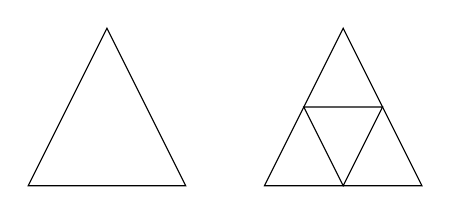
\begin{tikzpicture}
            % ������
            \draw (2, 1) -- (4, 1) -- (3, 3) -- cycle;
            \draw (5, 1) -- (6, 3) -- (7, 1) -- cycle;
            \draw (5.5, 2) -- (6.5, 2) -- (6, 1) -- cycle;
          \end{tikzpicture}
          \caption{ȫ�ּ���һ�ε�����}
        \end{minipage}
        \begin{minipage}[t]{0.6\textwidth}
          \centering
          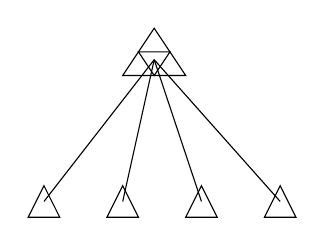
\begin{tikzpicture}
            %���������
            \draw (1.0, 0.0) -- (1.2, 0.4) -- (1.4, 0.0) -- cycle;
            \draw (2.0, 0.0) -- (2.2, 0.4) -- (2.4, 0.0) -- cycle;
            \draw (3.0, 0.0) -- (3.2, 0.4) -- (3.4, 0.0) -- cycle;
            \draw (4.0, 0.0) -- (4.2, 0.4) -- (4.4, 0.0) -- cycle;
            \draw (2.6, 2.4) -- (2.2, 1.8) -- (3.0, 1.8) -- cycle;
            \draw (2.4, 2.1) -- (2.6, 1.8) -- (2.8, 2.1) -- cycle;
            %������
            \draw (2.6, 2.0) -- (1.2, 0.2);
            \draw (2.6, 2.0) -- (2.2, 0.2);
            \draw (2.6, 2.0) -- (3.2, 0.2);
            \draw (2.6, 2.0) -- (4.2, 0.2);
          \end{tikzpicture}
          \caption{���ļ����Ŵ���}
        \end{minipage}
      \caption{�����Ŵ����ṹ}
      \label{fig::hgrometrytree}
    \end{figure}


\section{����~Krylov ���}
  ��~$\left(\{\phi_j \}_{j = 1}^n, 0 \right)^T$ �� ~$\left(0, \{\phi_j\}_{j = 1}^n\right)^T$ ���ٶȿռ�~$\mathbf{X}^h$ ������Ԫ��������ͬʱ~
  $\{\psi_k\}_{k = 1}^m$  Ϊѹ���ռ�~$P^H$ ������Ԫ��������$t_{n + 1}$ ʱ���ٶ���ֵ��ķ�����ʽ~$\vec{u}_h^{n + 1} = (u_h^{x, n + 1},
  u_h^{y, n + 1})^T$��$t = t_{n + 1}$ ��ѹ����ֵ��Ϊ ~$\vec{p}_H^{n + 1}$������дΪ��
  \begin{equation}
    u_h^{x, n + 1} = \sum_{j = 1}^{n_u} \alpha_j^{x, n + 1} \phi_j,
    \qquad u_h^{y, n + 1} = \sum_{j = 1}^{n_u} \alpha_j^{y, n + 1}
    \phi_j \qquad p_H^{n + 1} = \sum_{k = 1}^{n_p}\alpha_k^{p, n + 1}
    \psi_k.
    \label{eq::basis_fun}
  \end{equation}

  ��~\eqref{eq::basis_fun} ��������ʽ
  ~\eqref{eq::NS_weak_form} �У����Եõ�һ���������⣺
  \begin{equation}
    \left[
      \begin{array}{lll}
        \frac{1}{dt} M + \nu A + N & 0 & B_x^T \\
        0 & \frac{1}{dt} M +\nu A + N  & B_y^T \\
        B_x & B_y & 0
      \end{array}
    \right]
    \left[
      \begin{array}{c}
        \alpha^{x, n + 1} \\
        \alpha^{y, n + 1} \\
        \alpha^{p, n + 1}
      \end{array}
    \right] =
    \left[
      \begin{array}{c}
        f_x \\
        f_y \\
        0
      \end{array}
    \right],
    \label{eq::linear_system}
  \end{equation}
  ע�⵽ɢ�Ⱦ��� ~$B = [Bx, By]$ Ϊ
  \begin{eqnarray}
    B_x := [B_x]_{kj} = -\left(\psi_k, \frac{\partial \phi_j}{\partial
        x} \right), k = 1, \cdots, n_p, j = 1, \cdots, n_u, \\
    B_y := [B_y]_{kj} = -\left(\psi_k, \frac{\partial \phi_j}{\partial
        y} \right), k = 1, \cdots, n_p, j = 1, \cdots, n_u.
  \end{eqnarray}
  ��Ϊ�ٶȵ�Ԫ�ϵĻ�������ѹ����Ԫ�ϵĻ�����������ͬһ�������ϣ�����װ�����~$B$ ������һ����Ȼ�Ĺ��̡�����Ҫ���������ᵽ���ٶȵ�Ԫ��ѹ����Ԫ��
  ��~$1-1$ ���������ǿ��Խ���ֻ���ٶȺ�ѹ����Ԫ�ϵ�����Ԫ������װ��~$B$��ƴװ~$B^T$ �Ĺ������ơ�
  ���Ƕ��� ~$F_\nu^{n + 1} = \frac{1}{dt} M + \nu A + N$������
  \begin{eqnarray}
    M := &[M]_{ij} =& \left( \phi_i, \phi_j \right),\quad  i,j = 1, \cdots,
    n_u, \\
    A := &[A]_{ij} =& \left( \nabla \phi_i, \nabla \phi_j \right), i,j =
    1, \cdots, n_u, \\
    N := &[N]_{ij} =& \left(\vec{u}_h^n, \nabla \phi_i, \phi_j \right),
    i,j = 1, \cdots, n_u.
  \end{eqnarray}

  Ϊ�˸�Ч��������Է�����~\eqref{eq::linear_system} ��������Ԥ������~GMRES(generalized minimal residual algorithm)��Ϊ���������~\cite{elman2005finite}
  �п��ǵĿ�����Ԥ����~$\mathcal{P}$ �������£�
  \begin{equation}
    \mathcal{P} =
    \left(
      \begin{array}{lll}
        F & 0 & B_x^T \\
        0 & F  & B_y^T \\
        0 & 0 & S
      \end{array}
    \right),
  \end{equation}
  ���� ~$S = B_xF^{-1}B_x^T + B_yF^{-1}B_y^T$ �� ~schur  ������Ԥ��������Ҫ��ɽ��ƾ�������棬ʵʩ~$\mathcal{P}^{-1}$ �Ĺ��̷�Ϊ������
  ��һ�������~schur ����ϵͳ���ڶ�����������������ĸ�~$F$ �йص�ϵͳ��ֱ�����~schur ���ķ������Ƿdz���ʱ�ģ���Ϊ��ϵ�����������һ����
  �������ԣ���ʵ�ʵļ����У��ҵ�~schur ���Ľ��ƾ���Ȼ���ý��ƾ������~schur ��������������⡣�� ~$2$ �����ᵽ~PCD �н���~schur  ���ľ���Ϊ��
  \begin{equation}
    S_* = A_p F_p^{-1} Q_p,
    \label{eq::PCD}
  \end{equation}
  ����~$A_p, F_p$ �� ~$Q_p$ ȫ��������ѹ���ռ��ϡ� $Q_p$ ��ѹ���������� $A_p$ ��ѹ���նȾ���$F_p$ �Ƕ�����ɢ�������Ƿֱ���Ϊ��
  \begin{eqnarray}
    F_p := [F_p]_{ij} = \nu (\nabla \psi_i, \nabla \psi_j) +
    (\vec{u}_h^n \cdot \nabla \psi_i, \psi_j), \quad i,j = 1, \cdots, n_p, \\
    A_p := [A_p]_{ij} = (\nabla \psi_i, \nabla \psi_j)\quad i,j = 1, \cdots,
    n_p.
    \label{eq::pcd_mat}
  \end{eqnarray}
  ��
  \begin{equation}
    W_p^n := [W_p^n]_{ij} = (\vec{u}_h^n \cdot \nabla \psi_i,
    \psi_j), \quad i,j = 1, \cdots, n_p,
  \end{equation}
  ��ô~$F_p$ ���Ա�����д�ɣ�
  \begin{equation}
    F_p = \nu A_p + W_p^n.
  \end{equation}
  ����ʵʩ~PCD Ԥ����ͨ��
  \begin{equation}
    S_*^{-1} = Q_p^{-1} F_p A_p^{-1}.
  \end{equation}
  ��ȷ��~PCD Ԥ�������Ӷ���Ϊ
  \begin{equation}
    \mathcal{M}^{-1} =
    \left(
      \begin{array}{lll}
        F^{-1} & 0 & B_x^T \\
        0 & F^{-1} & B_y^T \\
        0 & 0 &S_*^{-1}
      \end{array}
    \right)
  \end{equation}
  ���Ƿ���������Ԥ�����������̣���~$V^d = \mathcal{M}^{-1} V^s$��
  ����
  \begin{equation}
    V^d = (V_x^d, V_y^d, V_p^d)^T, V^s = (V_x^s, V_y^s, V_p^s)^T.
  \end{equation}
  ��һ��������⣺
  \begin{equation}
    V_p^d = S_*^{-1} V_p^s = Q_p^{-1} F_p A_p^{-1} V_p^s.
    \label{eq::solve_schur}
  \end{equation}
  �����а�������������������~$Q_p^{-1}$ �� ~$A_p^{-1}$���������ǿ�����Ϊ��Ⲵ��������ƵĴ������������������ʵ����⡣
  �ڶ��������������ֶ������������ȥ���
  \begin{equation}
    \begin{aligned}
      V_x^d = F^{-1} (V_x^s - B_x^T V_p^d), \\
      V_y^d = F^{-1} (V_y^s - B_y^T V_p^d).
    \end{aligned}
    \label{eq::solve_velocity}
  \end{equation}
  ��~\eqref{eq::solve_schur}  �� ~\eqref{eq::solve_velocity} �еĽ�ϲ���һ�𣬾͵õ���Ҫ���� ~$V^d$.

  ��ʵ�ʵļ����У����ǶԾ���~$F$�� $F_p$�� $Q_p$ �� ~$A_p$ ����⣬���ù̶��ļ������������������(algebraic multi-grid)�����澫ȷ��⡣��
  ���ǵ�����~PCD �����������õĶ����������������~AFEPack \cite{AFEPack} (һ������Ӧ����Ԫ��)�С���~(\cite{elman2005finite}��
  ��10��)�У���ֵ����˵����~PCD Ԥ�����ĸ�Ч��\cite{elman2011fast} һ�Ľ�~PCD Ԥ��������Ӧ�õ�~bouyancy �����������ϡ������ǵ���ֵʵ���У����������
  ~\eqref{eq::pcd_mat} �е�
  \begin{equation}
    F_p = \nu A_p + W_p^n,
  \end{equation}
  ��~$A_p$ ǰ���ϵ�� ~$\nu$ ȥ�����ᷢ��~GMRES~�ĵ�����������١����Dz��� ~\cite{elman2009boundary} ����~Neumann �߽��ϵĴ�������~$F_p$ �� ~$A_p$ �ķ����������
  ���Ч�ʡ�$F_p$ ��Ҫ�ڱ߽�~$\partial \Omega = \partial \Omega_D \cup \partial \Omega_N$ ������߽�����
  \begin{equation}
    \nu \frac{\partial p_h}{\partial n} + (\vec{w}_h \cdot \vec{n})
    p_h = 0.
    \label{eq::bc_Fp}
  \end{equation}
  ͨ���� ~$2$ ���е�Ԥ������������֪���ڳ����߽�
   ~$\partial \Omega_N$ �ϣ���ɢ��ѹ�� ~$p_h$ ��Ҫ����һ����ε�~Dirichlet �߽�������
   ����~$\Omega_D$ �ϣ�ѹ��~$p_h$ Ҫ������Ȼ���� ~$\frac{\partial p_h}{\partial n} = 0$���Ǿ���ζ��������Dirichlet�߽��ϣ���~$A_p$ ����ȡ�κβ�����
  ����֪�����ڷ�ǻ���������еı߽���~$\vec{w}_h \cdot \vec{n} = 0$������~\eqref{eq::bc_Fp} �����˻���
  \begin{equation}
    \frac{\partial p_h}{\partial n} = 0.
  \end{equation}
  �����ζ�����������еı߽�~$\partial \Omega$ �ϣ���~$F_p, A_p$ ����ȡ�κβ�����
  �ڱ����У����ǽ�~PCD Ԥ��������Ӧ�õ��ƶ���������Ԫ����������Ч�����~Navier-Stokes ����~\eqref{eq::linear_system}��
\section{�ƶ��������}
  \subsection{�����ƶ�������}
     �ٵ�~$3$ ����������ϸ�Ľ��ܹ��ƶ�����IJ��ԣ���һ���м�Ҫ����һ�¡���~$t = t_{n}$ ʱ�̣����ǻ������ֵ�� ~$\vec{u}_h^{(n)}, p_H^{(n)}$ ��~$t_n$ ʱ�̵�
     ���� ~$\mathcal{T}_h^n$ �ϡ����Ǹ���~\cite{di2005moving} �еķ������ñ���ɢ��Ϊ0�IJ�ֵ������~$\mathcal{T}_h^n$ �ϵ���ֵ���ֵ��~$t_{n + 1}$ ʱ�̵�����
     ~$\mathcal{T}_h^{(n + 1)}$ �ϡ��򵥵���˵���ܹ���Ϊ������
     \begin{enumerate}[step 1]
     \item ��ȡ���ƺ����� ��~$m = 1/G$������~$G$ �ǿ��ƺ��������������Ŀ��ƺ���
       \begin{equation}
         \centering
         G = \sqrt{1 + \alpha |\omega|^\beta},
         \label{eq::monitor_vorticity}
       \end{equation}
       ���� ~$\omega = \nabla \times \vec{u}$�� $\alpha, \beta$
       ���������ij������ڱ����У�$\beta = 2$ �бȽϵ�Ч����$\alpha$  ���ݲ�ͬ�����⣬ѡȡ��ͬ��ֵ��

     \item ��ȡ���������ϵ��ƶ��������
       \begin{equation}
         \begin{aligned}
           \nabla_{\vec{x}}(m \nabla_{\vec{x}} \vec{\xi}) &= 0,& \\
           \vec{\xi}|_{\partial \Omega} & = \vec{\xi}_b,&
         \end{aligned}
         \label{eq::logical}
       \end{equation}
       �����һ���µ��߼�����~$\mathcal{T}_c^*$��$\mathcal{A}^*$ ��Ϊ���Ľڵ㡣
       ���ǿ��Եõ��µ��߼�����ͳ�ʼ�߼�����~$\mathcal{T}_c^0(\mbox{�ڵ�Ϊ} \mathcal{A}^0)$
       ֮������
       \begin{equation}
         \delta \mathcal{A} = \mathcal{A}^0 - \mathcal{A}^*.
       \end{equation}
       ���ǿ��Ը���~$\delta \mathcal{A}$ ��������������λ��~$\delta X_i$��ͨ���ٳ���һ�����ij���~$\mu$
       ����������ӣ�
       \begin{equation}
         X_i^{(n + 1)} = X_i^{(n)} + \mu \delta X_i.
       \end{equation}
     \item ����ɢ��Ϊ~$0$ �IJ�ֵ��
       �����ƶ���������Ԫ��������ⲻ��ѹ���巽�̵�ʱ����Ҫ����ֵ���ֵ�Ĺ����б���ɢ��Ϊ~$0$����~\cite{di2005moving} �У�
       ��ֵ����������~$\mathcal{T}^{(n + 1)}$ �ϵ����·ֲ�����ͨ�����һ��������ճ��~Navier-Stokes ���̡�
       \begin{eqnarray}
         \begin{aligned}
           \frac{\partial \vec{u}}{\partial \tau} - \nabla_{\vec{x}}\vec{u}
           \cdot \delta \vec{x} & =  - \nabla \hat{p},& \\
           \nabla_{\vec{x}}\cdot \vec{u} & =  0,&
         \end{aligned}
         \label{eq::continous_update}
       \end{eqnarray}
       ���� ~$\delta \vec{x} := x^{\text{old}} - x^{\text{new}}$��
       $x^{\text{old}}, x^{\text{new}}$  �����������ϵ��������ꡣ$\tau$ ��һ������ʱ�䣬ͨ��ȡ��~$1.0$����Ϊ�����ٶ�~$\delta \vec{x}$
       ��Խ�С������ ~$\hat{p}$ ��һ����ʱ������Ϊ�˸�~\eqref{eq::NS_chap4} �е�ѹ��������������

       ~\eqref{eq::continous_update} ������ʽ��: Ѱ�� ~$(\vec{u}_h, \hat{p}_H) \in X_E^h \times P^H$ ʹ��
       \begin{eqnarray}
         \begin{aligned}
           \left( \partial_{\tau} \vec{u}_h - \nabla_{\vec{x}}\vec{u}_h
           \cdot \delta \vec{x}, \vec{v}_h \right) & =  \left( \hat{p}_H, \nabla
           \vec{v}_h \right), \quad \forall \vec{v}_h \in X_E^h,&  \\
           \left( \nabla_{\vec{x}} \cdot \vec{u}, q_H\right) & =  0, \quad \forall
           q_H \in P^H. &
         \end{aligned}
         \label{eq::semi_discreted_update}
       \end{eqnarray}

       �ڱ����У�������ʱ���������ʾ��ʽ��ɢ
       ~\eqref{eq::semi_discreted_update} ��
       \begin{eqnarray}
         \begin{aligned}
           \left ( \frac{\vec{u}_{h, *}^{(n)} - \vec{u}_h^{(n)}}{\delta
               t},
           \vec{v}_h \right) + \left( \delta \vec{x} \cdot \nabla
           \vec{u}_{h}^{(n)}, \vec{v}_h \right)  & =  \left(
           \hat{p}_{H, *}^{(n)}, \nabla \vec{v}_h \right), \quad
           \forall \vec{v}_h \in X_E^h. &\\
           \left( \nabla \cdot \vec{u}_{h, *}^{n}, q_H \right) & =  0, \quad
           \forall q_H \in P^H. &
         \end{aligned}
         \label{eq::full_discreted_update}
       \end{eqnarray}
       ����~$\vec{u}_h^{(n)}$ �� ~$p_H^{(n)}$ �Ƿ���~\eqref{eq::NS_chap4}
        �� ~$t = t_{n}$ ʱ�̵������ϼ������ֵ�⡣$\vec{u}_{h,*}^{(n)}$ �� ~$p_{h, *}^{(n)}$
      ����������~$\mathcal{T}^{(n + 1)}$ �ϣ�$t_n$ ʱ�̵���ֵ�⣬��һ���м������
     \end{enumerate}

   \subsection{��AMG Ԥ�������~\eqref{eq::full_discreted_update}}
   \eqref{eq::full_discreted_update} ����õ�һ������ϵͳ�� ����ϵ������Ϊ~$\mathcal{M}^p$���������£�
   \begin{equation}
     \mathcal{M}^p =
     \left(
       \begin{array}{lll}
         \frac{1}{\delta t} Q_p & 0 & B_x^T \\
         0 & \frac{1}{\delta t} Q_p & B_y^T \\
         B_x & B_y & 0
       \end{array}
     \right)
     \label{mat::moving}
   \end{equation}
   ��������֪������~$\mathcal{M}^p$ ��~schur������Ϊ��
   \begin{equation}
    M_S = B_x Q_p^{-1} B_x^T + B_y Q_p^{-1} B_y^T.
   \end{equation}
   ���ݵ�~$2$ �£���������~LBB �����Ļ��Ԫ���ƣ����߽�����ȫ���Ƿ������߽�ʱ��$M_S$ �Ǹ�ѹ���ռ�ĸնȾ���
   ~$A_p$ �׵ȼ۵ġ�������ǿ����� ~$A_p$ ����Ϊ~Schur ������Ľ��ƾ�����ô���ǿ���ѡȡ
   \begin{equation}
     \mathcal{K} =
     \left(
       \begin{array}{lll}
         Q_p & 0 & B_x^T \\
         0 & Q_p & B_y^T \\
         0 & 0 & M_S^*
       \end{array}
     \right),
     \label{eq::updateSolution_precond}
   \end{equation}
   ����Ϊ~\eqref{mat::moving} �Ŀ�Ԥ������������ ~$M_S^* = A_p$ ���� ~$M_S^* =
   \frac{1}{\nu} A_p$������ѡ��ͬ��~$M_S^*$ ����Ϊ~schur ������Ľ��ƾ���
   ���Ա����Ч�ʵIJ�������ǵ�ʵ�ʼ����У�$\frac{1}{\nu}A_p$ Ҫ�� ~$A_p$ Ч��Ҫ�ߡ�
   ��������/�������⣬$A_p$ ��Ҫ��~Neumann �߽�������һЩ�޸�����߼���Ч�ʡ��ڳ����߽�
   ~$\partial \Omega_N$ �ϣ���Ҫ����ѹ�� ~$p_h = 0$��
   ����~$\Omega_D$ �ϣ�ѹ��~$p_h$  Ҫ���� ~$\frac{\partial p_h}{\partial n} = 0$��
   ����������~Dirichlet �߽��ϣ���~$A_p$ ����ȡ�κβ�����ϸ�ڿ��Բο�~\cite{elman2009boundary}��
   ע�⵽��һ���������ƶ������еľ��� $M, B_x^T, B_y^T, B_x, B_y, A_p$ ����Ҫ���¹�����

   �����ǵ��㷨�У�PCD Ԥ������~GMRES ��Ϊ�������ϵͳ~\eqref{eq::linear_system} ���������
   ���Ƕ���~GMRES~������ֹͣ׼��Ϊ
   \begin{equation}
     ||r^{(k)}||  \leq 10^{-6} ||r^{(0)}||
   \end{equation}
   ���� ~$r^{(k)}$ ������ϵͳ~\eqref{eq::linear_system} �IJв$r^{0}$ ��~\eqref{eq::linear_system} ���Ҷ���IJв
   ���Ϊ������ر������ǵ��㷨�����Ǹ�������ͼ���㷨 ~\ref{alg::solve_AMG}��

      \begin{algorithm}
        \caption{�ƶ���������Ԫ�������~Navier-Stokes}
        \begin{algorithmic}[1]
          \State ��~AMG Ԥ�����������̬��~Stokes ��������ó�ֵֵ ~$\vec{u}_h^{(0)}, p_H^{(0)}$��
          \While {$t_n < T$}
          \State ��~$\triangle_p^{(n)}$ �ϣ��� ~$\vec{u}_h^{(n)}, p_H^{(n)}$  ������ƺ���������ͨ��������ӳ��~\eqref{eq::logical} �����
                 �µ��߼�����~$\vec{\xi}^*$�� \label{state::monitor_chap4}
          \State �ж� ��� ~$\vec{\xi}^* - \vec{\xi}^{(0)}$ �� ~$L_2~$ �����Dz��DZ�������С�����ǣ����������������
                 ���� \ref{state::start_chap4} - \ref{state::end_chap4}��
          \State ��~$\vec{\xi}^* - \vec{\xi}^{(0)}$ ֮������������ѹ������~$\triangle_p^{(n)}$ �����������ϵ��ƶ���~$\delta \vec{x}$��
                 \label{state::start_chap4}
          \State ���ٶ����� ~$\triangle_v^{(n)}$ �ϣ���AMGԤ����������ⷽ�� ~\eqref{eq::full_discreted_update}  ����ȡ�м����
                 ~$\vec{u}_{h, *}^{(n)}, p_{H, *}^{(n)}$��
          \State ����ѹ������ ~$\triangle_p^{(n)}$ �� ~$\triangle_p^{(n +
                 1)}$ �������ü����Ŵ����ṹ��ͬ�� ~$\triangle_v^{(n)}$ ��
                 ~$\triangle_v^{(n + 1)}$��
          \State �ص� \ref{state::monitor_chap4}�� \label{state::end_chap4}

          \State ��~AMG Ԥ������������� ~Navier-Stokes ���� ~\eqref{eq::linear_system} ���Ӷ����������~$\triangle_v^{(n + 1)}$ �� ~$\triangle_p^{(n
                 + 1)}$ �ϵ���ֵ�� ~$\vec{u}_h^{(n + 1)}, p_H^{(n + 1)}$��
          \State $n = n + 1$
          \EndWhile
        \end{algorithmic}
        \label{alg::solve_AMG}
      \end{algorithm}


% ----------------------------------------------------------------------------------------
%	SECTION 6
% ----------------------------------------------------------------------------------------
\section{��ֵ����}
      ������������ֵ������չʾ���ǵķ�������ʵ�ʵļ�������У����Dz�����̬��~Stokes ���̵Ľ���Ϊ~Navier-Stokes ���̵ij�ʼֵ��
      �߽��������ø�~Navier-Stokes ����һ�¡������ǵ��㷨�У���ʼ������������߼�������һ�µġ�������ƶ�Ч���Լ���ֵ����
      ����չʾ���������ǵĴ����ǻ�������Ԫ��~AFEPack��

     \subsection{��ǻ������}
       ���ǿ��Ǿ������������򻯵ķ�ǻ�������ǵļ���������~$\Omega = [-1, 1] \times [-1, 1]$��ճ��ϵ����~$Re = 2000$��Dirichlet
       �߽��������������еı߽�~$\partial \Omega$ �ϡ��ڶ������ϣ��ٶ�~$\vec{u} = (1 - x^4, 0)^T$���޻�������������~$\partial \Omega$
       ���������֡�

       �����ǵ��ƶ������У�����ѡȡ����~\eqref{eq::monitor_vorticity} Ϊ���ƺ���������ȡ��~$\alpha = 0.5, \beta = 2.0$ ʱ�����ƶ�Ч��
       �ȽϺá���ͼ~\ref{fig::cavity_flow_mesh} ��չʾ���Ƿ�չ����̬���ƶ������Լ������ĵȸ��ߡ����ǿ��Կ����������ڶ����ߺ��ұ߽߱�
       ����Щ�ط����������Ƚϴ�ĵط����ٶȵ���������ͼ~\ref{fig::cavity_flow_streamline}��
       ��ͼ~\ref{fig::cavity_flow_divergence} �У����ǶԱ��˾���������ƶ������£��ٶ�ɢ�ȴ�С��������֣��ٶ�ɢ��ֵ���ƶ������±�
       ��������ҪСһ�룬��˵���ˣ��ƶ������Ч���Ⱦ�������Ҫ�á�
       \begin{enumerate}
           \item �Ա���� ~\eqref{eq::linear_system} ��~GMRES �ĵ���������

                ��ͼ ~\ref{fig::cavity_compare_Fp} �����ǿ��Կ�������~PCD Ԥ������ѡȡ ~$F_p = A_p + W_p^n$ ��Ҫ��~GMRES �ĵ��������� ~$F_p = \nu A_p + W_p^n$ �١������ڱ� ~\ref{tab::comparation_GMRES_steps} �жԱ��ˣ���~ AMG �� ~ILU����Ԥ�����������ʱ��GMRES ��ƽ���������������Ƿ���
                ~AMG Ԥ������~ILU Ч�ʸߺܶࡣ
           \item �Ա���� ~\eqref{eq::full_discreted_update} ��~GMRES �� ����������

               �� ~\ref{tab::GMRES_steps_update}�����ǶԱȲ�ͬ��Ԥ��������
               ~$M_S^*$ ��Ӧ��ƽ����~GMRES ����������������֣������ ~\ref{eq::full_discreted_update} ʱѡȡ ~$M_S^* = \frac{1}{\nu} A_p$��GMRES ������������ٷdz����ԣ���Ա� ~$M_S^* = A_p$��
       \end{enumerate}

       \begin{figure}[!htbp]
         \begin{center}
             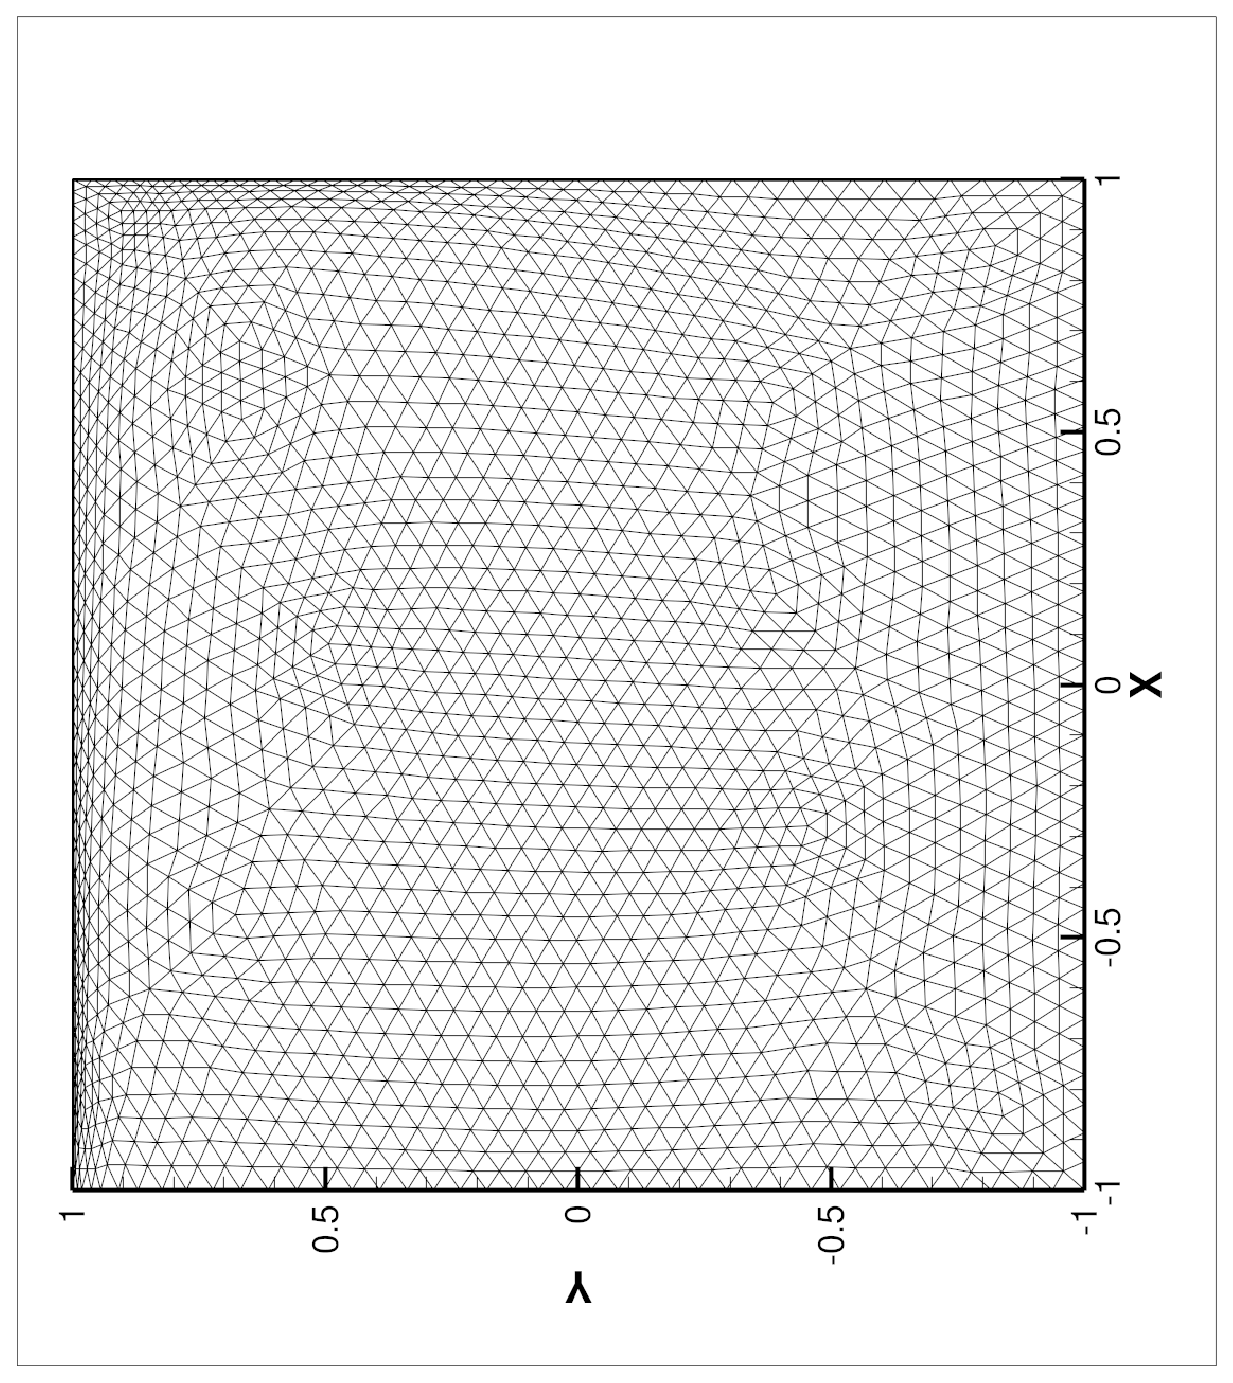
\includegraphics[width = 0.43\textwidth, angle = -90]{picture/second/cavity_flow_data/moving_mesh_20.eps}
             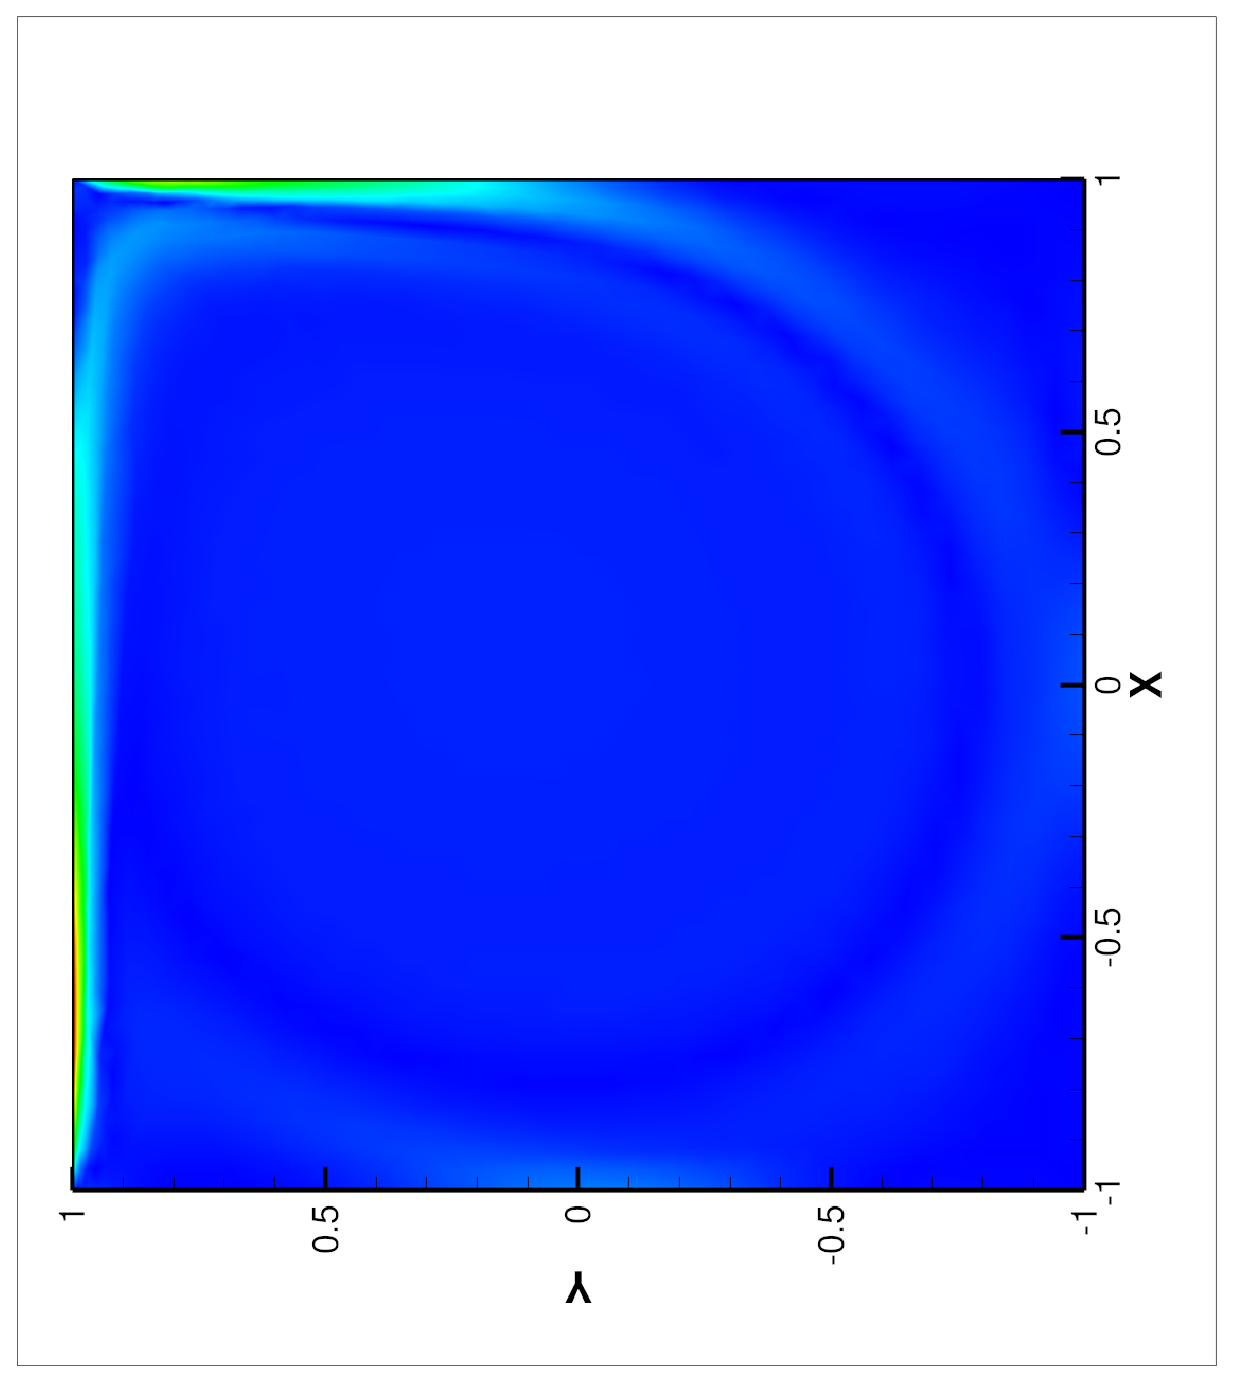
\includegraphics[width = 0.43\textwidth, angle = -90]{picture/second/cavity_flow_data/vortex_mesh20.eps}
        \end{center}
        \caption{  ��ǻ�������ƶ������ң������ĵȸ��ߣ�ѹ������ ~$20 \times 20$��$Re = 2000$��}
        \label{fig::cavity_flow_mesh}
       \end{figure}

       \begin{figure}[!htbp]
         \begin{center}
             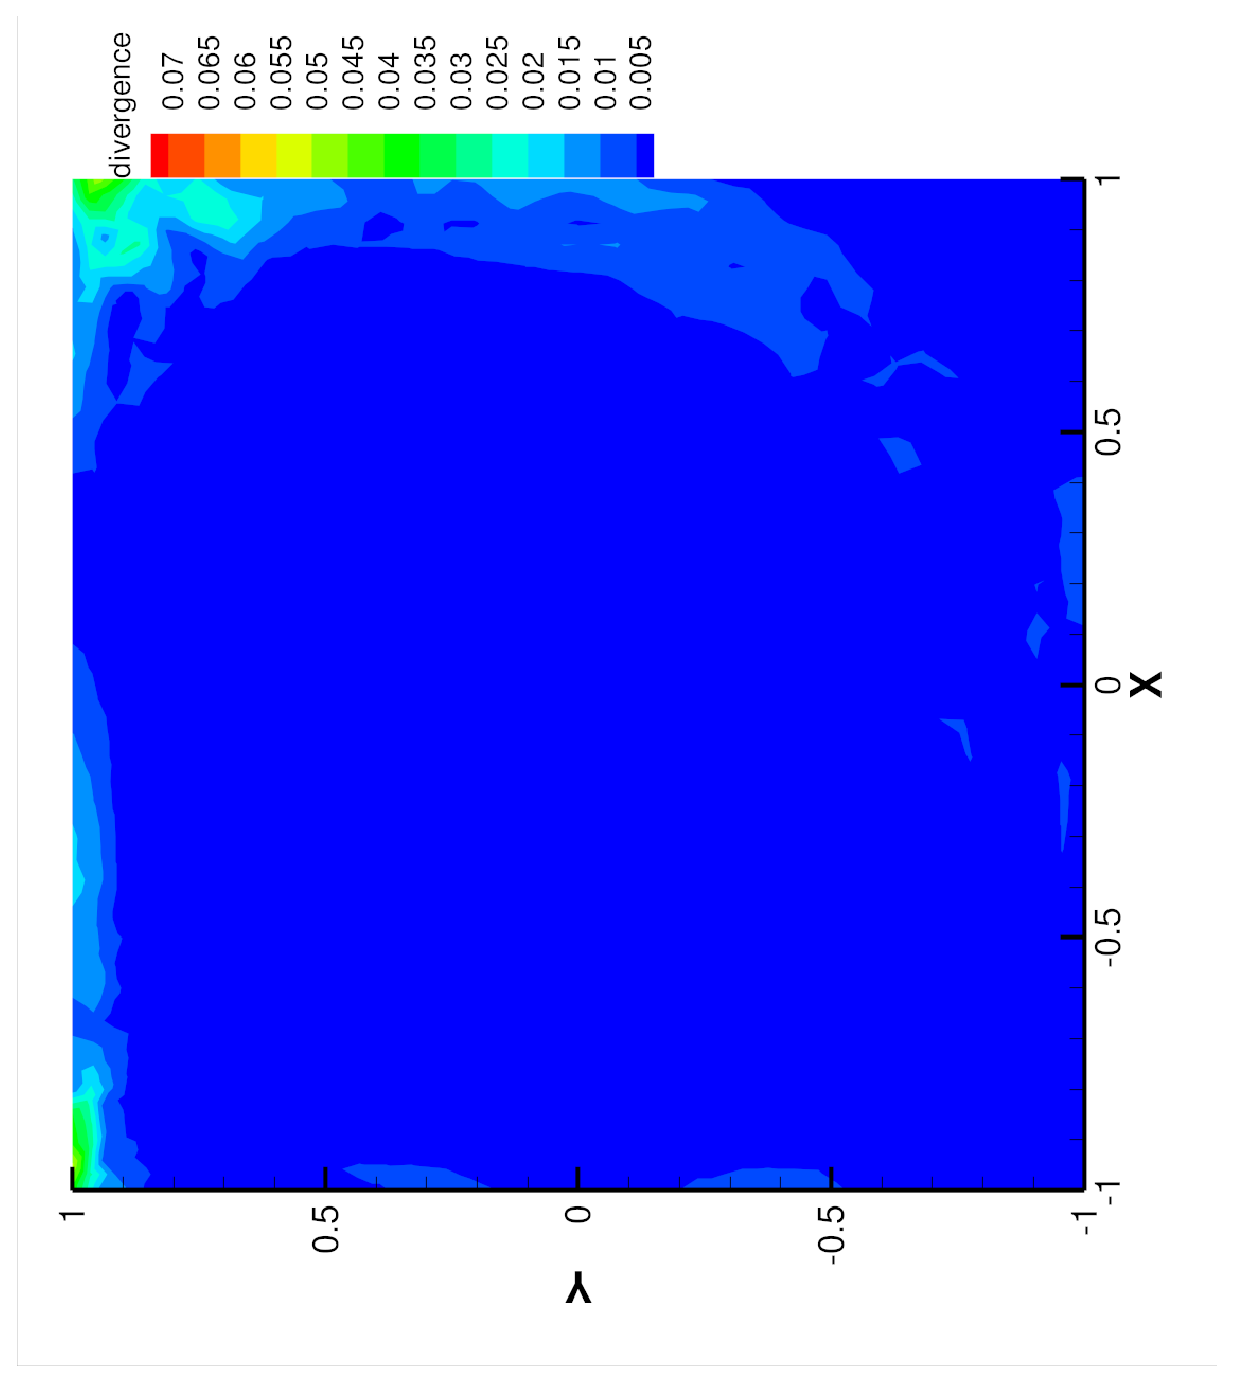
\includegraphics[width = 0.43\textwidth, angle = -90]{picture/second/cavity_flow_data/divergence_uniform_1.eps}
             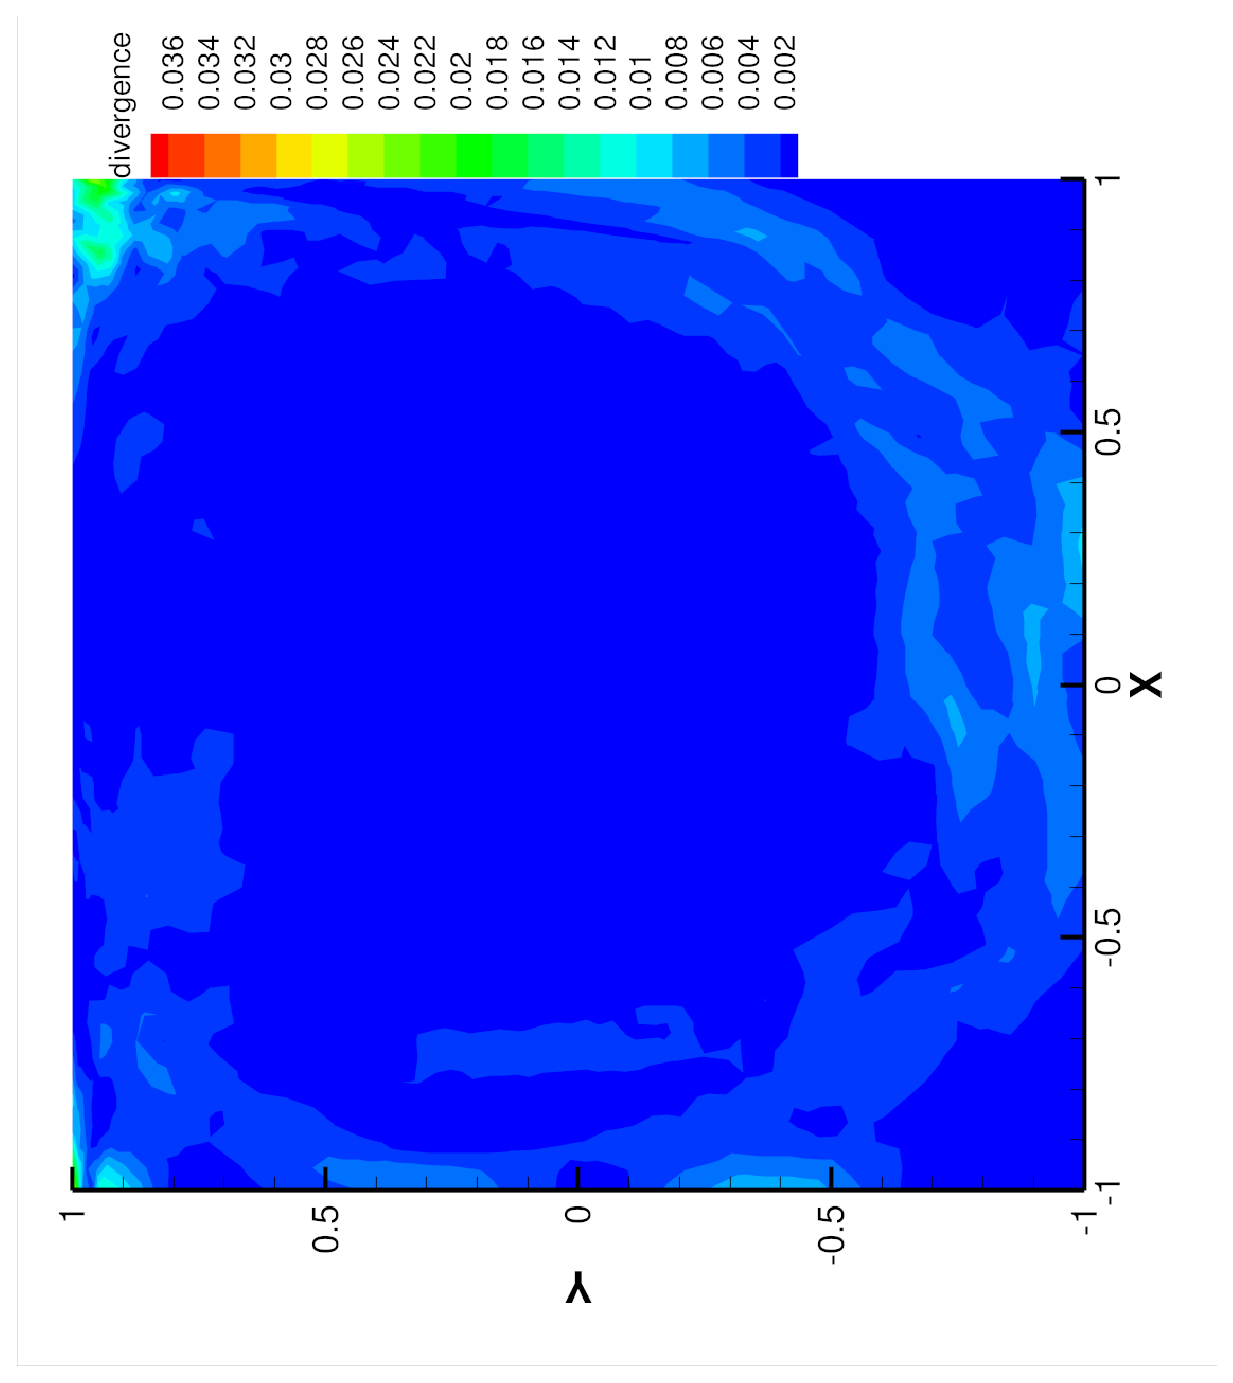
\includegraphics[width = 0.43\textwidth, angle = -90]{picture/second/cavity_flow_data/divergence_moving_1.eps}
        \end{center}
        \caption{  ��ǻ�����ٶȵ�ɢ�ȵȸ��ߣ��󣺾��������ң��ƶ�����ѹ������ ~$20 \times 20$��$Re = 2000$��}
        \label{fig::cavity_flow_divergence}
       \end{figure}

       \begin{figure}[!htbp]
         \begin{center}
             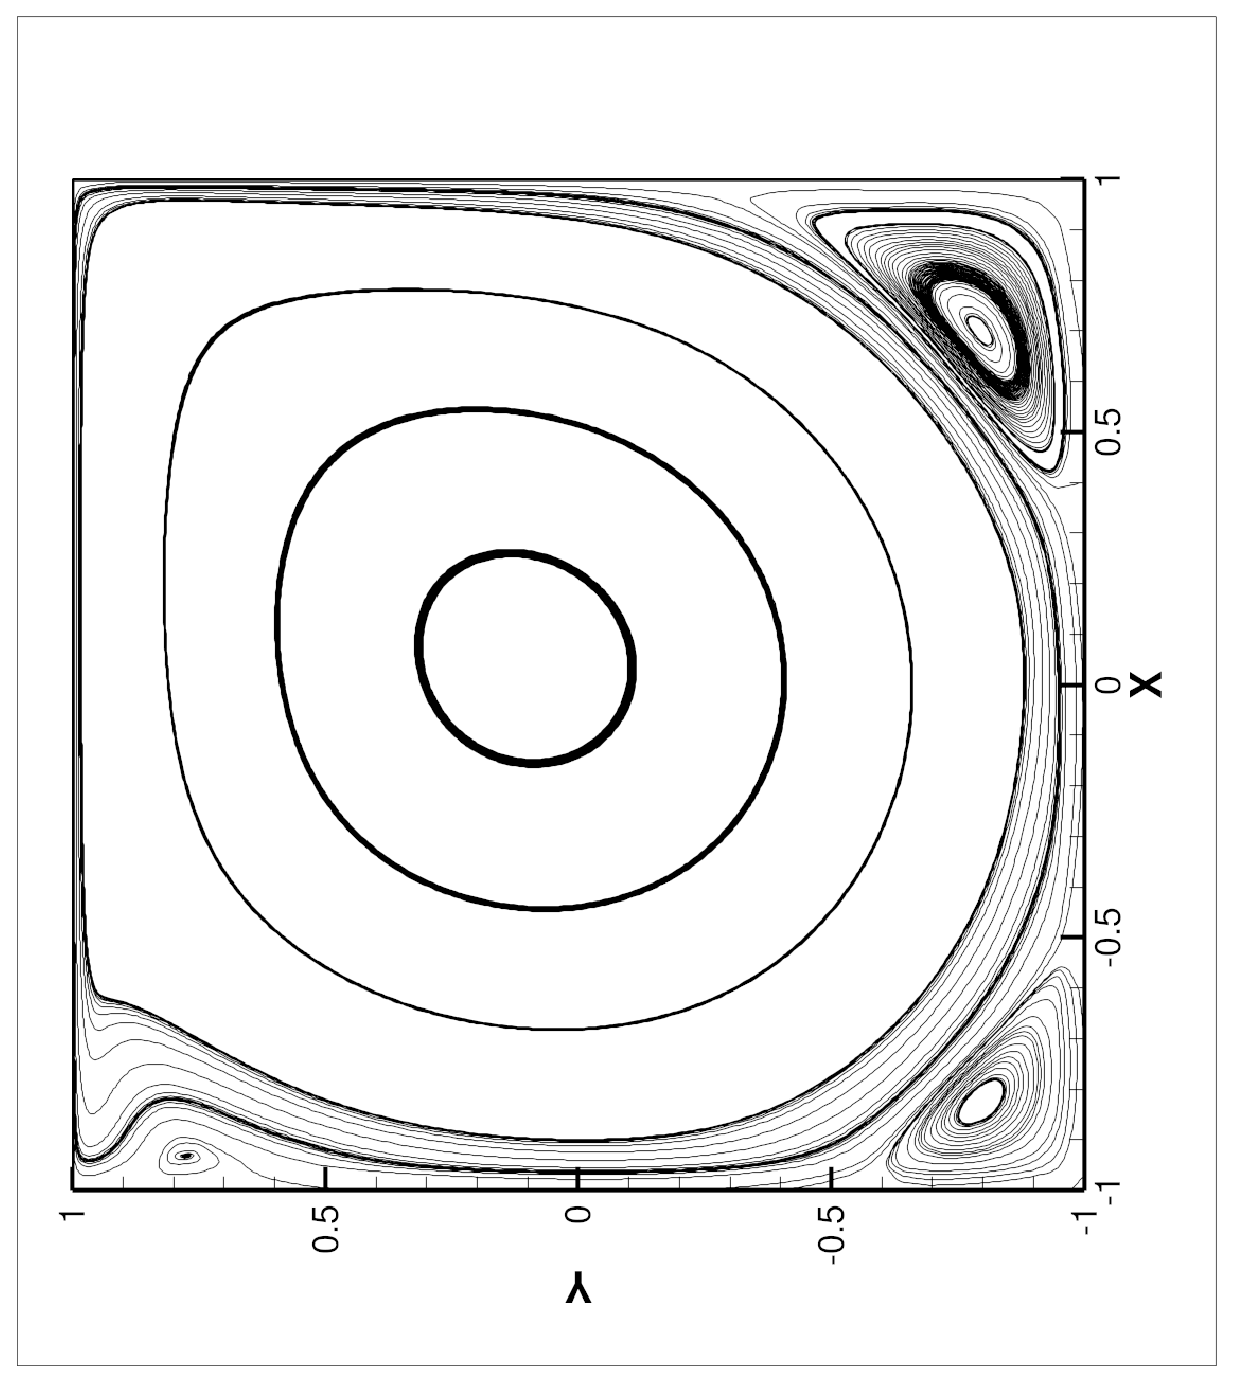
\includegraphics[width = 0.43\textwidth, angle = -90]{picture/second/cavity_flow_data/streamline_mesh20.eps}
        \end{center}
        \caption{  ��ǻ���������ߣ�ѹ������ ~$20 \times 20$��$Re = 2000$��}
        \label{fig::cavity_flow_streamline}
       \end{figure}

       \begin{figure}[!htbp]
         \begin{center}
           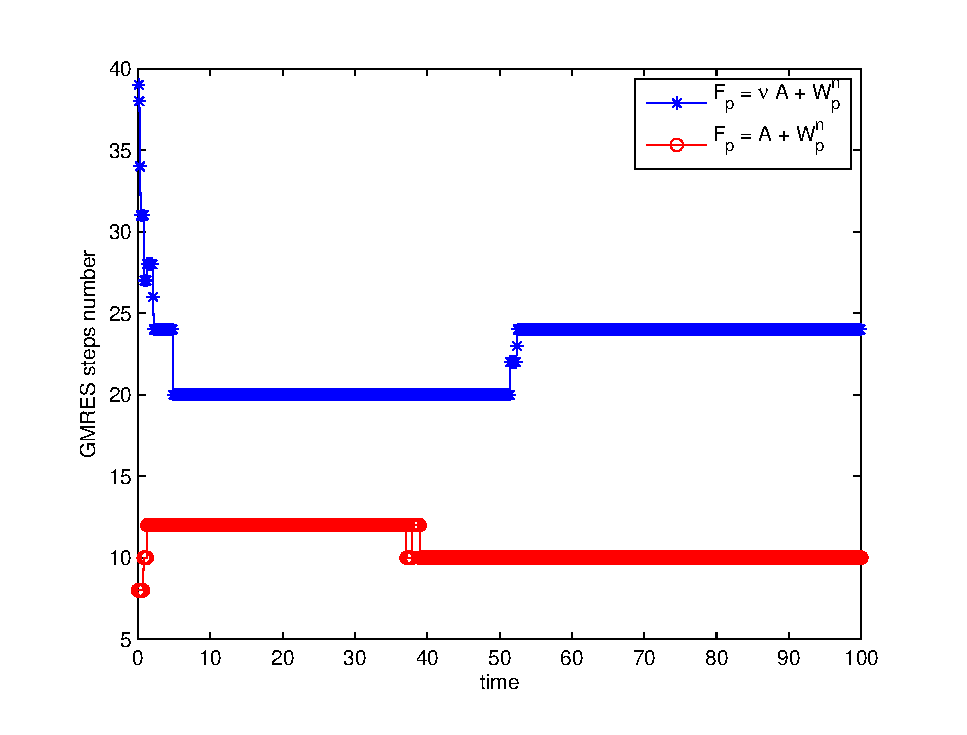
\includegraphics[width = 0.55\textwidth, angle = 0]{picture/second/cavity_flow_data/Fp_comparation_mesh20.eps}
        \end{center}
        \caption{  ��ǻ�����Ա���~PCD Ԥ�������ò�ͬ�� ~$F_p$ �����~\eqref{eq::linear_system} ʱ��GMRES �ĵ���������
        ѹ������ ~$20 \times 20$�� $Re = 2000$��}
        \label{fig::cavity_compare_Fp}
       \end{figure}

       \begin{table}[!htbp]
         \centering
         \begin{tabular}{ccc}
           \hline
           \multirow{2}{*}{ѹ������}  & \multicolumn{2}{c}{GMRES ��ƽ����������} \\
           \cline{2-3}
                           & $AMG$ & $ILU$ \\ \hline
           $20 \times 20$   &      $10.8$           &     $107.5$
           \\ \hline
           $40 \times 40$   &      $16.01$             &     $307.33$
           \\ \hline
           $80 \times 80$   &     $27.18$              &     $>500$
           \\ \hline
         \end{tabular}
         \caption{  ��ǻ��: �Ա��� ~AMG �� ~ILU Ԥ��������� ~\eqref{eq::linear_system} ʱ��GMRES �ĵ���������$Re = 2000$��}
         \label{tab::comparation_GMRES_steps}
       \end{table}

       \begin{table}[!htbp]
         \centering
         \begin{tabular}{cccc}
           \hline
           \multirow{2}{*}{ѹ������}   & \multicolumn{2}{c}{GMRES ��������} \\
           \cline{2-3}
                           & $M_S^* = \frac{1}{\nu}A_p $& $M_S^* = A_p$ \\ \hline
           $20 \times 20$  &      $4.96$           &     $13.19$
           \\ \hline
           $40 \times 40$  &      $10.99$           &     $42.36$
           \\ \hline
         \end{tabular}
         \caption{��ǻ�����Ա��ò�ͬ��Ԥ�������� ~$M_S^*$����� ~\eqref{eq::full_discreted_update} ʱ��GMRES ƽ������������$Re = 2000$��}
         \label{tab::GMRES_steps_update}
       \end{table}

%       \begin{figure}[!htbp]
%         \begin{center}
%             \includegraphics[width = 0.43\textwidth, angle = -90]{picture/second/second/cavity_flow_data/moving_mesh.eps}
%             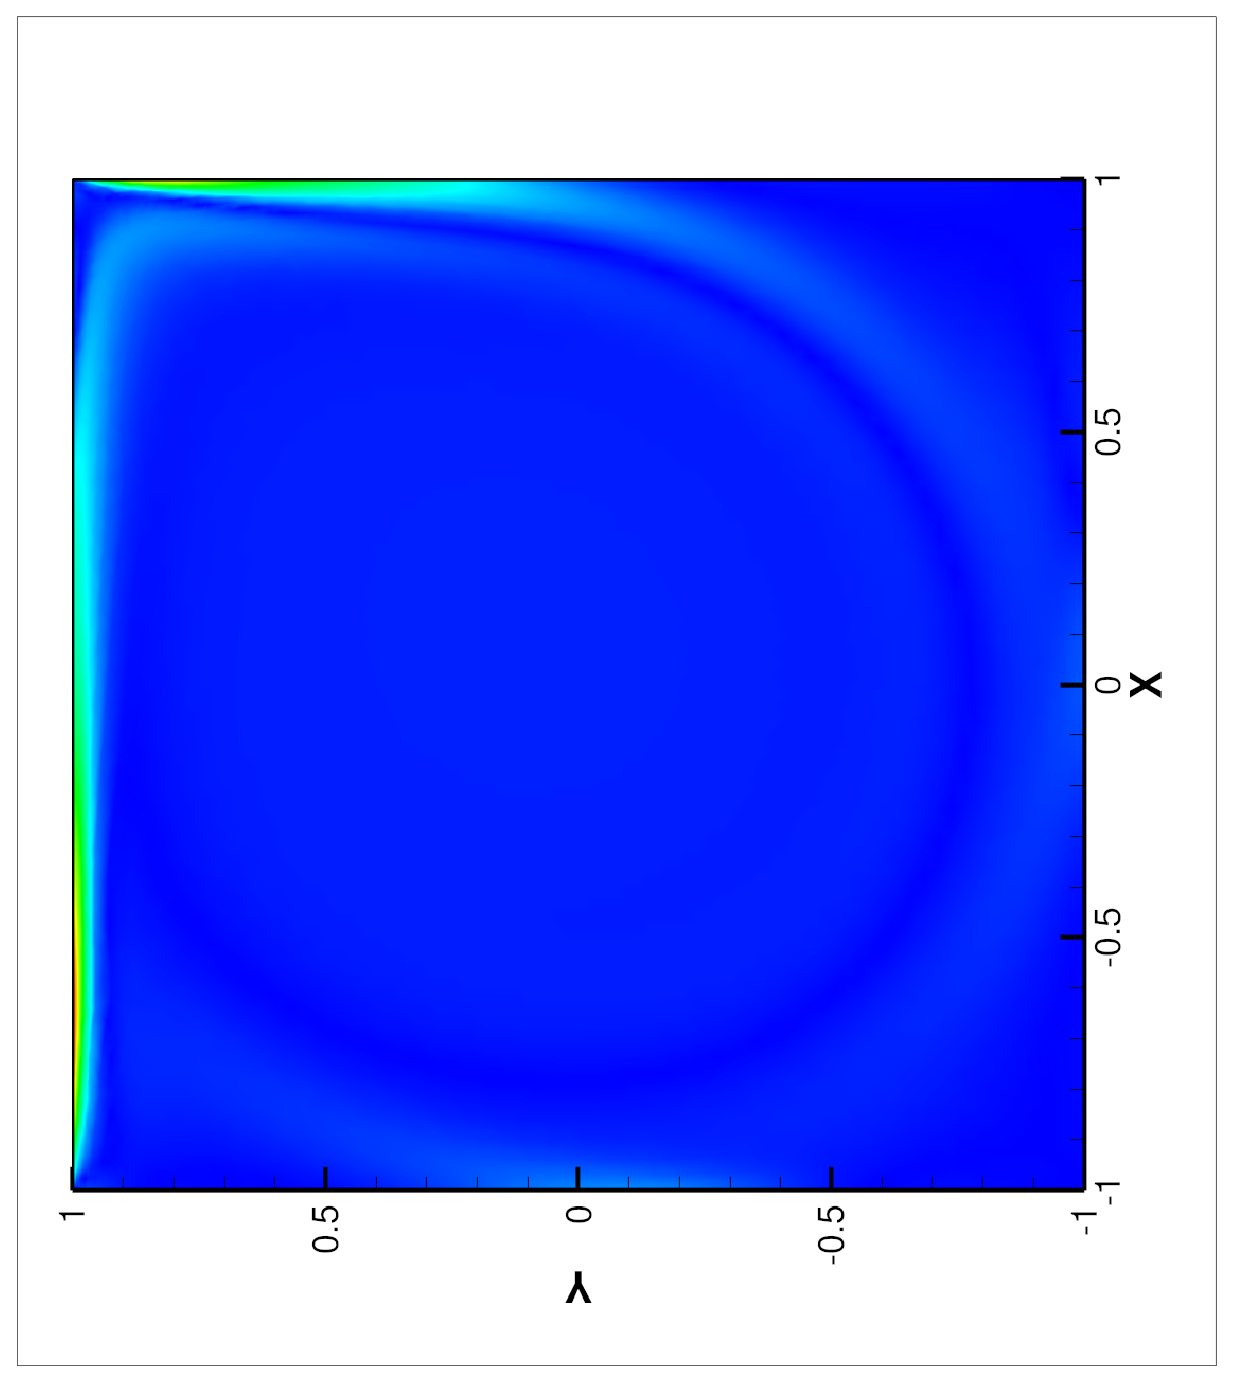
\includegraphics[width = 0.43\textwidth, angle = -90]{picture/second/second/cavity_flow_data/vortex.eps}
%        \end{center}
%        \caption{  Cavity flow, left: mesh, right: vorticity
%          contour, pressure mesh $40 \times 40$, $\nu = 0.001$.}
%        \label{fig::cavity_flow_mesh}
%       \end{figure}
%
%       \begin{figure}[!htbp]
%         \begin{center}
%             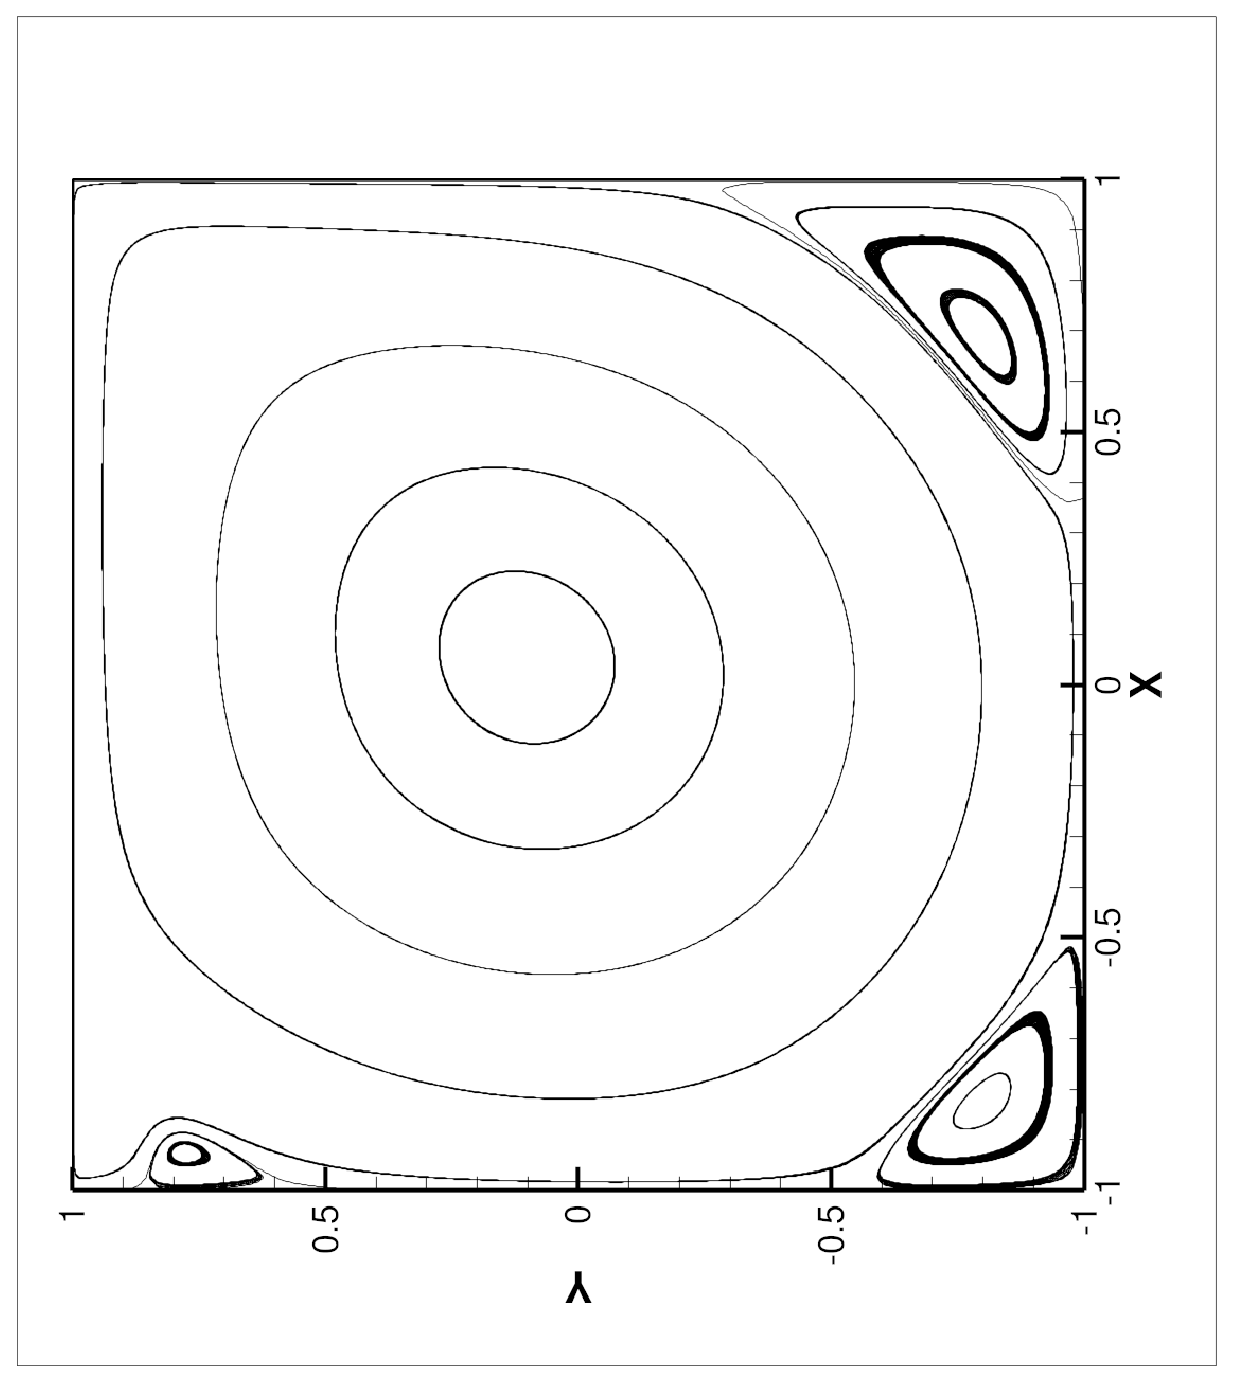
\includegraphics[width = 0.43\textwidth, angle = -90]{picture/second/second/cavity_flow_data/streamline.eps}
%        \end{center}
%        \caption{  Cavity flow: velocity streamline, pressure
%          mesh $40 \times 40$, $\nu = 0.001$.}
%        \label{fig::cavity_flow_streamline}
%       \end{figure}
%
%       \begin{figure}[!htbp]
%         \begin{center}
%             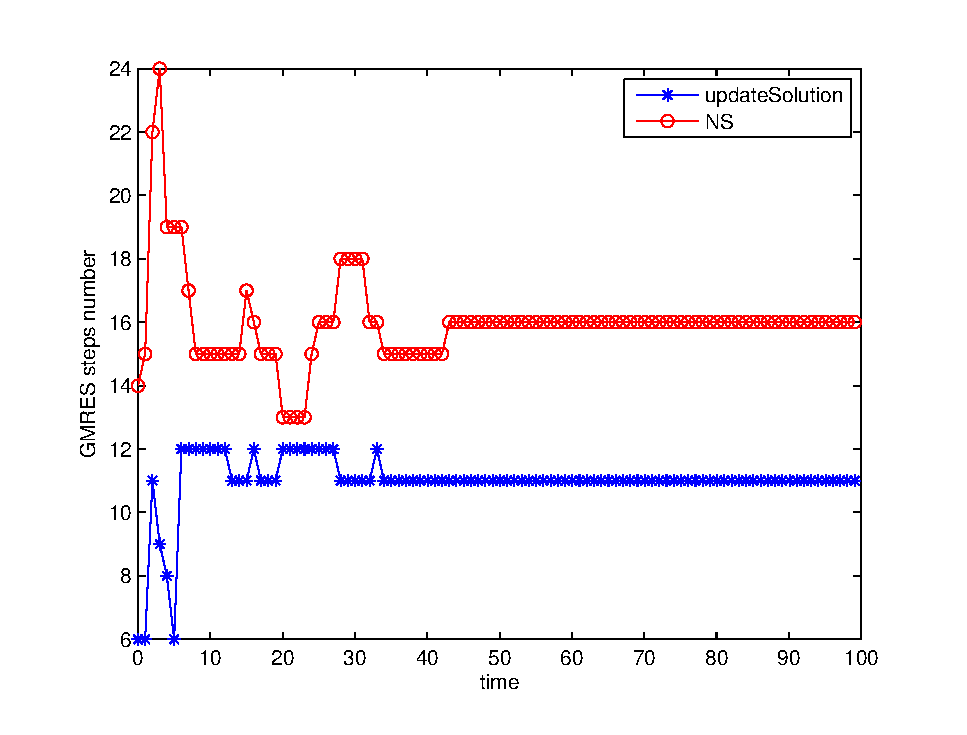
\includegraphics[width = 0.55\textwidth, angle = 0]{picture/second/second/cavity_flow_data/NS_iterate_steps.eps}
%        \end{center}
%        \caption{  Cavity flow: GMRES step counts of solving
%          ~\eqref{eq::linear_system}  with modified PCD preconditon,
%          pressure mesh $40 \times 40$, $\nu = 0.001$.}
%        \label{fig::cavity_GMRES_steps}
%       \end{figure}
%
%       \begin{table}[!htbp]
%         \centering
%         \begin{tabular}{cccc}
%           \hline
%           \multirow{2}{*}{pressure mesh}    & \multirow{2}{*}{time
%             step} & \multicolumn{2}{c}{GMRES step number} \\
%           \cline{3-4}
%            &               & $F_p = \nu A_p + W_p^n$ & $F_p = A_p + W_p^n$ \\ \hline
%           $20 \times 20$   &   $0.00656$         &      $41$           &     $8$
%           \\ \hline
%           $40 \times 40$   &   $0.00312$         &      $43$           &     $12$
%           \\ \hline
%           $80 \times 80$   &   $0.00153$   &      $48$    &     $18$
%           \\ \hline
%         \end{tabular}
%         \caption{Cavity flow: GMRES step number of solving linear system
%           (\ref{eq::linear_system}  with different $F_p$ in PCD
%           preconditioning at first time step, $\nu = 0.001$.}
%         \label{tab::GMRES_steps_initial}
%       \end{table}
   \subsection{���̨����}

      �������ģ��������徭��һ������̨�ס��ܵ��ij�����~$l = 5$���������߽�~$x = -1, y \in (0, -1)$ ���õ���~Poiseuille ������
      ~$\vec{u} = (1 - y^2, 0)^T$���ڹܵ��Ķ��˺͵׶����õ��޻��Ʊ߽�����~$\vec{u} = (0, 0)^T$����Ȼ���������ڳ����߽�~$x = 5, y \in (-1, 1)$
      �ϡ�����ѡȡճ��ϵ��Ϊ~$\nu = 0.02$����ô��~$t \rightarrow \infty$ ʱ��������������̬��


      ����ѡȡ~\eqref{eq::monitor_vorticity} Ϊ���ƺ��������ƺ����еIJ�����~$\alpha = 2.0, \beta = 2.0$������֪�������Խ��������������չ�Ĺս�
      �������������Ҫ�����������ͼ ~\ref{fig::step_flow_mesh_streamline} �У��������ڰ���ȥ�ĹսǴ���������ǵ�����һ�¡�

      Ҫ����~CFL ���������ǵļ���ʱ�䲽����~$0.008$ ���ҡ��Ա��ò�ͬ��~$M_S^*$ ��� ~\eqref{eq::full_discreted_update} ��~GMRES ����������ͼ
      ~\ref{fig::GMRES_steps_total} �и��������п��Է���ѡȡ ~$M_S^* = \frac{1}{\nu} A_p$
      �� ~$M_S^* = A_p$ ������

      \begin{figure}[!htbp]
        \centering
        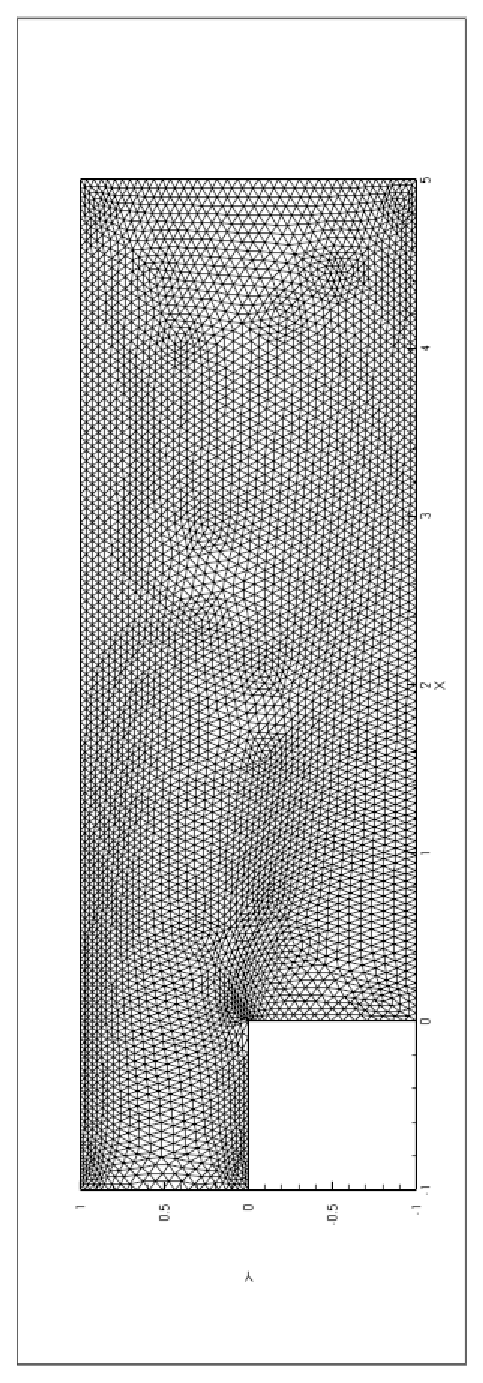
\includegraphics[width = 0.3\textwidth, angle =
        -90]{picture/second/L_shaped_flow_data/mesh.eps}
        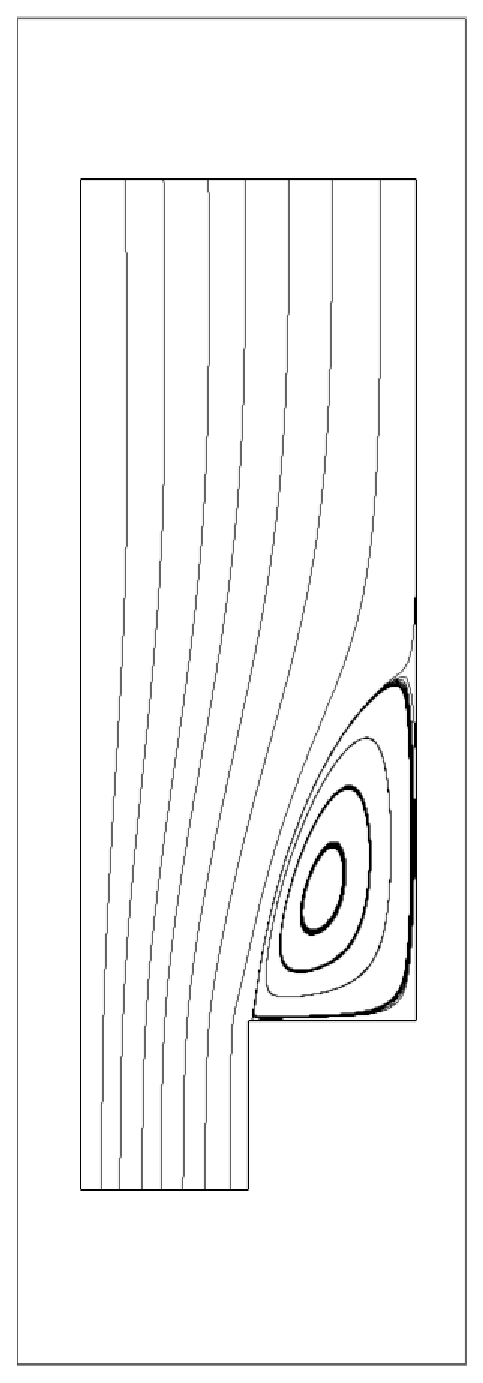
\includegraphics[width = 0.3\textwidth, angle =
        -90]{picture/second/L_shaped_flow_data/streamline.eps}
        \caption{  ���̨��������: �ƶ�������: �����ߣ�$t = 100s$��ճ��ϵ�� ~$\nu = 0.02$.}
        \label{fig::step_flow_mesh_streamline}
      \end{figure}

      \begin{figure}[!htbp]
        \centering
        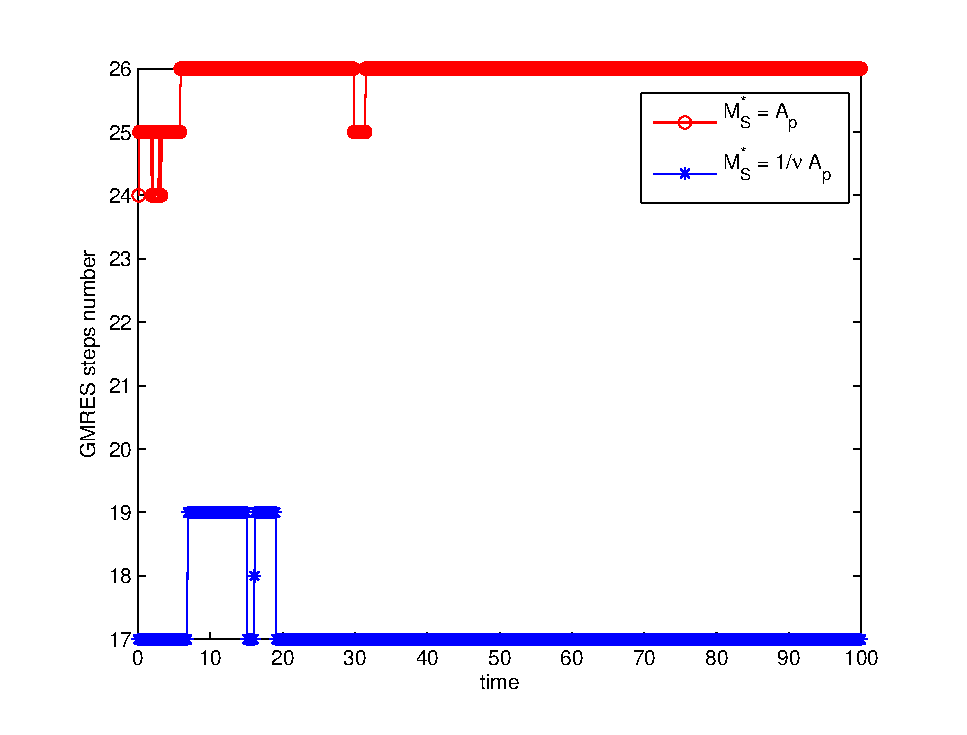
\includegraphics[width = 0.55\textwidth, angle = 0]{picture/second/L_shaped_flow_data/iteration_updateSolution.eps}
        \caption{  ���̨����: �ԱȲ�ͬ�� ~$M_S^*$ ��� ~\eqref{eq::full_discreted_update} ʱ��
        ~GMRES ��ʱ��ĵ���������$\nu = 0.02$}
        \label{fig::GMRES_steps_total}
      \end{figure}

   \subsection{Բ������}

      ��������ǵ� ~$3$ �µ�һ��������
      Բ���ϰ���Բ����~$(0, 0)$���뾶��~$r = 0.3$��
      ��ճ��ϵ�� ~$\nu = 1/300$��ͨ���򵥼�����ŵ��~$Re = \frac{2rU_{m}}{\nu} = 240$��
      ����~$U_{m}$ ������ƽ���ٶȡ����������� ~$\Omega = [-1, 5] \times [-1, 1]$���������߽�
      ~$x = -1$�����þ���~Poiseuille ���ʵı߽����� ~$\vec{u} = (1 - y^2, 0)^T$���ڹܵ����ϱ߽���±߽磬�趨����~$\vec{u} = (0, 0)^T$��
      ��Ȼ���������ڳ����߽� ~$x = 5$ �ϡ�

      �����ǵ��ƶ������У��û��������ÿ��ƺ��� ~\eqref{eq::monitor_vorticity}  �IJ���~$\alpha$ �� ~$\beta$��$\alpha$ ��ֵԽ��
      ����ۼ��ij̶Ⱦ�Խ�󡣴�ͼ ~\ref{fig::cylinder_GMRES_steps_comparation} �У����ǿ��Կ��� ~$\alpha = 5$ ʱ~GMRES �ĵ�������
      Ҫ�� ~$\alpha = 1$ ʱ�ĵ��������ࡣ�ڱ� ~\ref{tab::GMRES_steps_cylinder} �У����ǶԱ�������� ~\eqref{eq::linear_system} �� ~\eqref{eq::full_discreted_update} ʱ��Ԥ����������ѡȡ��ͬ�� ~$F_p$ �� ~$M_S^*$��GMRES ��ƽ������������
      ������֣�ѡȡ ~$F_p = \nu A + W_p^n$��GMRES ��ƽ��������������Լ��� ~$10$ �Ρ�ͬʱ��ѡȡ ~$M_S^* = \frac{1}{\nu} A_p$ �� ~$M_S^* = A_p$ �������������һ�룬���ѡȡ ~$M_S^* = \frac{1}{\nu} A_p$ ����Ч��

      ��ͼ ~\ref{fig::cylinder_mesh_2s} �У�չʾ�� ~$t = 2s$ ʱ�������ƶ�Ч�������Է��֣��������Եľۼ���Բ���ϰ������Χ����������֪��
      ��ѡȡ�ʵ�����ŵ��ʱ��������н����󣬲ο�~\cite{milton1982album} һ�ģ�����ͼ ~\ref{fig::cylinder_mesh_40s} ��չʾ�ġ�

      \begin{figure}[!htbp]
        \begin{center}
          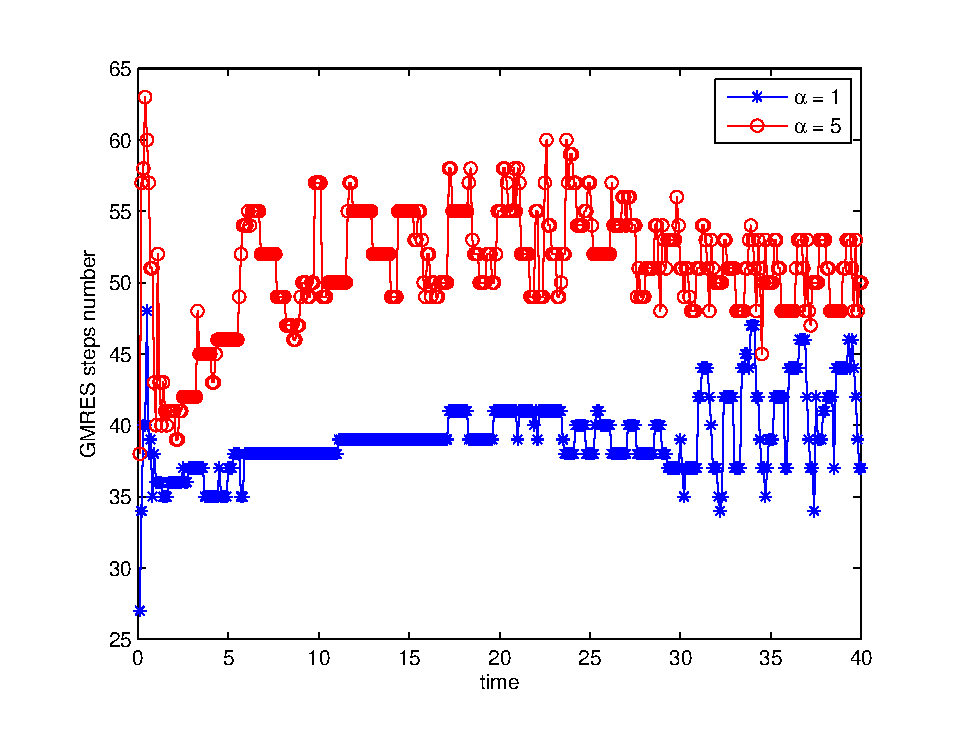
\includegraphics[width = 0.55\textwidth]{picture/second/obstacle_flow_data/iteration_steps_via_alpha.eps}
        \end{center}
        \caption{  Բ���������ԱȲ�ͬ ~$\alpha$���� ~PCD Ԥ������� ~\eqref{eq::linear_system}��GMRES �ĵ���������$Re = 240$.}
        \label{fig::cylinder_GMRES_steps_comparation}
      \end{figure}


       \begin{table}[!htbp]
         \centering
         \begin{tabular}{ccccc}
           \hline
           \multirow{3}{*}{����ϵͳ}   &  \multicolumn{4}{c}{GMRES ƽ����������} \\
           \cline{2-5}
                           & \multicolumn{2}{c}{$F_p = A + W_p^n $} &
                           \multicolumn{2}{c}{$F_p = \nu A + W_p^n $} \\ \hline
                           & $M_S^* = \frac{1}{\nu}A_p$&  $M_S^* = A_p$ & $M_S^* = \frac{1}{\nu}A_p$  &  $M_S^* = A_p$   \\ \hline
           \eqref{eq::linear_system}         & $51.06$   & $ 45.13$ &
           $ 61.06 $   & $61.08$  \\ \hline
           \eqref{eq::full_discreted_update} & $22.25$   & $40.35$  & $ 23.77 $   & $40.78$
           \\ \hline
         \end{tabular}
         \caption{Բ���������Ա��ò�ͬ��Ԥ�������� ~$F_p$ �� ~$M_S^*$ �ֱ���� ~\eqref{eq::linear_system} �� ~\eqref{eq::full_discreted_update} ʱ��GMRES ��ƽ������������$\alpha = 5, Re = 240$��}
         \label{tab::GMRES_steps_cylinder}
       \end{table}

      \begin{figure}[!htbp]
        \centering
        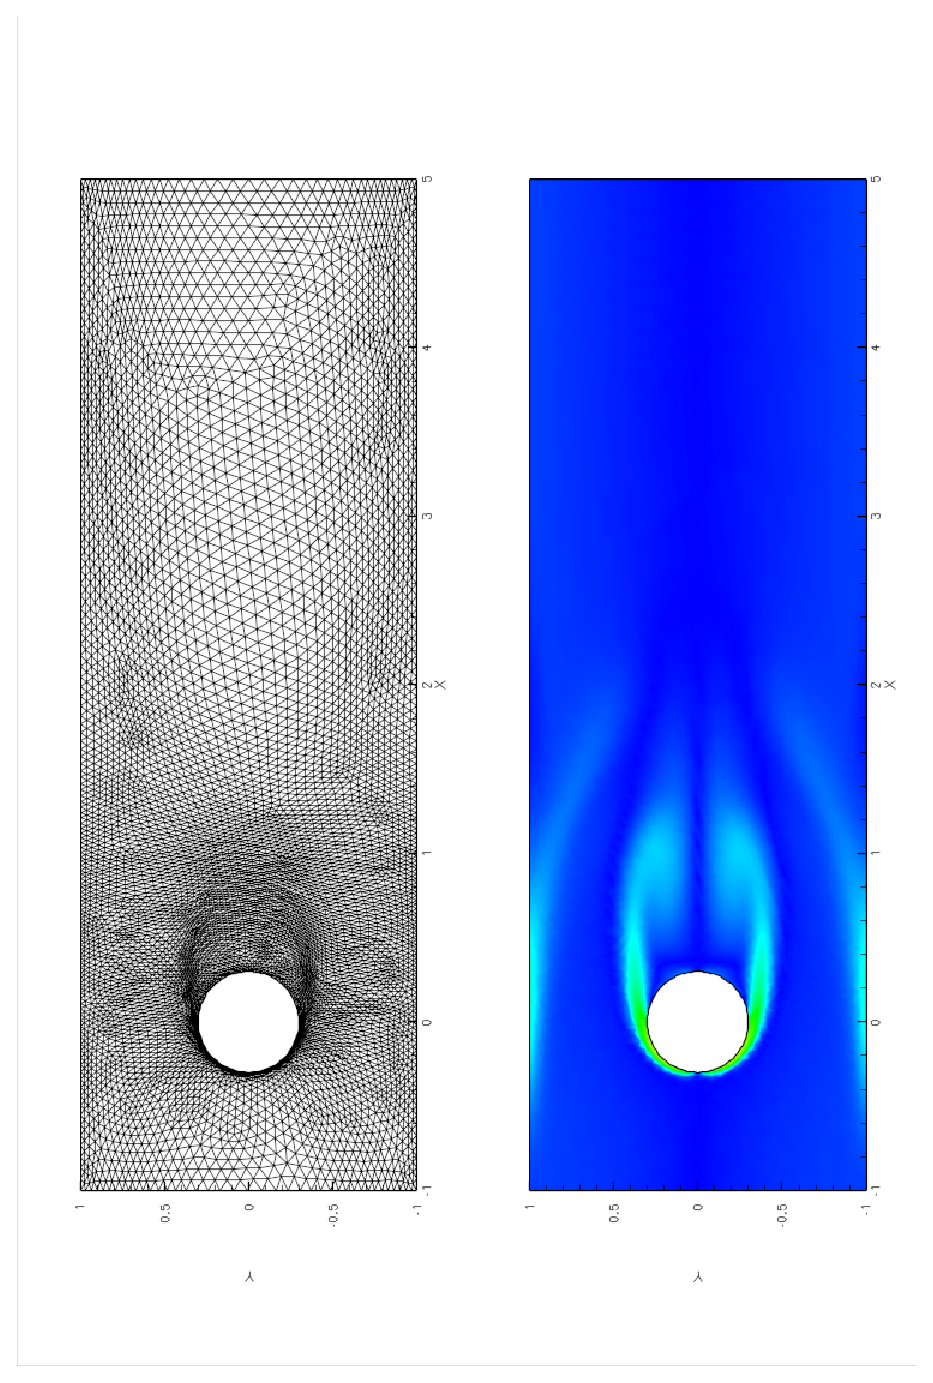
\includegraphics[width = 0.5\textwidth, angle = -90]{picture/second/obstacle_flow_data/mesh_vortex_t2s.eps}
        \caption{Բ���������ϣ��ƶ������£������ȸ��ߣ�$t = 2s$��
         $Re = 240$��}
        \label{fig::cylinder_mesh_2s}
      \end{figure}

      \begin{figure}[!htbp]
        \centering
        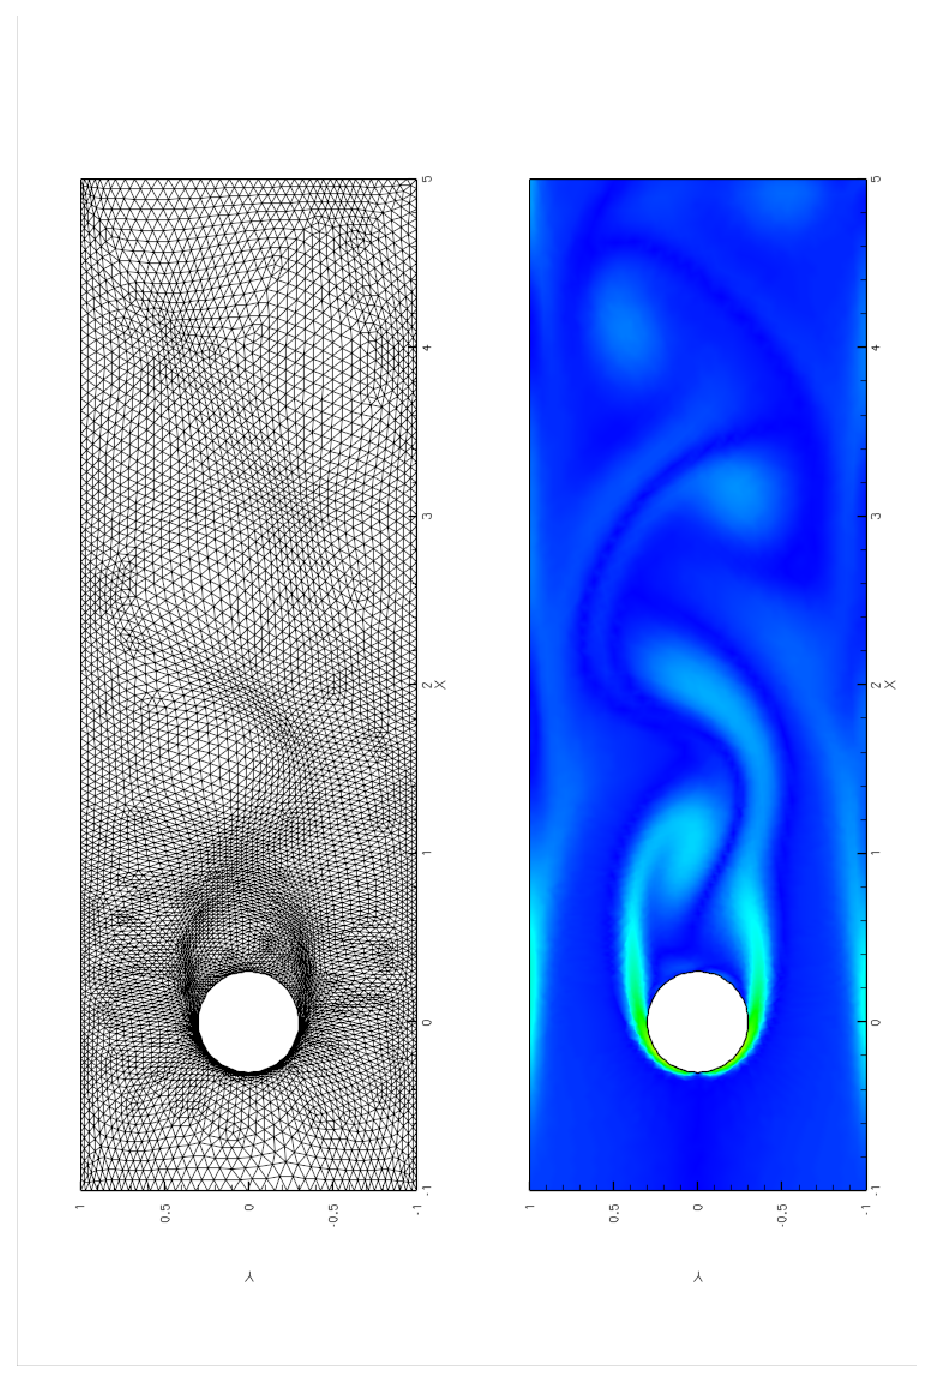
\includegraphics[width = 0.5\textwidth, angle = -90]{picture/second/obstacle_flow_data/mesh_vortex_t40s.eps}
        \caption{Բ���������ϣ��ƶ������£������ȸ��ߣ�$t = 40s$��
         $Re = 240$��}
        \label{fig::cylinder_mesh_40s}
      \end{figure}


  %=== 参考文献 ===%
  % 使用 BibTeX
  \bibliography{references/mathpaper}
  %GATHER{references/LingBib.bib}
  % 不使用BibTex
  %%%---------------------------------------------------------------------------%%
%%------------------------------ ����� -----------------------------------%%
%%---------------------------------------------------------------------------%%


\begin{thebibliography}{30}

\bibitem{Candela1990} V. Candela and A. Marquina,
Recurrence Relations for Rational Cubic Methods I: The Halley
Method, Computing, 44 (1990) 169-184.

\bibitem{Deuflhard1979} Peter Deuflhard and G. Heindl, Affine
Invariant Convergence Theorems for Newton's Method and Extensions to
Related Methods, SIAM J. Numer. Anal., 16 (1979) 1-10.

\bibitem{Deuflhard2004} Peter Deuflhard, Newton Methods for
Nonlinear Problems: Affine Invariance and Adaptive Algorithms,
Springer-Verlag, Berlin Heidelberg, 2004.

\bibitem{Deuflhard1992} Peter Deuflhard and Florian A. Potra,
Asymptotic Mesh Independence of Newton-Galerkin Methods via a
Refined Mysovskii Theorem, SIAM J. Numer. Anal., 29 (1992)
1395-1412.

\bibitem{Ezquerro2005} J.A. Ezquerro and M.A. Hern\'{a}ndez, On
the R-Order of the Hally Method, J. Math. Anal. Appl., 303 (2005)
591-601.

\bibitem{Gutierrez1997} J.M. Guti\'{e}rrez and
M.A. Hern\'{a}ndez, Third-order Iterative Methods for Operators with
Bounded Second Derivative, J. Comput. Appl. Math., 82 (1997)
171-183.

\bibitem{Gutierrez2000} J.M. Guti\'{e}rrez and
M.A. Hern\'{a}ndez, Newton's Method under Weak Kantorovich
Conditions, IMA J. Numer. Anal., 20 (2000) 521-532.

\bibitem{Kantorvich1982} L.V. Kantorvich and G.P. Akilov,
Functional Analysis, Pergamon Press, Oxford, 1982.

\bibitem{Melman1997} A. Melman, Geometry and Convergence of Euler's
and Halley's Methods, SIAM Rev., 39 (1997) 728-735.

\bibitem{Wang2000} Xinghua Wang, Convergence of Newton's Method and
Uniqueness of the Solution of Equations in Banach Space, IMA J.
Numer. Anal., 20 (2000) 123-134.

\bibitem{WangLiLai2002} Xinghua Wang, Chong Li and Mingjun Lai, A
Unified Convergence Theory for Newton-Type Methods for Zeros of
Nonlinear Operators in Banach Spances, BIT, 42 (2002) 206-213.

\bibitem{Weiser2005} Martin Weiser, Anton Schiela and Peter
Deuflhard, Asymptotic Mesh Independence of Newton's Method
Revisited, SIAM J. Numer. Anal., 42 (2005) 1830-1845.

\bibitem{XuLi2007} Xiubin Xu and Chong Li, Convergence of
Newton's Method for Systems of Equations with Constant Rank
Derivatives, J. Comput. Math., 25 (2007) 705-718.

\bibitem{XuLi2008} Xiubin Xu and Chong Li, Convergence Criterion
of Newton's Method for Singular Systems with Constant Rank
Derivatives, J. Math. Anal. Appl., 345 (2008) 689-701.

\bibitem{Yao1999} Qingchuan Yao, On Halley Iteration, Numer. Math.,
81 (1999) 647-677.

\bibitem{YeLi2006} Xintao Ye, Chong Li, Convergence of the
Family of the Deformed Euler-Hally Iterations under the H\"{o}lder
Condition of the Second Derivative, J. Comput. Appl. Math., 194
(2006) 294-308.

\end{thebibliography}



  %=== 附录 ===%
%  \appendix
%  \include{Chapters/chaptersrequires}


%%===========================================================================%%
%%========================= 附件部分 ========================================%%
%%===========================================================================%%

%它不再对章进行自动编号,但不改变页码数字格式,不重设页码计数器
\backmatter


  %=== 发表文章目录 ===%
%  %%---------------------------------------------------------------------------%%
%%----------------------------- �о��ɹ� ------------------------------------%%
%%---------------------------------------------------------------------------%%
\begin{publications}{20}

\item
An analysis on efficiency of Euler's method for computing the matrix
pth root, 2013, in preparation.

\item
A note on Newton's method and Halley's method for computing the
matrix pth root, 2013, in preparation.

\item
On the semilocal convergence behavior for Halley's method, Comput.
Optim. Appl., 2014.

\item
A globally convergent inexact Newton-like Cayley transform method
for inverse eigenvalue problems, J. Appl. Math., 2013.

\item
Convergence behavior for Newton-Steffensen's method under
gamma-condition of second derivative, Abstr. Appl. Anal., 2013.

\end{publications}


    %=== 致谢 ===%
%  %%---------------------------------------------------------------------------%%
%%------------------------------- ��л --------------------------------------%%
%%---------------------------------------------------------------------------%%




\begin{thanks}
�������ڻ�������ڣ���������ڵ�Ϥ��ָ������ɵġ�
�dz���л��λ��ʦ����ѧϰ�������ϵ�ָ���͹ػ��������Ͻ���ѧ��֪ʶԨ����ǫ�����
ʹ�������dz��Ϊ���ṩ�����õ�ѧϰ��Χ�ͻ������dz���л��λ��ʦ�����ҵĹ�����֧�֣�
�����������Գ�ߵľ���ͳ�ֿ��л�⣡

��л�㽭��ѧ��ѧ��ѧѧԺ�ĸ�λ��ʦ�������ҵĹ�����Ա����лۡ���Ƚ��ڡ���������ʿ��
����ΰ��ʿ����־�ɲ�ʿѧ���ϵ�ָ���Ͱ�������л������������������ꡢ��塢����ά��
����������ʦ��ѧϰ�ڼ�����ָ���Ͱ�������лһ��ѧϰ�����۵�������������á�
����ѩ��֣�ϡ����񷼵�ͬѧ��

����Ҹ�л�ҵļ��ˣ���л��ĸ��˽�Ĺذ���֧�֡���л���й����ҡ�֧���ҡ�������
�����˺������ǣ�
\end{thanks}


  %=== 学位论文独创性声明和学位论文使用授权声明 ===%
%  %%---------------------------------------------------------------------------%%
%%------------------------------- ���� --------------------------------------%%
%%---------------------------------------------------------------------------%%

\
\newpage

\begin{minipage}{15cm}
\begin{OriginalityStatements}
\

\setlength{\parindent}{2em}
�����������ʽ���ѧλ�������Ҹ����ڵ�ʦָ����
���е��о�������ȡ�õ��о��ɹ���
�����г����ر���Ա�ע����л�ĵط��⣬
�����������˻����������Ѿ�������׫д�����о��ɹ���
����ͬ־�Ա��о��������������Ĺ��׾�������������
����ȷ����������ʾ��л�⣮
������ȫ��ʶ���������ķ��ɽ���ɱ��˳е���
\newline
\newline

\CASTspace ����ǩ����\CASTspace \CASTspace \CASTspace \CASTspace
\CASTspace ���ڣ�\CASTspace \CASTspace �� \CASTspace �� \CASTspace
��
\\[3cm]
\end{OriginalityStatements}



\begin{LicenseStatements}
\

\setlength{\parindent}{2em}
������ȫ�˽��㽭��ѧ�йر�����ʹ��ѧλ���ĵĹ涨��
����ѧУ��Ȩ������������йػ��ػ�����ͽ����ĵĸ�ӡ���͵����ĵ���
�������ı����ĺͽ��ģ����Բ���Ӱӡ����ӡ��ɨ����ֶα��桢���ѧλ���ģ�
ͬ���㽭��ѧ�����ò�ͬ��ʽ�ڲ�ͬý���Ϸ������������ĵ�ȫ���򲿷����ݣ�

���ܵ�ѧλ�����ڽ��ܺ����ش�Э�飮
\newline
\newline

\noindent ����ǩ����\CASTspace \CASTspace \CASTspace
��ʦǩ����\CASTspace \CASTspace \CASTspace ���ڣ�\CASTspace
\CASTspace �� \CASTspace �� \CASTspace ��

\end{LicenseStatements}
\end{minipage}



\end{document}
